\documentclass[twoside,11pt]{report}
% available document structure commands :
% Report: \part{}, \chapter{}, \section{}, \subsection{}, \subsubsection{}, \paragraph{}, \subparagraph{}.

% encoding
\usepackage[utf8]{inputenc}

% maths packages
\usepackage{amsmath}
\usepackage{amssymb}
\usepackage{amsthm}
\usepackage{mathrsfs}
\usepackage{array}
\usepackage{thmtools}
\usepackage{bbm}

% mise en forme
% -------------

% base
% https://www.overleaf.com/learn/latex/Page_size_and_margins
\usepackage[a4paper]{geometry}
\newgeometry{
    top=2cm,
    bottom=2cm,
    outer=2cm,
    inner=2cm    
}
% % to have paysage
\usepackage{pdflscape}
% % paragraph management
% % https://mirror.ox.ac.uk/sites/ctan.org/macros/latex/contrib/parskip/parskip.pdf
% % spacing management
% % https://www.overleaf.com/learn/latex/Articles/How_to_change_paragraph_spacing_in_LaTeX
\usepackage{parskip}  
% % code highlighting
% % https://www.overleaf.com/learn/latex/Code_Highlighting_with_minted
\usepackage{minted}
% % draw arrows on side of aligned equations
% % https://mirrors.ibiblio.org/CTAN/macros/generic/witharrows/witharrows.pdf
\usepackage{witharrows}
% % graphiques
% % https://www.overleaf.com/learn/latex/TikZ_package
\usepackage{tikz, pgfplots}
\pgfplotsset{compat=1.18}
\usetikzlibrary{positioning, arrows.meta}
\usetikzlibrary{bayesnet}
\usetikzlibrary[quotes]
\usetikzlibrary{arrows}
\usetikzlibrary{backgrounds}
\usetikzlibrary{shapes, shapes.geometric, shapes.misc}
% % graphicx
% % https://fr.overleaf.com/learn/latex/Inserting_Images
\usepackage{graphicx}
\graphicspath{ {./images/figure} }
% % verbatim
% % https://texdoc.org/serve/fancyvrb/0
\usepackage{fancyvrb}
% % headers, footers
% % https://www.overleaf.com/learn/latex/Headers_and_footers
\usepackage{fancyhdr}
% % chapter headings
% % https://texblog.org/2012/07/03/fancy-latex-chapter-styles/
% %Options: Sonny, Lenny, Glenn, Conny, Rejne, Bjarne, Bjornstrup
\usepackage[Bjornstrup]{fncychap}
% % colors !
% % https://fr.overleaf.com/learn/latex/Using_colors_in_LaTeX
\usepackage{color}
\usepackage{xcolor}
% % color boxes
% % https://www.tug.org/docs/latex/tcolorbox/tcolorbox.pdf
\usepackage{tcolorbox}
\usepackage{xparse}
\tcbuselibrary{theorems, skins, breakable}
% %\newtheorem{theorem}{Theorem}[section]
% %\newtheorem{definition}{Definition}[section]
% % multicolmuns
\usepackage{multicol}
\setlength{\columnsep}{0.5cm}
% % package to have text in boxes
\usepackage[]{mdframed}
% % glossaries
% % https://www.overleaf.com/learn/latex/Glossaries
\usepackage{glossaries}
\makeglossaries
% % multicolomuns
\usepackage{multicol}
% % algos
\usepackage{algorithm}
\usepackage{algorithmic}
% % https://ctan.tetaneutral.net/macros/latex/contrib/titlesec/titlesec.pdf
\usepackage{titlesec}
% % appendix and reference
\usepackage[backend=biber]{biblatex}
\usepackage[toc,page]{appendix}
% % to display tables
\usepackage{booktabs}
% % https://fr.wikibooks.org/wiki/LaTeX/Tableaux
% % https://ctan.mines-albi.fr/macros/latex/contrib/arydshln/arydshln-man.pdf
\usepackage{tabularx}
\usepackage{arydshln}
% % epigraph
\usepackage{epigraph}
% % quotes
\usepackage{csquotes}
% % to test
\usepackage{lipsum}
% % for conditional independence symbol \Perp
\usepackage{txfonts}
% % nicer toc
\usepackage{tocloft}
\setlength{\cftchapindent}{2em}
% % arrows in equations
\usepackage{witharrows}
\usepackage{setspace}
% % links
% % https://fr.overleaf.com/learn/latex/Hyperlinks
\usepackage[colorlinks=true,urlcolor=blue]{hyperref}
% % don't know if useful
% \usepackage{caption}
% \usepackage{subcaption}
\newacronym{dag}{DAG}{Directed Acyclic Graph}
\newacronym{vae}{VAE}{Variational Auto Encoder}
\newacronym{vlb}{VLB}{Variational Lower Bound}
\newacronym{elbo}{ELBO}{Evidence Lower Bound}
\newacronym{dvae}{DVAE}{Dynamical Variational Auto Encoder}
\newacronym{lstm}{LSTM}{Long Short Term Memory}
\newacronym{mlp}{MLP}{Multi Layer Perceptron}
\newacronym{vrnn}{VRNN}{Variational Recurrent Neural Network}
\newacronym{gpm}{GPM}{Graphical Probabilistic Model}
\newacronym{gpvae}{GP-VAE}{Gaussian Process Variational Auto Encoder}
\newacronym{gp}{GP}{Gaussian Process}
\newacronym{sde}{SDE}{Stochastic Differential Equation}
\newacronym{it}{IT}{Information Theory}
\newacronym{apen}{ApEn}{Approximate Entropy}
\newacronym{sampen}{SampEn}{Sample Entropy}
\newacronym{rts}{RTS}{Rauch-Tung-Striebel}
% \makeglossaries
% conditional independence
\newcommand{\indep}{\perp \!\!\! \perp}
\newcommand{\notindep}{\not\!\perp\!\!\!\perp}
\newcommand{\cond}{\, \vert \,}
% real numbers
\newcommand{\R}{\mathbb{R}}
% expectation
\newcommand{\E}[1]{\mathbb{E}_{#1}}
% KL
\newcommand{\KL}[2]{\mathbb{KL}\left( #1 \vert\vert #2 \right)}
% VLB/ELBO
\newcommand{\VLB}{\mathcal{L}(\theta, \phi, X)}
% neural net Gaussian with diagonal covariance
\newcommand{\NNdiag}[3]{\mathcal{N}( #1 \vert #2, \text{diag}\, #3)}
% Brownian motion and related commands
\newcommand{\brownian}{(\Omega, \mathcal{F}, (\mathcal{F}_t)_{t \geq 0}, (B_t)_{t \geq 0}, \mathbb{P})}
\newcommand{\filtration}{(\mathcal{F}_t)_{t \in T}}
\newcommand{\espaceprob}{(\Omega, \mathcal{F}, \mathbb{P})}
\newcommand{\lunomega}{L^1(\Omega, \mathcal{F}, \mathbb{P})}
\newcommand{\ldeuxomega}{L^2(\Omega, \mathcal{F}, \mathbb{P})}
\newcommand{\norm}[1]{\vert \vert #1 \vert \vert}
% Theorem System
% The following boxes are provided:
%   Definition:     \defn 
%   Theorem:        \thm 
%   Lemma:          \lem
%   Corollary:      \cor
%   Proposition:    \prop   
%   Claim:          \clm
%   Fact:           \fact
%   Proof:          \pf
%   Example:        \ex
%   Remark:         \rmk (sentence), \rmkb (block)
% Suffix
%   r:              Allow Theorem/Definition to be referenced, e.g. thmr
%   p:              Add a short proof block for Lemma, Corollary, Proposition or Claim, e.g. lemp
%                   For theorems, use \pf for proof blocks

% ======= Real examples : 

% \defn{Definition Name}{
%     A defintion.
% }

% \thmr{Theorem Name}{mybigthm}{
%     A theorem.
% }

% \lem{Lemma Name}{
%     A lemma.
% }

% \fact{
%     A fact.
% }

% \cor{
%     A corollary.
% }

% \prop{
%     A proposition.
% }

% \clmp{}{
%     A claim.
% }{
%     A reference to Theorem~\ref{thm:mybigthm}
% }

% \pf{
%    proof.

% \ex{
%     some examples. 
% }

% \rmk{
%     Some remark.
% }

% \rmkb{
%     Some more remark.
% }

\usepackage{xcolor}

% Define custom colors
\definecolor{defscol}{HTML}{ecd8d7} %For definitions
\definecolor{asumscol}{HTML}{ecd8d7} %For Assumptions

\definecolor{rmkscol}{HTML}{313160} %For remarks
\definecolor{exmscol}{HTML}{e04b52} %For examples

\definecolor{lemscol}{HTML}{2c3943} %For Lemmes
\definecolor{thmscol}{HTML}{595765} %For Theorems
\definecolor{prpscol}{HTML}{9c98b1} %For proposition
\definecolor{corscol}{HTML}{dfd9fd} %For corrolaries

\definecolor{clmscol}{HTML}{165c58} %For claims
\definecolor{facscol}{HTML}{28a8a1} %For facts



% ============================
% Definition
% ============================
\newtcbtheorem[number within=section]{mydefinition}{Definition}
{
    enhanced,
    frame hidden,
    titlerule=0mm,
    toptitle=1mm,
    bottomtitle=1mm,
    fonttitle=\bfseries\large,
    coltitle=black,
    colbacktitle=defscol!40!white,
    colback=defscol!20!white,
}{defn}

\NewDocumentCommand{\defn}{m+m}{
    \begin{mydefinition}{#1}{}
        #2
    \end{mydefinition}
}

\NewDocumentCommand{\defnr}{mm+m}{
    \begin{mydefinition}{#1}{#2}
        #3
    \end{mydefinition}
}

% ============================
% Assumption
% ============================
\newtcbtheorem[use counter from=mydefinition]{myassumption}{Assumption}
{
    enhanced,
    frame hidden,
    titlerule=0mm,
    toptitle=1mm,
    bottomtitle=1mm,
    fonttitle=\bfseries\large,
    coltitle=black,
    colbacktitle=asumscol!40!white,
    colback=asumscol!20!white,
}{asum}

\NewDocumentCommand{\asum}{m+m}{
    \begin{myassumption}{#1}{}
        #2
    \end{myassumption}
}

\NewDocumentCommand{\asumr}{mm+m}{
    \begin{myassumption}{#1}{#2}
        #3
    \end{myassumption}
}

% ============================
% Theorem
% ============================

\newtcbtheorem[use counter from=mydefinition]{mytheorem}{Theorem}
{
    enhanced,
    frame hidden,
    titlerule=0mm,
    toptitle=1mm,
    bottomtitle=1mm,
    fonttitle=\bfseries\large,
    coltitle=black,
    colbacktitle=thmscol!40!white,
    colback=thmscol!20!white,
}{thm}

\NewDocumentCommand{\thm}{m+m}{
    \begin{mytheorem}{#1}{}
        #2
    \end{mytheorem}
}

\NewDocumentCommand{\thmr}{mm+m}{
    \begin{mytheorem}{#1}{#2}
        #3
    \end{mytheorem}
}

\newenvironment{thmpf}{
	{\noindent{\it \textbf{Proof for Theorem.}}}
	\tcolorbox[blanker,breakable,left=5mm,parbox=false,
    before upper={\parindent15pt},
    after skip=10pt,
	borderline west={1mm}{0pt}{thmscol!40!white}]
}{
    \textcolor{thmscol!40!white}{\hbox{}\nobreak\hfill$\blacksquare$} 
    \endtcolorbox
}

\NewDocumentCommand{\thmp}{m+m+m}{
    \begin{mytheorem}{#1}{}
        #2
    \end{mytheorem}

    \begin{thmpf}
        #3
    \end{thmpf}
}

% ============================
% Lemma
% ============================

\newtcbtheorem[use counter from=mydefinition]{mylemma}{Lemma}
{
    enhanced,
    frame hidden,
    titlerule=0mm,
    toptitle=1mm,
    bottomtitle=1mm,
    fonttitle=\bfseries\large,
    coltitle=black,
    colbacktitle=lemscol!40!white,
    colback=lemscol!20!white,
}{lem}

\NewDocumentCommand{\lem}{m+m}{
    \begin{mylemma}{#1}{}
        #2
    \end{mylemma}
}

\newenvironment{lempf}{
	{\noindent{\it \textbf{Proof for Lemma}}}
	\tcolorbox[blanker,breakable,left=5mm,parbox=false,
    before upper={\parindent15pt},
    after skip=10pt,
	borderline west={1mm}{0pt}{lemscol!40!white}]
}{
    \textcolor{lemscol!40!white}{\hbox{}\nobreak\hfill$\blacksquare$} 
    \endtcolorbox
}

\NewDocumentCommand{\lemp}{m+m+m}{
    \begin{mylemma}{#1}{}
        #2
    \end{mylemma}

    \begin{lempf}
        #3
    \end{lempf}
}

% ============================
% Corollary
% ============================

\newtcbtheorem[use counter from=mydefinition]{mycorollary}{Corollary}
{
    enhanced,
    frame hidden,
    titlerule=0mm,
    toptitle=1mm,
    bottomtitle=1mm,
    fonttitle=\bfseries\large,
    coltitle=black,
    colbacktitle=corscol!40!white,
    colback=corscol!20!white,
}{cor}

\NewDocumentCommand{\cor}{+m}{
    \begin{mycorollary}{}{}
        #1
    \end{mycorollary}
}

\newenvironment{corpf}{
	{\noindent{\it \textbf{Proof for Corollary.}}}
	\tcolorbox[blanker,breakable,left=5mm,parbox=false,
    before upper={\parindent15pt},
    after skip=10pt,
	borderline west={1mm}{0pt}{corscol!40!white}]
}{
    \textcolor{corscol!40!white}{\hbox{}\nobreak\hfill$\blacksquare$} 
    \endtcolorbox
}

\NewDocumentCommand{\corp}{m+m+m}{
    \begin{mycorollary}{}{}
        #1
    \end{mycorollary}

    \begin{corpf}
        #2
    \end{corpf}
}

% ============================
% Proposition
% ============================

\newtcbtheorem[use counter from=mydefinition]{myproposition}{Proposition}
{
    enhanced,
    frame hidden,
    titlerule=0mm,
    toptitle=1mm,
    bottomtitle=1mm,
    fonttitle=\bfseries\large,
    coltitle=black,
    colbacktitle=prpscol!30!white,
    colback=prpscol!20!white,
}{prop}

\NewDocumentCommand{\prop}{+m}{
    \begin{myproposition}{}{}
        #1
    \end{myproposition}
}

\newenvironment{proppf}{
	{\noindent{\it \textbf{Proof for Proposition.}}}
	\tcolorbox[blanker,breakable,left=5mm,parbox=false,
    before upper={\parindent15pt},
    after skip=10pt,
	borderline west={1mm}{0pt}{prpscol!40!white}]
}{
    \textcolor{prpscol!40!white}{\hbox{}\nobreak\hfill$\blacksquare$} 
    \endtcolorbox
}



\NewDocumentCommand{\propp}{+m+m}{
    \begin{myproposition}{}{}
        #1
    \end{myproposition}

    \begin{proppf}
        #2
    \end{proppf}
}

% ============================
% Claim
% ============================

\newtcbtheorem[use counter from=mydefinition]{myclaim}{Claim}
{
    enhanced,
    frame hidden,
    titlerule=0mm,
    toptitle=1mm,
    bottomtitle=1mm,
    fonttitle=\bfseries\large,
    coltitle=black,
    colbacktitle=clmscol!40!white,
    colback=clmscol!20!white,
}{clm}

\NewDocumentCommand{\clm}{m+m}{
    \begin{myclaim*}{#1}{}
        #2
    \end{myclaim*}
}

\newenvironment{clmpf}{
	{\noindent{\it \textbf{Proof for Claim.}}}
	\tcolorbox[blanker,breakable,left=5mm,parbox=false,
    before upper={\parindent15pt},
    after skip=10pt,
	borderline west={1mm}{0pt}{clmscol!40!white}]
}{
    \textcolor{clmscol!40!white}{\hbox{}\nobreak\hfill$\blacksquare$} 
    \endtcolorbox
}

\NewDocumentCommand{\clmp}{m+m+m}{
    \begin{myclaim*}{#1}{}
        #2
    \end{myclaim*}

    \begin{clmpf}
        #3
    \end{clmpf}
}

% ============================
% Fact
% ============================

\newtcbtheorem[use counter from=mydefinition]{myfact}{Fact}
{
    enhanced,
    frame hidden,
    titlerule=0mm,
    toptitle=1mm,
    bottomtitle=1mm,
    fonttitle=\bfseries\large,
    coltitle=black,
    colbacktitle=facscol!40!white,
    colback=facscol!20!white,
}{fact}

\NewDocumentCommand{\fact}{+m}{
    \begin{myfact}{}{}
        #1
    \end{myfact}
}

% ============================
% Proof
% ============================

\NewDocumentCommand{\pf}{+m}{
    \begin{proof}
        [\noindent\textbf{Proof.}]
        #1
    \end{proof}
}

% ============================
% Example
% ============================


\newenvironment{myexample}{
    \tcolorbox[blanker,breakable,left=5mm,parbox=false,
    before upper={\parindent15pt},
    after skip=10pt,
	borderline west={1mm}{0pt}{clmscol!40!white}]
}{
    \textcolor{clmscol!40!white}{\hbox{}\nobreak\hfill$\blacksquare$} 
    \endtcolorbox
}

\NewDocumentCommand{\exm}{m+m}{
    \begin{myexample}
	{\noindent{\it \textbf{Example : #1 }}}\\ 
        #2
    \end{myexample}
}


% ============================
% Remark
% ============================


\NewDocumentCommand{\rmk}{+m}{
    {\it \color{rmkscol!40!white}#1}
}

\newenvironment{remark}{
    \par
    \vspace{5pt}
    \begin{minipage}{\textwidth}
        {\par\noindent{\textbf{Remark.}}}
        \tcolorbox[blanker,breakable,left=5mm,
        before skip=10pt,after skip=10pt,
        borderline west={1mm}{0pt}{rmkscol!20!white}]
}{
        \endtcolorbox
    \end{minipage}
    \vspace{5pt}
}

\NewDocumentCommand{\rmkb}{+m}{
    \begin{remark}
        #1
    \end{remark}
}













% % Old styles hh 

% %--------------------------------------------------------------------------
% % 		THEOREMES STYLE
% %--------------------------------------------------------------------------

% %-------		DEFINITION 		-------	
% \newcounter{defo}[chapter]
% \newenvironment{defi}[1]{\refstepcounter{defo} 
% \begin{tcolorbox}[colback=yellow!20!white,colframe=yellow!15!black,title= \textbf{Définition \thechapter \ $\blacklozenge$ \thedefo \ | #1}]}{\end{tcolorbox}}

% %-------		THEOREME 		-------	
% \newcounter{th}[chapter]
% \newenvironment{thm}[1]{\refstepcounter{th}
% \begin{tcolorbox}[colback=mycolor!10,colframe=mycolor!10!black!80,title=\textbf{ Théorème \thechapter \ $\blacklozenge$ \theth \ | #1}]}{\end{tcolorbox}}

% %-------		PROPOSITION 		-------	
% \newcounter{prop}[chapter]
% \newenvironment{propt}[1]{\refstepcounter{prop}
% \begin{tcolorbox}[colback=mycolor!5,colframe=mycolor!10!linkscolor!80 ,title=\textbf{ Proposition \thechapter \ $\blacklozenge$ \theprop \ | #1}]}{\end{tcolorbox}}

% %-------		COROLLAIRE		-------
% \newcounter{cor}[chapter]
% \newenvironment{corr}[1]{\refstepcounter{cor}
% \begin{tcolorbox}[colback=mycolor!2,colframe=mycolor!10!linkscolor!40 ,title= Corolaire \thechapter \ $\blacklozenge$ \thecor \ | #1]}{\end{tcolorbox}}

% %-------		LEMME			-------
% \newcounter{lem}[chapter]
% \newenvironment{lemme}[1]{\refstepcounter{lem}
% \begin{tcolorbox}[colback=mycolor!10!blue!2,colframe=mycolor!50!blue!30,title=\textbf{Lemme \thechapter \ $\blacklozenge$ \thelem \ | #1}]}{\end{tcolorbox}}

% %-------		METHODE 			-------
% \newcounter{met}[chapter]
% \newenvironment{meth}[1]{\refstepcounter{met}
% \begin{tcolorbox}
% [enhanced jigsaw,breakable,pad at break*=1mm,
%  colback=red!20!white,boxrule=0pt,frame hidden,
%  borderline west={1.5mm}{-2mm}{red}] \color{red}
% {\textbf{Méthode \thechapter \ $\blacklozenge$ \themet \ | #1} } \color{black} \\ } {\end{tcolorbox}}

% %-------		REMARQUE 			-------
% \newcommand{\NB}[1]{
% \ \\
% \begin{tabular}{p{0.05\textwidth}p{0.80\textwidth}}
% \hline
% \vspace{-0.1cm} \includegraphics[scale=0.03]{./system/IDEA.png} & 	#1\\
% \hline
% \end{tabular}
% \ 
% \newline \ \newline
%  }

% %-------		EXEMPLE  		-------
% \newenvironment{exm}{ \begin{tcolorbox}
% [enhanced jigsaw,breakable,pad at break*=1mm,
%  colback=cyan!20!white,boxrule=0pt,frame hidden,
%  borderline west={1.5mm}{-2mm}{cyan}] \color{cyan}
% {\textbf{Exemple} } \color{black} \\ } {\end{tcolorbox}}
 


% files for bibliography
% \addbibresource{chapter/references.bib}
\addbibresource{chapter/citations.bib}
% \addbibresource{chapters/citations_2.bib}


\title{Dynamical Variational Autoencoders :\\ discrete-time and continuous-time models.\\ Links to stochastic calculus and stochastic differential equations\\
\vspace{2cm}
{\Large{ENS Paris-Saclay, MVA}}}

\author{
Benjamin Deporte\\
\href{mailto:benjamin.deporte@ens-paris-saclay.fr}{benjamin.deporte@ens-paris-saclay.fr}\\
\href{mailto:benjamin.deporte@polytechnique.org}{benjamin.deporte@polytechnique.org}% student 1
}

\date{September 2025}

\begin{document}

\everymath{\displaystyle}
\maketitle

\chapter{Remerciements}\label{sec:Remerciements}

Avec ce travail sur les VAEs dynamiques se tourne une page siginificative de mon parcours en machine learning.

Un grand merci à Pierre-Alexandre Mattei de l'INRIA, qui a accepté d'etre mon enseignant référent pour cette aventure !
Toujours disponible, bienveillant et patient devant les pires de mes questions, avec des idées et l'expérience 
pour me débloquer aux moments clefs ! Merci également à Pierre Latouche, avec lequel Pierre-Alexandre a assuré 
le cours "Introduction to Probabilistic Graphical Models and Deep Generative Models" au 1er trimestre du MVA.

Merci également à l'équipe du MVA : direction, enseignants, administration. Le Master marche bien, j'y ai appris 
énormément de nouvelles choses et consolidé des connaissances plus anciennes. L'enseignement y est bienveillant sans 
etre laxiste, exigeant et productif. Une belle formation, et à titre personnel une belle aventure Francilienne 
pendant quelques mois ! Note à Laurent Oudre : je parle un peu de séries temporelles dans ce rapport, pas mal de 
calcul stochastique, mais pas un mot sur les maths financières, promis !

A mes collègues de l'IRT : merci Lionel ! Me permettre de cumuler mon poste et le MVA pendant une petite année a 
représenté beaucoup pour moi. Toutes les organisations et tous les managers ne l'auraient pas permis, loin de là. 
Aux collègues du 6e étage du B612 - Greg, Franck, Lucas, Sebastien... : oui ma densité de probabilité a chuté, 
mais elle s'apprete à remonter ! Ne revendez pas tout de suite le mobilier de bureau. A bientot.

A mon épouse Anne-Laure, si jamais elle lit ce rapport pour s'endormir : j'étais sincère quand je disais tenter le MVA en deux ans 
parce que ce serait le plus raisonnable en terme d'emploi du temps. Mais la logique Bayesienne, après tout, est de changer d'avis 
en fonction des données disponibles. Et avouons-le, je n'ai jamais été du genre patient. Merci à toi.

A Jean-Michel Loubes - qui m'a mis le pied à l'étrier il y a quelques temps déjà, pointé vers les bons textes de référence, fait 
rencontrer beaucoup de monde pour valider ce qui, à l'époque, n'était qu'une piste d'évolution professionnelle parmis d'autres. 
Revenir aux maths, et venir au machine learning, aura été un de mes meilleurs moves professionnels. J'ai retrouvé une envie 
intellectuelle que je n'avais plus connue depuis longtemps : merci à toi. 
Merci également de m'avoir accepté en MAPI3 à Paul Sabatier il y a de cela quelque temps maintenant.

J'oublie probablement du monde, et je m'en excuse par avance. Merci en tout cas de m'avoir accompagné.

Place aux VAEs dynamiques.

\newpage
\singlespacing
\tableofcontents

\newpage
\listoffigures

\part{Introduction}
    
    % \chapter{Subject}\label{sec:Subject}

% * means no number
% \chapter*{Abstract}

\glspl{vae} are a well-known class of generative models, described in \cite{kingma_introduction_2019}, and have spawn numerous applications. However, the original i.i.d. 
assumption over the latent variables carry strong limitations when considering data sequences over time. 
A richer class of models aims at solving this limitation : the \glspl{dvae}. In \glspl{dvae}, the latent variables are structured themselves as a correlated set (usually a sequence also),
 aiming at encoding the temporal dimension of the data. 

The first part of the report is dedicated to the general study of \glspl{dvae}. A great survey is \cite{girin_dynamical_2022} and is the basis for this part. 
We review the general formulation of \glspl{dvae} and then review the detailed implementation of two discrete time models : the Deep Kalman filter, and the \gls{vrnn}. 
If a discrete-time setting of the latent variables is straightforward -for example, structuring the latent variables as a first-order Markov chain-, this setting carries limitations too. 
The first, and possibly most important one, is that the structure of the model requires regularly-sampled data. In practice, data measurements can be made 
with a changing frequency. A natural idea is then to structure the latent variables as a continuous-time process, which allows irregularly sampled data. 
A natural continuous-time process, with "nice" properties, is the \gls{gp} \cite{rasmussen_gaussian_2008} : this is the \gls{gpvae} model, that we review.
This idea is mentionned briefly in \cite{girin_dynamical_2022}, and described in more details in \cite{casale_gaussian_2018}, 
\cite{fortuin_gp-vae:_2020}, \cite{titsias_bayesian_2010} and \cite{zhu_markovian_2023}. 

The second part review the implementations of those three models, the experiments run on toy datasets, and some take-aways.
The code is available at \href{https://github.com/BenjaminDeporte/MVA_Stage}{GitHub repo}.

The paper \cite{zhu_markovian_2023} has triggered in me a significant interest. It links \gls{gpvae} with \glspl{sde}, and specifically linear \glspl{sde}. 
The linear \gls{sde} formulation of the \gls{gp} regression problem allows a computation that scales linearly using off the shelf filtering and smoothing algorithms,
rather than "naive" cubic \gls{gp} regression algorithms. 

I invested a significant amount of time in studying the mathematical machinery required to fully understand the underlying hypothesis. 
The theory of stochastic calculus is fascinating, demanding, and fruitful.
Among good study books, are \cite{mouvement-brownien-calcul-ito} and \cite{sarkka_applied_2019}. 
Getting up to speed on stochastic calculus has been quite a challenge given the time frame but proved extremely useful. 
In the following part, we present some key results, which the knowledgeable reader on stochastic calculus can skip, 
and added a longer reference at the end of this report. 

We then describe the link between the \gls{dvae} and the \gls{sde}. The solution of a general \gls{sde} is a Markov process 
in which the evolution over time of the transition probability density is described by the Fokker-Plank-Kolmogorov equation. 
Integrating that equation between two time stamps, produces a natural framework our first two discrete models : deep Kalman filter and \gls{vrnn}.
(Another well known  use-case is diffusion models). 

In the case of a linear \gls{sde}, the solution is also a Gaussian process, which links to \gls{gpvae}. 
This also allows to use off the shelf smoothers (and filters), such as Kalman and \gls{rts}, that scale linearly.
However, the \gls{gpvae} model carries limitations too. First, some Gaussian processes -more specifically some kernel functions- can not be formulated as the solution to a linear \gls{sde}.
Second, if there is an intersection between Markov processes and Gaussian processes (for example the well-studied Ornstein Uhlenbeck process), some Markov processes 
(ie solutions to general \gls{sde}) are not Gaussian processes.

An idea is then to use more general stochastic processes, derived from general (ie non-linear) \gls{sde}, that are still 
Markov processes and allow filtering. Using general \gls{sde} is a recent research field, drawing upon the theory of \gls{ode}.
We present in the complements an overview of \gls{neural-ode} and \gls{neural-sde}.

Last, along with this study, we also provide an overview of the information theory framework for data sequences -specifically some results on entropy rates-
 to empirically  quantify the degree of "randomness" (of, more accurately, uncertainty) of data sequences.
    % \chapter{Report Outline}\label{sec:outline}

\textbf{Part II} covers the mathematical background that is required for most of the report. Section 1 covers the main results regarding stochastic processes and introduces the Brownian motion. (Stochastic Differential Equations are introduced later in Part III). Section 2 recaps the main first definitions and results regarding information theory, its application to stochastic processes, some theoretical results for stationary processes and experimental metrics.

\textbf{Part II} covers discrete-time dynamical Variational AutoEncoders. Section 1 is a recap of graphical models and D-Separation, that is used throughout the report. Section 2 introduces the generic formulation of DVAEs : generative and inference models, variational lower bound. Section 3 presents the first, and most simple model : the Deep Kalman Filter. Section 4 presents the most expressive model, ie the Variationnal RNN. Section 5 is a summary of the take-aways regarding the PyTorch-implementations.

\textbf{Part III} takes us to continuous-time Dynamical VAEs. Section 1 is a recap of the theory regarding Gaussian Processes, that will be at the core of this part. Section 2 is intended to be a self-sustained presentation of the stochastic calculus, where we go quickly over the construction of the Ito's integral to derive the necessary Ito's lemma and subsequent calculation rules for the rest of the report.  Section 3 presents the GP-VAE model. Section 4 is a summary of the take-aways regarding the PyTorch implementation.

\textbf{Part IV} summarizes the experiments : Blembet UK tides, Brownian motion, O.U + Student observation model, cryptos...

\textbf{Part V} is an opening to what could be covered next ! Section 1 presents the link between SDEs and Markovian kernel Gaussian Processes. Section 2 presents some results regarding information theory and stochastic processes.
    % \chapter{Related work}\label{sec:related_work}

\lipsum[1-2]

%
%
%---------------------- DYNAMICAL VAE ---------------------------------------------
%
%
\part{Dynamical Variational Autoencoders - Theory}

This part presents the general framework of \glspl{dvae}, based on \cite{girin_dynamical_2022}. 

We start with a reminder of the key notion of \textbf{D-separation}, which is central in deriving conditional probabilities of \glspl{dvae} from their 
associated \glspl{gpm}.

Then, we describe three models in details:

\begin{itemize}
    \item \textbf{Deep Kalman Filter} : this model arises as the first evolution of the well-known Kalman Filter, with richer, \glspl{mlp} networks for the encoder and decoder.
    \item \textbf{Variational Recurrent Neural Network} : at the other end of the spectrum, \glspl{vrnn} provide the most expressive discrete-time formulation of the encoder and decoder.
We describe here a different implementation from the one described in \cite{girin_dynamical_2022}.
    \item \textbf{Gaussian Process Variational Auto Encoder} : in this model, the prior over the latent variables is no longer discrete, but is a \gls{gp}.
This allows for sampling data at irregular intervals. Another benefit is the use of richer kernel families to encode prior knowledge.
\end{itemize}

    \chapter{D-separation}\label{sec:D-Separation}

% \section{Graphical Models, Directed Acyclic Graph and factorization of joint probability distributions}
Graphical models are an efficient way to describe families of factorized joint distributions of a data set $(x_i)_{i=1,...,n}$ into a \gls{dag}. 

Given such a dataset, we can build a \gls{dag} where each node is indexed by an integer that is higher than the indexes of its \textit{parent} nodes, such that the joint distribution over the dataset factorizes as:

\begin{align}
p(x_1,x_2,...,x_n) = \prod_{i=1}^n p(x_i \vert pa_i)
\end{align}
where $pa_i$ is the set of parent nodes of $x_i$.\\
For example, the following \gls{dag}

% % --- ORIGINAL : WORKS ----------------------
% \begin{center}
% \begin{tikzpicture}[
%     X/.style={circle, draw=black!80, thin, minimum size=5mm}
% ]
% % nodes
% \node[X] (X1) {$x_1$};
% \node[X] (X2) [right= of X1]{$x_2$} edge [<-, thin] (X1); 
% \node[X] (X3) [below= of X1]{$x_3$} edge [<-, thin] (X1);
% \node[X] (X4) [right= of X3]{$x_4$} edge [<-, thin] (X3)
%                                     edge [<-, thin] (X1);
% \node[X] (X5) [right= of X4]{$x_5$} edge [<-, thin] (X4)
%                                     edge [<-, thin] (X2);
% \end{tikzpicture}
% \end{center}
% describes:
% \begin{align}
%     p(x_1,x_2,x_3,x_4,x_5) &= p(x_1)p(x_2\vert x_1)p(x_3\vert x_1)p(x_4 \vert x_1, x_3)p(x_5 \vert x_2, x_4)
% \end{align}

\begin{center}
\begin{tikzpicture}[
    X/.style={circle, draw=black!80, thin, minimum size=5mm}
]
% use \matrix to position the nodes
\matrix[row sep=0.25cm, column sep=1cm] {
    % first row
    \node[X] (X1) {$x_1$}; & \node[X] (X2) {$x_2$}; & \\
    & & \node[X] (X5) {$x_5$}; \\
    \node[X] (X3) {$x_3$}; & \node[X] (X4) {$x_4$}; & \\
};
% use \path to draw the edges
\path   (X1) edge[->, thin] (X2)
        (X1) edge[->, thin] (X3)
        (X1) edge[->, thin] (X4)
        (X2) edge[->, thin] (X5)
        (X3) edge[->, thin] (X4)
        (X4) edge[->, thin] (X5);
\end{tikzpicture}
\end{center}
describes:
\begin{align}
    p(x_1,x_2,x_3,x_4,x_5) &= p(x_1)p(x_2\vert x_1)p(x_3\vert x_1)p(x_4 \vert x_1, x_3)p(x_5 \vert x_2, x_4)
\end{align}

% \section{D-separation and conditional independence}

Describing a factorized joint probability distribution by a \gls{dag} allows to determine graphically whether two sets of nodes (ie random variables) are independent, conditioned on a third set of nodes. This allows subsequently to simplify the expressions of the observation models (ie $p(x \vert z)$, and/or the posterior models ($q(z \vert x)$).

\textbf{D-Separation} is the set of rules that determine whether there is conditional independence between two sets given a third one. D-Separation is well described in key books such as \cite{PRML}, \cite{ProbabilisticGraphicalModels} or \cite{ProbabilisticMachineLearning}. We will enunciate here the key concepts, and refer the interested reader to those books.

% \subsection{3-node DAG}

D-Separation is a way to find out graphically conditional (in)dependence relationships between random variables, that would be more difficult to calculate by marginalizing the joint distribution over the conditioning variables. A nice way to demonstrate this, is to review the three examples of 3-node \gls{dag}. 
NB : The observed (ie conditioning) variables are noted with gray background.

% --- EXAMPLE 1 ---------------------------------
\setlength{\columnsep}{1.5cm}
\begin{multicols}{3}[
\textbf{Example 1} : $c$ is said \textit{tail-to-tail} with $a$ and $b$, and \textit{blocks the path between $a$ and $b$}, making them conditionally independent : $a \not\Perp b \cond \varnothing$, $a \Perp b \cond c$
]
\begin{tikzpicture}[
    UNOBS/.style={circle, draw=black!80, thin, minimum size=8mm},
    OBS/.style={circle, draw=black!80, fill=gray!50, thin, minimum size=8mm}
]
\matrix[row sep=0.5cm, column sep=0.1cm] {
    % first row
    \node[UNOBS] (a) {$a$}; & & \node[UNOBS] (b) {$b$}; & \\
    & \node[UNOBS] (c) {$c$}; & \\
};
\path   (c) edge[->, thin] (b)
        (c) edge[->, thin] (a);
\end{tikzpicture}
% \columnbreak
\begin{tikzpicture}[
    UNOBS/.style={circle, draw=black!80, thin, minimum size=8mm},
    OBS/.style={circle, draw=black!80, fill=gray!50, thin, minimum size=8mm}
]
\matrix[row sep=0.5cm, column sep=0.25cm] {
    % first row
    \node[UNOBS] (a) {$a$}; & & \node[UNOBS] (b) {$b$}; & \\
    & \node[OBS] (c) {$c$}; & \\
};
\path   (c) edge[->, thin] (b)
        (c) edge[->, thin] (a);
\end{tikzpicture}
\columnbreak
\begin{align*}
    p(a,b,c) &= p(c)p(a \vert c)p(b \vert c) \\
    p(a,b) &= \sum_c p(c)p(a \vert c)p(b \vert c) \neq p(a)p(b) \\
    &\implies a \not\Perp b \cond \emptyset \\
    p(a,b \vert c) &= p(a \vert c) p(b \vert c) \\
    &\implies a \Perp b \cond c\\
\end{align*}
\end{multicols}


% --- EXAMPLE 2 ---------------------------------
\begin{multicols}{3}[
\textbf{Example 2} : $a,c,b$ form a Markov chain. $c$ is said \textit{head-to-tail} with $a$ and $b$ and, here also, \textit{blocks the path between $a$ and $b$}, making them conditionally independent : $a \notindep b \cond \emptyset$, $a \indep b \vert c$
]
\begin{tikzpicture}[
    UNOBS/.style={circle, draw=black!80, thin, minimum size=8mm},
    OBS/.style={circle, draw=black!80, fill=gray!50, thin, minimum size=8mm}
]
% nodes
\node[UNOBS] (a) {$a$};
\node[UNOBS] (c) [right= of a]{$c$} edge [<-, thin] (a); 
\node[UNOBS] (b) [right= of c]{$b$} edge [<-, thin] (c);
\end{tikzpicture}
% \columnbreak
\vspace{2cm}
\begin{tikzpicture}[
    UNOBS/.style={circle, draw=black!80, thin, minimum size=8mm},
    OBS/.style={circle, draw=black!80, fill=gray!50, thin, minimum size=8mm}
]
% nodes
\node[UNOBS] (a) {$a$};
\node[OBS] (c) [right= of a]{$c$} edge [<-, thin] (a); 
\node[UNOBS] (b) [right= of c]{$b$} edge [<-, thin] (c);
\end{tikzpicture}
\columnbreak
\begin{align*}
    p(a,b,c) &= p(a)p(c \vert a) p(b \vert c) \\
    p(a,b) &\neq p(a)p(b) \implies a \not\Perp b \vert \emptyset \\
    p(a,b \vert c) &= \frac{p(a)p(c \vert a)}{p(c)}p(b \vert c) = p(a \vert c) p(b \vert c) \implies a \Perp b \cond c\\
\end{align*}
\end{multicols}

% --- EXAMPLE 3 ---------------------------------
\setlength{\columnsep}{1.5cm}
\begin{multicols}{3}[
\textbf{Example 3} : $c$ is said \textit{head-to-head} with $a$ and $b$. In this head-to-head configuration, contrary to the two examples above, \textit{the path between $a$ and $b$ is blocked when $c$ is unobserved} : $a \Perp b \cond \emptyset$, $a \not\Perp b \cond c$
]
\begin{tikzpicture}[
    UNOBS/.style={circle, draw=black!80, thin, minimum size=8mm},
    OBS/.style={circle, draw=black!80, fill=gray!50, thin, minimum size=8mm}
]
\matrix[row sep=0.5cm, column sep=0.1cm] {
    % first row
    \node[UNOBS] (a) {$a$}; & & \node[UNOBS] (b) {$b$}; & \\
    & \node[UNOBS] (c) {$c$}; & \\
};
\path   (c) edge[<-, thin] (b)
        (c) edge[<-, thin] (a);
\end{tikzpicture}
% \columnbreak
\begin{tikzpicture}[
    UNOBS/.style={circle, draw=black!80, thin, minimum size=8mm},
    OBS/.style={circle, draw=black!80, fill=gray!50, thin, minimum size=8mm}
]
\matrix[row sep=0.5cm, column sep=0.25cm] {
    % first row
    \node[UNOBS] (a) {$a$}; & & \node[UNOBS] (b) {$b$}; & \\
    & \node[OBS] (c) {$c$}; & \\
};
\path   (c) edge[<-, thin] (b)
        (c) edge[<-, thin] (a);
\end{tikzpicture}
\columnbreak
\begin{align*}
    p(a,b,c) &= p(a)p(b)p(c \vert a, b) \\
    p(a,b) &= \sum_c p(a)p(b)p(c \vert a, b) = p(a)p(b) \\ &\implies a \Perp b \cond \emptyset \\
    p(a,b \vert c) &\neq p(a \vert c) p(b \vert c) \\ &\implies a \not\Perp b \cond c\\
\end{align*}
\end{multicols}

% \subsection{General D-Separation theorem}

We can extend the notion to full sets of nodes.

\begin{tcolorbox}[colback=blue!5!white,colframe=black!75!black,title=D-Separation]
    Let $\mathcal{G}$ be a \gls{dag}.
    
    Let $A, B, C$ three disjoint sets of nodes in $\mathcal{G}$ : $A \cap B = A \cap C = B \cap C = \emptyset$. 
    
    $C$ is the set of "conditioning nodes", or "observed variables".

    We aim to determine whether $A \Perp B \cond C$.

    \textbf{Algorithm}
    \begin{enumerate}
        \item \textbf{Evaluate each path between $A$ and $B$}
        
        Evaluate each possible path between any point $a \in A$, and any point $b \in B$. Such a path between $a$ and $b$ is said \textbf {blocked} if it contains one node $n$ such that one of two following conditions is true:
        
            \begin{itemize}
                \item arrows in the path are \textit{head-to-tail} or \textit{tail-to-tail} at node $n$, and $n \in C$ ($n$ is an observed/conditioning node).
                \item arrows in the path are \textit{head-to-head} at node $n$, and $n \notin C$ and none of $n$ descendants is in $C$
            \end{itemize}
            
        \item \textbf{Assess all paths}
            \begin{itemize}
                \item If all paths $(a,b), a \in A, b \in B$ are blocked, then $A$ is said \textbf{D-separated} from $B$ by $C$, and the joint distribution defined by $\mathcal{G}$ verifies $A \Perp B \cond C$.
                \item If there is at least one path $(a,b), a \in A, b \in B$ that is not blocked then $A \not\Perp B \cond C$.
            \end{itemize}
    \end{enumerate}
\end{tcolorbox}
    \chapter{Dynamical Variational Auto Encoders}\label{sec:DVAEs}

\gls{vae} models are well known and documented (see for example the seminal paper \cite{kingma_introduction_2019}. (A self-contained brief summary of \gls{vae} can be found in appendix \ref{Vanilla VAE}). 

When dealing with sequential data, the i.i.d assumption on latent variables $z_i$ is a limitation. By D-separation, all $x_i$'s are independent of each other conditionally by $z_i$ : $p(x_i \vert x_1, x_2,...,x_{i-1},x_{i+1},..,x_n,z_i) = p(x_i \vert z_i)$. Therefore, a vanilla VAE can not account for correlations between $x_i$ across time.

\glspl{dvae} encode a temporal dependency in the latent variables prior distribution. In this chapter, we review the general discrete-time setting, where the latent variables are countable and indexed by time. An exhaustive review of discrete-time \glspl{dvae} can be found in \cite{girin_dynamical_2022}.

We start by some notations.

\begin{tcolorbox}[colback=blue!5!white,colframe=black!75!black,title=Notations]
\begin{itemize}
    \item the data is a sequence of $T$ points noted \textbf{$x_{1:T}$} $= \{(x_t)_{t=1,...,T}\} \in \mathbb{R}^F$.
    \item the sequence of the associated $T$ latent variables is \textbf{$z_{1:T}$} $= \{(z_t)_{t=1,...,T}\} \in \mathbb{R}^L$
    \item optionally, there may be a sequence of -usually deterministic- $T$ inputs $u_{1:T} = \{(u_t)_{t=1,...,T}\} \in \mathbb{R}^U$
\end{itemize}
\end{tcolorbox}

The generative model is given by the general expression of the joint distribution (here with a sequence of inputs) $p(x_{1:T}, z_{1:T} \vert u_{1:T})$:

\begin{align*}
    p(x_{1:T}, z_{1:T} \vert u_{1:T}) &= \prod_{t=1}^T p(x_t, z_t \vert x_{1:t-1}, z_{1:t-1}, u_{1:T}) \\
    &= \prod_{t=1}^T p(x_t \vert x_{1:t-1}, z_{1:t}, u_{1:T}) p(z_t \vert x_{1:t-1}, z_{1:t-1}, u_{1:T}) \\
    &= \prod_{t=1}^T p(x_t \vert x_{1:t-1}, z_{1:t}, u_{1:t}) p(z_t \vert x_{1:t-1}, z_{1:t-1}, u_{1:t})
\end{align*}

where the only assumption that is made is a a causal dependency of the $x_t, z_t$ on the inputs $u_{1:t}$, thus allowing to change the conditioning $\vert u_{1:T}$ into $\vert u_{1:t}$

In the rest of the report, we will consider systems with no input, and drop the conditioning on $u_{1:t}$ to simplify notations. However, the reasoning remains the same with inputs.

The true posterior  $p(z_{1:T} \vert x_{1:T})$ is usually untractable, but can be developed:
\begin{align*}
    p(z_{1:T} \vert x_{1:T}) &= \prod_{t=1}^T p(z_t \vert z_{1:t-1}, x_{1:T})
\end{align*}

It can be noted that the true posterior exhibits a dependence of $z_t$ on \textit{past} $z_{1:t-1}$, but a dependence on the \textit{whole} data sequence $x_{1:T}$ (think Kalman smoother).

As in vanilla \glspl{vae}, the inference model is the approximation of the true posterior by an parametric encoder $q_{\phi}(z_{1:T} \vert x_{1:T})$, where $\phi$ is the set of parameters:
\begin{align*}
    q_{\phi}(z_{1:T} \vert x_{1:T}) &= \prod_{t=1}^T q_\phi(z_t \vert z_{1:t-1}, x_{1:T})
\end{align*}

Depending on the chosen graphical models and the corresponding D-separation results, the observation model $p_{\theta_x}(x_t \vert x_{1:t-1}, z_{1:t}, u_{1:t})$ (with $\theta_x$ the set of parameters of the observation model) and approximate posterior $q_\phi(z_t \vert z_{1:t-1}, x_{1:T})$ will simplify. 

It is also considered a good practice to copy the expression of $q_\phi(z_t \vert z_{1:t-1}, x_{1:T})$ from the expression of the true posterior resulting from the D-separation analysis (see next chapters for examples).

Equipped with the generative model and the inference model, we compute the log likelihood of the data $x_{1:T}$ and derive an \gls{vlb} for training (using the same manipulation as for vanilla \gls{vae} : multiplying both sides of the equation by $q_\phi$ and integrating over $dz_{1:T}$)
\begin{align}
    \log{p(x_{1:T})} &= \log{\frac{p(x_{1:T}, z_{1:T})}{p(z_{1:T} \vert x_{1:T})}} \\
    &= \E{q_{\phi}(z_{1:T}\vert x_{1:T})} \log{\frac{p(x_{1:T}, z_{1:T})}{q_{\phi}(z_{1:T}\vert x_{1:T})} \frac{q_{\phi}(z_{1:T}\vert x_{1:T})}{p(z_{1:T} \vert x_{1:T})}} \\
    &= \E{q_{\phi}(z_{1:T}\vert x_{1:T})} \log{\frac{p(x_{1:T}, z_{1:T})}{q_{\phi}(z_{1:T}\vert x_{1:T})} + \KL{q_{\phi}(z_{1:T}\vert x_{1:T})}{p(z_{1:T} \vert x_{1:T})}} \\
    &\geq \E{q_{\phi}(z_{1:T}\vert x_{1:T})} \log{\frac{p(x_{1:T}, z_{1:T})}{q_{\phi}(z_{1:T}\vert x_{1:T})}} = \VLB
\end{align}

The dependence of $\VLB$ on $\theta$ is made more obvious when developing $\VLB$.

Remember we have (making the set of parameters explicit) :
\begin{align}
    p_{\theta}(x_{1:T}, z_{1:T}) &= \prod_{t=1}^T p_{\theta_x}(x_t \vert x_{1:t-1}, z_{1:t}) p_{\theta_z}(z_t \vert z_{1:t-1}, x_{1:t-1}) \\
    \label{q_phi_dev}
    q_\phi(z_{1:T} \vert x_{1:T}) &= \prod_{t=1}^T q_\phi (z_t \vert z_{1:t-1}, x_{1:T})
\end{align}
Therefore
\begin{align}
    \VLB &= \E{q_{\phi}(z_{1:T}\vert x_{1:T})} \log{\left( \frac{\prod_{t=1}^T p_{\theta_x}(x_t \vert x_{1:t-1}, z_{1:t}) p_{\theta_z}(z_t \vert z_{1:t-1}, x_{1:t-1})}{\prod_{t=1}^T q_\phi (z_t \vert z_{1:t-1}, x_{1:T})} \right)} \\
    &= \E{q_{\phi}(z_{1:T}\vert x_{1:T})} \left(  \sum_{t=1}^T \log{p_{\theta_x}(x_t \vert x_{1:t-1}, z_{1:t})} - \sum_{t=1}^T \log{\frac{q_\phi (z_t \vert z_{1:t-1}, x_{1:T})}{p_{\theta_z}(z_t \vert z_{1:t-1}, x_{1:t-1})}}
    \right)
\end{align}

At this point, the expectations require some work. First, we note that, as $q_\phi$ develops as \ref{q_phi_dev}, for any function $\Psi$, the first expectation can be written (note the change in indexes of $z$)
\begin{align*}
    \E{q_{\phi}(z_{1:T}\vert x_{1:T})} \Psi(z_{1:t}) &= \E{q_\phi(z_{1:t} \vert x_{1:T})}\Psi(z_{1:t})
\end{align*}

Second, we develop further and write:
\begin{align*}
    \E{q_{\phi}(z_{1:T}\vert x_{1:T})} \Psi(z_{1:t}) &= \E{q_\phi(z_{1:t} \vert x_{1:T})}\Psi(z_{1:t}) \\
    &= \E{q_\phi(z_{1:t-1} \vert x_{1:T})} \E{q_\phi(z_t \vert z_{1:t-1}, x_{1:T})} \Psi(z_{1:t})
\end{align*}
Therefore the \gls{vlb} becomes:
\begin{align}
    \VLB &= \E{q_\phi(z_{1:t} \vert x_{1:T})}\sum_{t=1}^T \log{p_{\theta_x}(x_t \vert x_{1:t-1}, z_{1:t})} - \sum_{t=1}^T \E{q_\phi(z_{1:t-1} \vert x_{1:T})} \left[ \E{q_\phi(z_t \vert z_{1:t-1}, x_{1:T})} \log{\frac{q_\phi(z_t \vert z_{1:t-1}, x_{1:T})}{p_{\theta_z}(z_t \vert z_{1:t-1}, x_{1:t-1})}}\right] \\
    &= \sum_{t=1}^T \E{q_\phi(z_{1:t} \vert x_{1:T})} \log{p_{\theta_x}(x_t \vert x_{1:t-1}, z_{1:t})} - \sum_{t=1}^T \E{q_\phi(z_{1:t-1} \vert x_{1:T})} \KL{q_\phi(z_t \vert z_{1:t-1}, x_{1:T})}{p_{\theta_z}(z_t \vert z_{1:t-1}, x_{1:t-1})}
\end{align}

As for the vanilla \gls{vae}, the \gls{vlb} contains two terms.

\begin{itemize}
    \item The first term is the reconstruction error. it is the sum over the time steps, of the average log likelihood the data at time $t$, given the approximate distribution of the past and present latent variables, and the past data.
    \item The second term is a regularization term, summing over the time steps the average divergence between the approximate posterior distribution of the latent variable at time $t$, and its real distribution.
\end{itemize}

As in vanilla \gls{vae}, the sampling over $q_\phi$ requires the use of the "re parametrization trick" (see \cite{kingma_introduction_2019}), for $\VLB$ to be differentiable w.r.t. $\theta, \phi$.

Here is the summary regarding \gls{dvae}:

\begin{tcolorbox}[colback=blue!5!white,colframe=black!75!black,title=General Dynamical VAEs]
\begin{itemize}
    \item \textbf{generative model}
    \begin{align}
        \label{gen_model_dvae}
        p(x_{1:T}, z_{1:T}) &= \prod_{t=1}^T p_{\theta_x} (x_t \vert x_{1:t-1}, z_{1:t}) p_{\theta_z}(z_t \vert z_{1:t-1}, x_{1:t-1})
    \end{align}
    \item \textbf{inference model}
    \begin{align}
        \label{inf_model_dvae}
        q_{\phi}(z_{1:T} \vert x_{1:T}) &= \prod_{t=1}^T q_\phi(z_t \vert z_{1:t-1}, x_{1:T})
    \end{align}
    \item \textbf{\gls{vlb} for training}
    \begin{align}
        \label{vlb_dvae}
        \begin{split}
         \VLB &= \sum_{t=1}^T \E{q_\phi(z_{1:t} \vert x_{1:T})} \log{p_{\theta_x}(x_t \vert x_{1:t-1}, z_{1:t})} \\ &- \sum_{t=1}^T \E{q_\phi(z_{1:t-1} \vert x_{1:T})} \KL{q_\phi(z_t \vert z_{1:t-1}, x_{1:T})}{p_{\theta_z}(z_t \vert z_{1:t-1}, x_{1:t-1})}
         \end{split}
    \end{align}
\end{itemize}
\end{tcolorbox}
    \chapter{Deep Kalman Filter}\label{sec:DKF}

The Kalman Filter is a well known model, widely used to denoise time series observations and make predictions. The latent variables form a Markov Chain, and all the probability distributions (ie encoder, decoder and transition model) are linear Gaussians. This allows to derive close form expressions for the solutions (Kalman filter and Kalman smoother).

In a \textbf{Deep Kalman Filter}, the temporal structure of the latent variables is still a Markov Chain. The probaility models are still Gaussians, but with parameters mean and covariance learnt by neural networks.

More specifically, the \gls{dag} describing a Deep Kalman Filter is:

\begin{figure}[h]
    \centering
    % \includegraphics[width=0.5\linewidth]{}
    \label{fig:graphical_model_dkf}
\begin{tikzpicture}[
    HIDDEN/.style={circle, draw=black!0, thin, minimum size=10mm},
    UNOBS/.style={circle, draw=black!80, thin, minimum size=10mm},
    OBS/.style={circle, draw=black!80, fill=gray!50, thin, minimum size=10mm}
]
% nodes
\node[HIDDEN] (a) {$...$};
\node[UNOBS] (z_t_1) [right= of a] {$z_{t-1}$} edge[<-, thin] (a);
\node[UNOBS] (z_t)  [right= of z_t_1] {$z_{t}$} edge[<-, thin] (z_t_1);
\node[UNOBS] (z_t_p1) [right= of z_t] {$z_{t+1}$} edge[<-, thin] (z_t);
\node[HIDDEN] (e) [right= of z_t_p1] {$...$} edge[<-, thin] (z_t_p1);
\node[OBS] (x_t_1) [below= of z_t_1] {$x_{t-1}$} edge[<-, thin] (z_t_1);
\node[OBS] (x_t) [below= of z_t] {$x_{t}$} edge[<-, thin] (z_t);
\node[OBS] (x_t_p1) [below= of z_t_p1] {$x_{t+1}$} edge[<-, thin] (z_t_p1);
\end{tikzpicture}
\caption{Probabilistic model of a Deep Kalman Filter}
\end{figure}

It is then particularly useful to use D-separation on the \gls{dag} to simplify the general \gls{dvae} expressions \ref{gen_model_dvae} and \ref{inf_model_dvae}. Conditioning on $z_t$ and $z_{t-1}$ drives:
\begin{align}
    p_{\theta_x}(x_t \vert x_{1:t-1}, z_{1:t}) &= p_{\theta_x}(x_t \vert z_t) \\
    p_{\theta_z}(z_t \vert z_{1:t-1}, x_{1:t}) &= p_{\theta_z}(z_t \vert z_{t-1}) \\
    \label{dkf_posterior}
    q_{\phi}(z_t \vert z_{1:t-1}, x_{1:T}) &= q_{\phi}(z_t \vert z_{t-1}, x_{t:T}) 
\end{align}

We then choose Gaussian distributions for $p_{\theta_x}, p_{\theta_z}$ and $q_\phi$, with mean and diagonal covariance, learnt by neural networks.
\begin{align}
    p_{\theta_x}(x_t \vert z_t) &= \NNdiag{x_t}{\mu_{\theta_x}(z_t)}{\sigma_{\theta_x}^2(z_t)}\\
    p_{\theta_z}(z_t \vert z_{t-1}) &= \NNdiag{z_t}{\mu_{\theta_z}(z_{t-1})}{\sigma_{\theta_z}^2(z_{t-1})}\\
    q_{\phi}(z_t \vert z_{t-1}, x_{t:T}) &= \NNdiag{z_t}{\mu_{\phi}(z_{t-1}, x_{t:T})}{\sigma_{\theta_z}^2(z_{t-1},x_{t:T})}
\end{align}
Some other formulations of the approximate posterior (encoder) are possible. For example:
\begin{align*}
    q_{\phi}(z_t \vert z_{t-1}, x_t) \\
    q_{\phi}(z_t \vert z_{1:t}, x_{1:t}) \\
    q_{\phi}(z_t \vert z_{1:T}, x_{1:T})
\end{align*}
We have chosen \ref{dkf_posterior} for the implementation, as it has the same formulation as the true posterior and respects the corresponding dependencies.

Taking note that:
\begin{align*}
    q_{\phi}(z_{1:t} \vert x_{1:T}) = q_{\phi}(z_{1:t-1} \vert z_t, x_{1:T}) q_{\phi}(z_t \vert x_{1:T})
\end{align*}
And using D-Separation, the \gls{elbo} \ref{vlb_dvae} simplifies into:
\begin{align}
    \VLB &= \sum_{t=1}^T \E{q_\phi(z_{1:t} \vert x_{1:T})} \log{p_{\theta_x}(x_t \vert z_t)} - \sum_{t=1}^T \E{q_\phi(z_{1:t-1} \vert x_{1:T})} \KL{q_{\phi}(z_t \vert z_{t-1}, x_{t:T})}{p_{\theta_z}(z_t \vert z_{t-1})} \\
    &= \sum_{t=1}^T \E{q_\phi(z_{t} \vert x_{1:T})} \log{p_{\theta_x}(x_t \vert z_t)} - \sum_{t=1}^T \E{q_\phi(z_{t-1} \vert x_{1:T})} \KL{q_{\phi}(z_t \vert z_{t-1}, x_{t:T})}{p_{\theta_z}(z_t \vert z_{t-1})}
\end{align}

As a summary:
\begin{tcolorbox}[colback=blue!5!white,colframe=black!75!black,title=Deep Kalman Filter]
\begin{itemize}
    \item \textbf{generative model}
    \begin{align}
        \label{gen_model_dkf}
        p_{\theta_x}(x_t \vert z_t) &= \NNdiag{x_t}{\mu_{\theta_x}(z_t)}{\sigma_{\theta_x}^2(z_t)}\\
        p_{\theta_z}(z_t \vert z_{t-1}) &= \NNdiag{z_t}{\mu_{\theta_z}(z_{t-1})}{\sigma_{\theta_z}^2(z_{t-1})}
    \end{align}
    \item \textbf{inference model}
    \begin{align}
        \label{inf_model_dkf}
        q_{\phi}(z_t \vert z_{t-1}, x_{t:T}) &= \NNdiag{z_t}{\mu_{\phi}(z_{t-1}, x_{t:T})}{\sigma_{\theta_z}^2(z_{t-1},x_{t:T})}
    \end{align}
    \item \textbf{\gls{vlb} for training}
    \begin{align}
        \label{vlb_dkf}
        \VLB &= \sum_{t=1}^T \E{q_\phi(z_{t} \vert x_{1:T})} \log{p_{\theta_x}(x_t \vert z_t)} - \sum_{t=1}^T \E{q_\phi(z_{t-1} \vert x_{1:T})} \KL{q_{\phi}(z_t \vert z_{t-1}, x_{t:T})}{p_{\theta_z}(z_t \vert z_{t-1})}
    \end{align}
\end{itemize}
\end{tcolorbox}

The $\KL{q_\phi}{p_{\theta_z}}$'s have a close form, as the two distributions are Gaussians (see \ref{sec:KL-two-exponential-family-distributions})

From a code stand-point, following \cite{girin_dynamical_2022}, we have used forward \gls{lstm} to encode sequences such as $x_{1:t}$, and backward \gls{lstm} to encode sequences such as $x_{t:T}$, as inputs into the \gls{mlp} parametrizing the distributions. 

For example:
\begin{align*}
    \overleftarrow{g_t} &= \text{Backward LSTM}(\overleftarrow{g_{t+1}}, x_t) \,\, (\text{encodes} \,\, x_{t:T}) \\
    q_{\phi}(z_t \vert z_{t-1}, x_{t:T}) &= \NNdiag{z_t}{\mu_{\phi}(z_{t-1}, \overleftarrow{g_t})}{\sigma_{\phi}^2(z_{t-1}, \overleftarrow{g_t})}
\end{align*}



The PyTorch implementation is described below:

\newpage
%
%
%------- DEEP KALMAN FILTER ------------------------------
%
%

\begin{landscape}
\begin{figure}
\begin{centering}
\begin{tikzpicture}[
    scale=0.70,
    every node/.style={scale=0.70},
    torch/.style={
        rectangle, 
        minimum size=6mm, 
        thick, 
        draw=green!100, 
        fill=green!20, 
        font=\ttfamily
        },
    math/.style={
        rectangle, 
        % minimum height=1cm,
        % minimum width=2cm,
        rounded corners, 
        thick, 
        draw=blue!100,
        fill=blue!20,
        align=center,
        anchor=center,
        inner sep=5pt
        },
    point/.style={
        circle,
        inner sep=0pt,
        minimum size=0pt,
        }
    ]
\matrix[row sep = 1mm, column sep=5mm] {
% first row
\node[math] (xt) {
    $\begin{array}{c}
            x_{1:T} \\
            (B,T,D_x)
    \end{array}$
}; & 
\node[torch] (lstm) {LSTM}; & 
\node[math] (gt) {$\overleftarrow{g_t}(x_{t:T})$}; &
\node[torch] (enco) {Encoder MLP}; &
\node[math] (phi) {
    $\begin{array}{c}
            \mu_{\phi}(\tilde{z_t}, \overleftarrow{g_t}) \\
            \sigma_{\phi}^2(\tilde{z_t}, \overleftarrow{g_t})
    \end{array}$
}; &
\node[torch] (sample) {Sample}; &
\node[math] (z_tilde) {$\tilde{z_t} = \mu_{\phi} + \sigma_{\phi} \odot \mathcal{N}(0, I_d)$}; &
\node[math] (q_phi) {$q_{\phi}(z_t \vert z_{t-1}, x_{t:T})$}; &
\node[torch] (deco) {Decoder MLP}; &
\node[math] (theta_x) {
    $\begin{array}{c}
        \mu_{\theta_x}(\tilde{z_t}, \overleftarrow{g_t}) \\
        \sigma_{\theta_x}^2(\tilde{z_t}, \overleftarrow{g_t})
    \end{array}$
}; &
\node[math] (p_theta_x) {$p_{\theta_x}(x_t \vert z_t)$}; &
\node[math] (x_hat) {
    $\begin{array}{c}
            \hat{x}_{1:T} \\
            (B,T,D_x)
    \end{array}$
}; \\
%second row
& & & \node[math] (z_t_1) (z_t_1) {$\tilde{z}_{t-1}$}; & & & \node[point] (coin) {}; & & &; \\
%third row
& & & \node[torch] (prior) {Prior MLP}; &
\node[math] (theta_z) {
    $\begin{array}{c}
            \mu_{\theta_z}(\tilde{z_t}, \overleftarrow{g_t}) \\
            \sigma_{\theta_z}^2(\tilde{z_t}, \overleftarrow{g_t})
    \end{array}$}; & & &
\node[math] (p_theta_z) {$p_{\theta_z}(z_t \vert z_{t-1})$}; &
& & \\
};
\path   (xt) edge [->, thin] (lstm)
        (lstm) edge [->, thin] (gt)
        (gt) edge [->, thin] (enco)
        (enco) edge [->, thin] (phi)
        (phi) edge [->, thin] (sample)
        (sample) edge [->, thin] (z_tilde)
        (z_tilde) edge [->, thin] (q_phi)
        (q_phi) edge[->, thin] (deco)
        (deco) edge [->, thin] (theta_x)
        (theta_x) edge [->, thin] (p_theta_x)
        (p_theta_x) edge [->, thin] (x_hat)
        (z_t_1) edge [->, thin] (enco)
        (prior) edge [<-, thin] (z_t_1)
        (theta_z) edge [<-, thin] (prior)
        (theta_z) edge[->, thin] (p_theta_z)
        (z_tilde) edge [-, thin] (coin)
        (coin) edge [->, thin] (z_t_1);
\end{tikzpicture}

% --- Loss DKF
\begin{tikzpicture}[
    scale=0.90,
    every node/.style={scale=0.90},
    math/.style={
        rectangle, 
        % minimum height=1cm,
        % minimum width=2cm,
        rounded corners, 
        thick, 
        draw=black!100,
        fill=gray!20,
        align=center,
        anchor=center,
        inner sep=5pt
        },
    ]
    \node[math] {
            $\VLB = \sum_{t=1}^T \E{q_\phi(z_{t} \vert x_{1:T})} \log{p_{\theta_x}(x_t \vert z_t)} - \sum_{t=1}^T \E{q_\phi(z_{t-1} \vert x_{1:T})} \KL{q_{\phi}(z_t \vert z_{t-1}, x_{t:T})}{p_{\theta_z}(z_t \vert z_{t-1})}$
    };
\end{tikzpicture}

\end{centering}
\caption{Deep Kalman Filter Model Architecture}
\end{figure}
\end{landscape}
    \chapter{Variational Recurrent Neural Network}\label{sec:VRNN}

The \gls{vrnn} is the most expressive \gls{dvae}, in that sense that the general expressions \ref{gen_model_dvae}, \ref{inf_model_dvae} and \gls{vlb} \ref{vlb_dvae} can not be simplified.

The \gls{gpm} of the \gls{vrnn} assumes full connections between latent variables, and between observed variables, to account for the full unsimplified expressions. Specifically:

\begin{figure}[h]
    \centering
    % \includegraphics[width=0.5\linewidth]{}
    \label{fig:graphical_model_vrnn}
\begin{tikzpicture}[
    HIDDEN/.style={circle, draw=black!0, thin, minimum size=10mm},
    UNOBS/.style={circle, draw=black!80, thin, minimum size=10mm},
    OBS/.style={circle, draw=black!80, fill=gray!50, thin, minimum size=10mm}
]
% nodes
\node[HIDDEN] (zs) {$...$}; % start z
\node[HIDDEN] (xs) [below= of zs] {$...$}; % start x
\node[UNOBS] (z_t_1) [right= of zs] {$z_{t-1}$} edge[<-, thin] (a);
\node[OBS] (x_t_1) [below= of z_t_1] {$x_{t-1}$}    edge[<-, thin] (z_t_1)
                                                    edge[<-, thin] (xs);
\node[UNOBS] (z_t)  [right= of z_t_1] {$z_{t}$} edge[<-, thin] (z_t_1)
                                                edge[<-, thin] (x_t_1);
\node[OBS] (x_t) [below= of z_t] {$x_{t}$}  edge[<-, thin] (z_t)
                                            edge[<-, thin] (x_t_1)
                                            edge[<-, thin] (z_t_1);
\node[UNOBS] (z_t_p1) [right= of z_t] {$z_{t+1}$}   edge[<-, thin] (z_t)
                                                    edge[<-, thin] (x_t);
\node[OBS] (x_t_p1) [below= of z_t_p1] {$x_{t+1}$}  edge[<-, thin] (z_t_p1)
                                                    edge[<-, thin] (x_t)
                                                    edge[<-, thin] (z_t);
\node[HIDDEN] (ze) [right= of z_t_p1] {$...$} edge[<-, thin] (z_t_p1); % end z
\node[HIDDEN] (xe) [right= of x_t_p1] {$...$} edge[<-, thin] (x_t_p1); % end x

\path[->]   (z_t_1) edge [bend left=+45] node[mid left] {} (z_t_p1)
            (x_t_1) edge [bend left=-45] node[mid left] {} (x_t_p1);
\end{tikzpicture}
\caption{Probabilistic model of a Variational RNN}
\end{figure}

We remember that:
\begin{align*}
    p(x_{1:T}, z_{1:T}) &= \prod_{t=1}^T p_{\theta_x}(x_t \vert x_{1:t-1}, z_{1:t}) p_{\theta_z}(z_t \vert x_{1:t-1}, z_{1:t-1})
\end{align*}

And posit Gaussian distributions with diagonal covariance and mean given by two networks:
\begin{align}
    p_{\theta_x}(x_t \vert x_{1:t-1}, z_{1:t}) &= \NNdiag{x_t}{\mu_{\theta_x}(x_{1:t-1}, z_{1:t})}{\sigma_{\theta_x}^2(x_{1:t-1}, z_{1:t})} \\
    p_{\theta_z}(z_t \vert z_{1:t-1}, x_{1:t-1}) &= \NNdiag{z_t}{\mu_{\theta_z}(z_{1:t-1}, x_{1:t-1})}{\sigma_{\theta_z}^2(z_{1:t-1}, x_{1:t-1})}
\end{align}

The true posterior being
\begin{align*}
    p(z_{1:T} \vert x_{1:T}) &= \prod_{t=1}^T p(z_t \vert z_{1:t-1}, x_{1:T})
\end{align*}
we choose the encoder with the same conditional dependencies and a Gaussian expression:
\begin{align*}
    q_{\phi}(z_{t} \vert z_{1:t-1}, x_{1:T}) &= \NNdiag{z_t}{\mu_{\phi}(z_{1:t-1}, x_{1:T})}{\sigma_{\phi}^2(z_{1:t-1}, x_{1:T})}
\end{align*}

The \gls{vlb} is:
\begin{align*}
    \VLB &= \sum_{t=1}^T \left[ \E{q_{\phi}(z_{1:t} \vert x_{1:T})} \log{p_{\theta_x}(x_t \vert x_{1:t-1}, z_{1:t})} - \E{q_{\phi}(z_{1:t-1} \vert x_{1:T})} \KL{q_{\phi}(z_t \vert z_{1:t-1}, x_{1:T})}{p_{\theta_z}(z_t \vert z_{1:t-1}, x_{1:t-1})}
    \right]
\end{align*}

As a summary
\begin{tcolorbox}[colback=blue!5!white,colframe=black!75!black,title=Variational RNN]
\begin{itemize}
    \item \textbf{generative model}
    \begin{align}
        \label{gen_model_vrnn}
        p_{\theta_x}(x_t \vert x_{1:t-1}, z_{1:t}) &= \NNdiag{x_t}{\mu_{\theta_x}(x_{1:t-1}, z_{1:t})}{\sigma_{\theta_x}^2(x_{1:t-1}, z_{1:t})} \\
        p_{\theta_z}(z_t \vert z_{1:t-1}, x_{1:t-1}) &= \NNdiag{z_t}{\mu_{\theta_z}(z_{1:t-1}, x_{1:t-1})}{\sigma_{\theta_z}^2(z_{1:t-1}, x_{1:t-1})}
    \end{align}
    \item \textbf{inference model}
    \begin{align}
        \label{inf_model_vrnn}
        q_{\phi}(z_{t} \vert z_{1:t-1}, x_{1:T}) &= \NNdiag{z_t}{\mu_{\phi}(z_{1:t-1}, x_{1:T})}{\sigma_{\phi}^2(z_{1:t-1}, x_{1:T})}
    \end{align}
    \item \textbf{\gls{vlb} for training}
    \begin{align}
        \label{vlb_vrnn}
        \begin{split}
        \VLB &= \sum_{t=1}^T  \E{q_{\phi}(z_{1:t} \vert x_{1:T})} \log{p_{\theta_x}(x_t \vert x_{1:t-1}, z_{1:t})} \\ &- \sum_{t=1}^T \E{q_{\phi}(z_{1:t-1} \vert x_{1:T})} \KL{q_{\phi}(z_t \vert z_{1:t-1}, x_{1:T})}{p_{\theta_z}(z_t \vert z_{1:t-1}, x_{1:t-1})}  \end{split}
    \end{align}
\end{itemize}
\end{tcolorbox}

We have chosen a different implementation from \cite{girin_dynamical_2022} and used three different \gls{lstm} networks to encode $z_{1:t}$, $x_{1:t-1}$ and $x_{t:T}$ respectively.

The PyTorch implementation is schematized below (with $B$ batch size, $T$ the length of the data sequence, $D_x$ the dimension 
of the observation space, $D_z$ the dimension of the latent space):


%
%
% ----- VARIATIONAL RNN ------------------
%
%

\newpage
\begin{landscape}
\begin{figure}
\begin{centering}
\begin{tikzpicture}[
    % format
    scale=0.95,
    every node/.style={scale=0.95},
    torch/.style={
        rectangle, 
        minimum size=6mm, 
        thick, 
        draw=green!100, 
        fill=green!20, 
        font=\ttfamily
        },
    math/.style={
        rectangle, 
        rounded corners, 
        thick, 
        draw=blue!100,
        fill=blue!20,
        align=center,
        anchor=center,
        inner sep=5pt
        },
    point/.style={
        circle,
        inner sep=0pt,
        minimum size=0pt,
        }
    ]
\matrix[row sep = 1mm, column sep=5mm] {
% row 1
\node[math] (xt) {
    $\begin{array}{c}
            x_{1:T} \\
            (B,T,D_x)
    \end{array}$
}; & 
\node[torch] (fwd_lstm) {Fwd LSTM}; & 
\node[math] (gt) {$\overrightarrow{g_t}(x_{1:t})$}; &
\node[math] (g_t_1_et_h_t_1) {
    $\begin{array}{c}
        \overrightarrow{g_{t-1}} \\
        \overrightarrow{h_{t-1}}
    \end{array}$
}; &
\node[torch] (prior) {Prior MLP}; &
\node[math] (theta_z) {
    $\begin{array}{c}
            \mu_{\theta_z}(\overrightarrow{g_{t-1}}, \overrightarrow{h_{t-1}}) \\
            \sigma_{\theta_z}^2(\overrightarrow{g_{t-1}}, \overrightarrow{h_{t-1}})
    \end{array}$
}; &
\node[math] (p_theta_z) {$p_{\theta_z}(z_t \vert z_{1:t-1}, x_{1:t-1})$}; & \\
% row 2
\node[point] (coin3) {}; &
\node[torch] (bwd_lstm) {Bwd LSTM}; & 
\node[math] (gt2) {$\overleftarrow{g_t}(x_{t:T})$}; &
\node[math] (g_t_1_et_h_t) {
    $\begin{array}{c}
        \overrightarrow{g_{t-1}} \\
        \overrightarrow{h_{t}}
    \end{array}$
}; &
\node[torch] (decoder) {Decoder MLP}; &
\node[math] (theta_x) {
    $\begin{array}{c}
            \mu_{\theta_x}(\overrightarrow{h_t}, \overrightarrow{g_{t-1}}) \\
            \sigma_{\theta_x}^2(\overrightarrow{h_t}, \overrightarrow{g_{t-1}})
    \end{array}$
}; & 
\node[math] (p_theta_x) {$p_{\theta_x}(x_t \vert x_{1:t-1}, z_{1:t} )$}; & \\
% row 3
\node[math] (z_tilde) {
    $\begin{array}{c}
            \tilde{z}_{1:T} \\
            (B,T,D_z)
    \end{array}$
}; & 
\node[torch] (fwd_lstm2) {Fwd LSTM}; & 
\node[math] (ht) {$\overrightarrow{h_t}(z_{1:t})$}; &
\node[math] (g_t_1_et_h_t_1_et_g_t) {
    $\begin{array}{c}
        \overrightarrow{g_{t-1}} \\
        \overrightarrow{h_{t-1}} \\
        \overleftarrow{g_t}
    \end{array}$
}; &
\node[torch] (encoder) {Encoder MLP}; &
\node[math] (phi) {
    $\begin{array}{c}
            \mu_{\phi}(\overleftarrow{g_{t}}, \overrightarrow{g_{t-1}}, \overrightarrow{h_{t-1}}) \\
            \sigma_{\phi}^2(\overleftarrow{g_{t}}, \overrightarrow{g_{t-1}}, \overrightarrow{h_{t-1}})
    \end{array}$
}; & 
\node[math] (q_phi) {$q_{\phi}(z_t \vert z_{1:t-1}, x_{1:T} )$}; &
\node[torch] (sample) {Sample}; &
\node[math] (z_tilde_formula) {$\tilde{z_t} = \mu_{\phi} + \sigma_{\phi} \odot \mathcal{N}(0, I_d)$}; & \\
% row 4
\node[point] (coin1) {};
& & & & & & & &;
\node[point] (coin2) {}; & \\
};
\path   (xt) edge [->, thin] (fwd_lstm)
        (xt) edge[-, thin] (coin3)
        (fwd_lstm) edge [->, thin] (gt)
        (gt) edge[->, thin] (g_t_1_et_h_t_1)
        (gt) edge[->, thin] (g_t_1_et_h_t)
        (gt) edge[->, thin] (g_t_1_et_h_t_1_et_g_t)
        (g_t_1_et_h_t_1) edge[->, thin] (prior)
        (prior) edge[->, thin] (theta_z)
        (theta_z) edge[->, thin] (p_theta_z)
        (coin3) edge[->, thin] (bwd_lstm)
        (bwd_lstm) edge[->, thin] (gt2)
        (gt2) edge[->, thin] (g_t_1_et_h_t)
        (gt2) edge[->, thin] (g_t_1_et_h_t_1_et_g_t)
        (g_t_1_et_h_t) edge[->, thin] (decoder)
        (decoder) edge[->, thin] (theta_x)
        (theta_x) edge[->, thin] (p_theta_x)
        (z_tilde) edge[->, thin] (fwd_lstm2)
        (fwd_lstm2) edge[->, thin] (ht)
        (ht) edge[->, thin] (g_t_1_et_h_t_1_et_g_t)
        (ht) edge[->, thin] (g_t_1_et_h_t)
        (ht) edge[->, thin] (g_t_1_et_h_t_1)
        (g_t_1_et_h_t_1_et_g_t) edge[->, thin] (encoder)
        (encoder) edge[->, thin] (phi)
        (phi) edge[->, thin] (q_phi)
        (q_phi) edge[->, thin] (sample)
        (sample) edge[->, thin] (z_tilde_formula)
        (z_tilde_formula) edge[-, thin] (coin2)
        (coin2) edge[-, thin] (coin1)
        (coin1) edge[->, thin] (z_tilde);
\end{tikzpicture}

% --- Loss VRNN
\begin{tikzpicture}[
    scale=0.90,
    every node/.style={scale=0.90},
    math/.style={
        rectangle, 
        % minimum height=1cm,
        % minimum width=2cm,
        rounded corners, 
        thick, 
        draw=black!100,
        fill=gray!20,
        align=center,
        anchor=center,
        inner sep=5pt
        },
    ]
    \node[math] {
        $\VLB = \sum_{t=1}^T  \E{q_{\phi}(z_{1:t} \vert x_{1:T})} \log{p_{\theta_x}(x_t \vert x_{1:t-1}, z_{1:t})} - \sum_{t=1}^T \E{q_{\phi}(z_{1:t-1} \vert x_{1:T})} \KL{q_{\phi}(z_t \vert z_{1:t-1}, x_{1:T})}{p_{\theta_z}(z_t \vert z_{1:t-1}, x_{1:t-1})}$
    };
\end{tikzpicture}

\end{centering}
\caption{Variational RNN Model Architecture}
\end{figure}

\end{landscape}

    \chapter{Gaussian Process Variational Auto Encoder}\label{sec:Gaussian Process VAE}

\glspl{dvae} are a natural and straightforward extension of \glspl{vae} to the time domain. However, the discretization of time comes with limitations. First, one has to choose a relevant time interval to sample the data, which can prove arbitrary if the observed process is not well known. Second, that time interval is fixed for training and inference, can not be changed depending on the time dynamics of the observed process, and can not account for different time scales.

It is therefore interesting to allow a continuous-time formulation of the prior of the latent variables, to provide additional 
flexibility and expressiveness. A natural and straightforward framework for such a continuous time prior is the \gls{gp}, 
that constitutes the core of \glspl{gpvae}. (A summary of \gls{gp} can be found in \ref{sec:Gaussian Process}).

If the use of \glspl{gp} for time-series modeling is not recent (see for example \cite{rasmussen_gaussian_2008} and \cite{roberts_gaussian_2013}), structuring a latent prior as a \gls{gp} is somewhat newer. In \cite{casale_gaussian_2018}, Casale and al. build a \gls{gpvae} generative model to predict images with different objects and views. A specific kernel is designed for the task, taking advantage of the kernel construction rules and multiplying a view-based kernel by an object-based kernel. The kernel parameters are learnt with the inference model, and the covariance matrix of the kernel is built with a low-rank approximation ($VV^T$) to reduce computation costs (naïvely in $O(T^3)$). In \cite{fortuin_gp-vae:_2020}, Fortuin and al. focus on time-series missing values imputations. A Cauchy kernel is used, which is an instance of a Rational Quadratic Kernel, that can be viewed as an infinite sum of Gaussian kernels over the space of lengthscales. The encoder $q_\phi$ is a multivariate normal distribution, whose precision matrix is built mutliplying a bi-band matrix and its transpose, again to reduce computation cost. \cite{girin_dynamical_2022} cites \gls{gpvae} but remains focused on discrete-time models. The paper \cite{zhu_markovian_2023} establishes the Markovian nature of a \gls{gp} as the solution of a linear \gls{sde}, which allows to significantly reduce the computation cost of the model. 

The main insight is that the solution of a linear \gls{sde} is a Gaussian Process, as the transition probabilities given by the Fokker-Plank equations are Gaussian.
Thus, \glspl{gpvae} have the potential to express naturally many phenomena described by linear \glspl{sde}. 
We will review later those results, issued form stochastic calculus reference books such as \cite{mouvement-brownien-calcul-ito}, \cite{sarkka_applied_2019} and \cite{cours-jf-legall}. 

We now move to the \gls{gpvae} model itself.

We can consider \textbf{data taken at irregular time intervals}. We change our notation accordingly, and note \\
$(t_1, ..., t_{i-1}, t_i, t_{i+1}, ..., t_T)$ the $T$ times (or timestamps) considered. 

The \gls{gpm} of the \gls{gpvae} is:

\begin{figure}[H]
    \centering
    % \includegraphics[width=0.5\linewidth]{}
    \label{fig:graphical_model_gpvae}
\begin{tikzpicture}[
    HIDDEN/.style={circle, draw=black!0, thin, minimum size=10mm},
    UNOBS/.style={circle, draw=black!80, thin, minimum size=10mm},
    OBS/.style={circle, draw=black!80, fill=gray!50, thin, minimum size=10mm}
]
% nodes
\node[HIDDEN] (a) {$...$};
\node[UNOBS] (z_t_i_1) [right= of a] {$z_{t_{i-1}}$} edge[-, ultra thick] (a);
\node[UNOBS] (z_t_i)  [right= of z_t_i_1] {$z_{t_i}$} edge[-, ultra thick] (z_t_i_1);
\node[UNOBS] (z_t_i_p1) [right= of z_t_i] {$z_{t_{i+1}}$} edge[-, ultra thick] (z_t_i);
\node[HIDDEN] (e) [right= of z_t_i_p1] {$...$} edge[-, ultra thick] (z_t_i_p1);
\node[OBS] (x_t_i_1) [below= of z_t_i_1] {$x_{t_{i-1}}$} edge[<-, thin] (z_t_i_1);
\node[OBS] (x_t_i) [below= of z_t] {$x_{t_i}$} edge[<-, thin] (z_t_i);
\node[OBS] (x_t_i_p1) [below= of z_t_p1] {$x_{t_{i+1}}$} edge[<-, thin] (z_t_i_p1);
\end{tikzpicture}
\caption{Probabilistic model of a GP-VAE}
\end{figure}

Where the \textbf{thick black line} between latent variables define a fully connected graph : all latent variables are -a priori- correlated between each other in a Gaussian Process. (NB : this \gls{gpm} is not, per say, a \gls{dag} in this regard. However, D-separation still applies for observed variables $x_{t_i}$).

The joint distribution writes somehow differently from the one for \glspl{dvae}, as we put aside $p(z_{t_1:t_T})$ :
\begin{align}
\label{joint_gpvae}
    p(x_{t_1:t_T}, z_{t_1:t_T}) &= p(z_{t_1:t_T}) p(x_{t_1:t_T} \vert z_{t_1:t_T}) \\
    &= p(z_{t_1:t_T}) \prod_{i=1}^T p(x_{t_i} \vert x_{t_1:t_{i-1}}, z_{t_1:t_T}) \\
    &= p(z_{t_1:t_T}) \prod_{i=1}^T p(x_{t_i} \vert z_{t_{i}})
\end{align}

The prior over the latent variables $z_{t_i} \in \R^L$ is a set $L$ of scalar Gaussian Process over each of the dimension $l \in \{1,...,L\}$ of the latent variables. Formally:
\begin{align}
    p_{\theta_z}(z_{t_1:t_T}^l) &= \mathcal{GP}(m_{\theta_z, l}(t_1:t_T), k_{\theta_z, l}(t_1:t_T, t_1:t_T)) \hspace{1cm} l=1,..,L
\end{align}
where the $m_{\theta_z, l}$ are the $L$ mean functions of the \gls{gp} priors (usually chosen constant null), and the $k_{\theta_z, l}$ are the kernel functions of the \gls{gp} priors.

We note at this point that:
\begin{itemize}
    \item by design, each of the component prior of the $z_{t_i}$ is a scalar \gls{gp}, with correlation over time stamps. However, the different components of a $z_{t_i}$ are not correlated between them. 
    \item \textbf{The correlation across data dimensions is encoded into the observation model $p_{\theta_x}(x_{t_i} \vert z_{t_i})$}, whereas \textbf{the correlation in time is encoded into the 
    latent variable \glspl{gp}}.
    \item the kernels $k_{\theta_z, l}$ can be chosen differently to account for different prior knowledge of the data sequence. 
    In \cite{fortuin_gp-vae:_2020} for example, Fortuin and al. uses a set of Gaussian Kernels with different lenghtscales. This provides expressiveness 
    but also makes the models tricker to train.
\end{itemize}

Accordingly, the approximate posterior -encoder- $q_\phi$ is a set of $L$ Gaussian distributions of dimension $T$, each one accounting for a component of $z_{t_i}$. Formally :
\begin{align}
    q_\phi(z_{t_1:t_T}^l \vert x_{t_1:t_T}^l) &= \mathcal{N}(m_{\phi}^l(x_{t_1:t_T}), \Sigma_{\phi}^l(x_{t_1:t_T})) \hspace{1cm} l=1,..,L \\
    &= \mathcal{N}(m_{\phi}^l(x_{t_1:t_T}), \Lambda_{\phi}^l(x_{t_1:t_T})^{-1}) \\
    &= \mathcal{N}(m_{\phi}^l(x_{t_1:t_T}), L_{\phi}^l(x_{t_1:t_T})L_{\phi}^l(x_{t_1:t_T})^T)
\end{align}
where we have made explicit the different ways of defining the multivariate normal distribution, with its covariance matrix $\Sigma_\phi^l$, 
its precision matrix $\Lambda_\phi^l$, or with a Cholesky decomposition $L_{\phi}^l{L_{\phi}^l}^T$.

The observation model, by D-separation, is:
\begin{align}
\label{obs_gpvae}
    p(x_{t_1:t_T} \vert z_{t_1:t_T}) &= \prod_{i=1}^T p_{\theta_x}(x_{t_i} \vert z_{t_i})
\end{align}
The log-likelihood of the data writes:
\begin{align}
    \log{p(x_{t_1:t_T})} &= \log{\frac{p(x_{t_1:t_T}, z_{t_1:t_T})}{p(z_{t_1:t_T} \vert x_{t_1:t_T})}}
\end{align}
As usual, we multiply by $q_{\phi}(z_{t_1:t_T} \vert x_{t_1:t_T})$ and integrate over $dz_{t_1:t_T}$ to form the \gls{vlb}:
\begin{align}
    \log{p(x_{t_1:t_T})} &= \int q_{\phi}(z_{t_1:t_T} \vert x_{t_1:t_T}) \log{\frac{p(x_{t_1:t_T}, z_{t_1:t_T})}{q_{\phi}(z_{t_1:t_T}\vert x_{t_1:t_T})}\frac{q_{\phi}(z_{t_1:t_T}\vert x_{t_1:t_T})}{p(z_{t_1:t_T} \vert x_{t_1:t_T})}} dz_{t_1:t_T} \\
    &= \E{q_{\phi}(z_{t_1:t_T} \vert x_{t_1:t_T})} \log{\frac{p(x_{t_1:t_T}, z_{t_1:t_T})}{q_{\phi}(z_{t_1:t_T} \vert x_{t_1:t_T})}} + \KL{q_{\phi}(z_{t_1:t_T} \vert x_{t_1:t_T})}{p(z_{t_1:t_T} \vert x_{t_1:t_T})} \\
    &\geq \E{q_{\phi}(z_{t_1:t_T} \vert x_{t_1:t_T})} \log{\frac{p(x_{t_1:t_T}, z_{t_1:t_T})}{q_{\phi}(z_{t_1:t_T} \vert x_{t_1:t_T})}} = \VLB
\end{align}
Factoring in \ref{joint_gpvae} and \ref{obs_gpvae}, we get:
\begin{align}
    \VLB &= \E{q_{\phi}(z_{t_1:t_T} \vert x_{t_1:t_T})} \log{\left[ \left( \prod_{i=1}^T p_{\theta_x}(x_{t_i} \vert z_{t_i}) \right) \frac{p_{\theta_z}(z_{t_1:t_T})}{q_{\phi}(z_{t_1:t_T} \vert x_{t_1:t_T})}
    \right]} \\
    &= \sum_{i=1}^T \E{q_{\phi}(z_{t_1:t_T} \vert x_{t_1:t_T})} \log{p_{\theta_x}(x_{t_i} \vert z_{t_i})} - \KL{q_{\phi}(z_{t_1:t_T} \vert x_{t_1:t_T})}{p_{\theta_z}(z_{t_1:t_T})}
\end{align}
We have $\E{q_{\phi}(z_{t_1:t_T} \vert x_{t_1:t_T})} f(z_{t_i}) = \E{q_{\phi}(z_{t_i} \vert x_{t_1:t_T})} f(z_{t_i})$ for any $f$, so we get finally:
\begin{align}
    \VLB = \sum_{i=1}^T \E{q_{\phi}(z_{t_i} \vert x_{t_1:t_T})} \log{p_{\theta_x}(x_{t_i} \vert z_{t_i})} - \KL{q_{\phi}(z_{t_1:t_T} \vert x_{t_1:t_T})}{p_{\theta_z}(z_{t_1:t_T})}
\end{align}
We note that:
\begin{itemize}
    \item the $\mathbb{KL}$-divergence is actually the sum of the $L$ $\mathbb{KL}$-divergences $\KL{q_{\phi}^l}{p_{\theta_z}^l}$, which have a close form solution as both distributions are Gaussian. (see the well-known result \ref{sec:KL-two-exponential-family-distributions})
    \item the reconstruction loss term requires sampling from $q_{\phi}(z_{t_i} \vert x_{t_1:t_T})$ using the reparameterization trick as usual.
    \item the \gls{gp} priors $p_{\theta_z}(z_{t_1:t_T})$ depend only on the time stamps $t_1,...t_T$. If the kernel parameters are fixed -such as in \cite{fortuin_gp-vae:_2020}- then the priors can be computed before the training loop. If the kernel parameters are learnt with the weights of the neural nets (such as in \cite{zhu_markovian_2023}), then the computation must occur at each training iteration.
\end{itemize}

As a summary:
\begin{tcolorbox}[colback=blue!5!white,colframe=black!75!black,title=Gaussian Process VAEs]
\begin{itemize}
    \item \textbf{generative model}
    \begin{align}
        \label{gen_model_gpvae}
        p(x_{t_1:t_T}, z_{t_1:t_T}) &= p(z_{t_1:t_T}) \prod_{i=1}^T p(x_{t_i} \vert z_{t_{i}}) \\
        p_{\theta_z}(z_{t_1:t_T}^l) &= \mathcal{GP}(m_{\theta_z, l}(t_1:t_T), k_{\theta_z, l}(t_1:t_T)) \hspace{1cm} l=1,..,L
    \end{align}
    \item \textbf{inference model}
    \begin{align}
        \label{inf_model_gpvae}
        q_\phi(z_{t_1:t_T}^l \vert x_{t_1:t_T}^l) &= \mathcal{N}(m_{\phi}^l(x_{t_1:t_T}), \Sigma_{\phi}^l(x_{t_1:t_T})) \hspace{1cm} l=1,..,L \\
        &= \mathcal{N}(m_{\phi}^l(x_{t_1:t_T}), \Lambda_{\phi}^l(x_{t_1:t_T})^{-1}) \\
        &= \mathcal{N}(m_{\phi}^l(x_{t_1:t_T}), L_{\phi}^l(x_{t_1:t_T})L_{\phi}^l(x_{t_1:t_T})^T)
    \end{align}
    \item \textbf{\gls{vlb} for training}
    \begin{align}
        \label{vlb_gpvae}
        \VLB = \sum_{i=1}^T \E{q_{\phi}(z_{t_i} \vert x_{t_1:t_T})} \log{p_{\theta_x}(x_{t_i} \vert z_{t_i})} - \KL{q_{\phi}(z_{t_1:t_T} \vert x_{t_1:t_T})}{p_{\theta_z}(z_{t_1:t_T})} 
    \end{align}
\end{itemize}
\end{tcolorbox}

The PyTorch implementation is schematized here:



%
%
% ---- GP-VAE ---------------------------------
%
%

\newpage
\begin{landscape}
    
\begin{figure}
\begin{centering}
\begin{tikzpicture}[
    % format
    scale=0.55,
    every node/.style={scale=0.55},
    torch/.style={
        rectangle, 
        minimum size=6mm, 
        thick, 
        draw=green!100, 
        fill=green!20, 
        font=\ttfamily
        },
    math/.style={
        rectangle, 
        rounded corners, 
        thick, 
        draw=blue!100,
        fill=blue!20,
        align=center,
        anchor=center,
        inner sep=5pt
        },
    point/.style={
        circle,
        inner sep=0pt,
        minimum size=0pt,
        }
    ]
    % place nodes
    \matrix[row sep = 1mm, column sep=5mm] {
    % row 1
        \node[math] (xt) {
        $\begin{array}{c}
                x_{t_1:t_T} \\
                (B,T,D_x)
        \end{array}$
        }; & 
        \node[torch] (encoder) {
        $\begin{array}{c}
            \text{\ttfamily{Encoder MLP}} \\
            + \, \text{\ttfamily{torch.permute}}
        \end{array}$
        }; &
        \node[math] (zt_perm) {
        $\begin{array}{c}
                z_{t_1:t_T} \\
                (B,D_z,T)
        \end{array}$
        }; & 
        \node[math] (phi) {
            $\begin{array}{c}
                    \mu_{\phi}^l(x_{t_1:t_T}) \,\,\, (B,D_z,T)\\
                    \Sigma_{\phi}^l(x_{t_1:t_T}) \,\,\, (B,D_z,T,T) \\
                    l=1,...,D_z
            \end{array}$
        }; & 
        \node[math] (q_phi) {
        $\begin{array}{c}
        q_{\phi}^l(z_{t_1:t_T} \vert x_{t_1:t_T} ) \\
        (B,D_z) \times \mathcal{N}(T, T\times T)
        \end{array}$
        }; &
        \node[torch] (sample) {
        $\begin{array}{c}
        \text{\ttfamily{Sample}} \\
        + \, \text{\ttfamily{torch.permute}}
        \end{array}$
        }; &
        \node[math] (zt_tilde_perm) {
        $\begin{array}{c}
                \tilde{z}_{t_1:t_T} \\
                (B,T,D_z)
        \end{array}$
        }; & 
        \node[torch] (decoder) {Decoder MLP}; &
        \node[math] (theta_x) {
            $\begin{array}{c}
                    \mu_{\theta_x}^t(z_{t_1:t_T}) \,\,\, (B,T,D_x)\\
                    \Sigma_{\theta_x}^t(z_{t_1:t_T}) \,\,\, (B,T,D_x,D_x) \\
                    t=1,...,T
            \end{array}$
        }; & 
        \node[math] (p_theta_x) {
        $\begin{array}{c}
        p_{\theta_x}(x_{t_1:t_T} \vert \tilde{z}_{t_1:t_T} ) \\ 
        (B,T) \times \mathcal{N}(D_x, D_x\times D_x) \\
        \end{array}$
        }; & \\
    % row 2
    \node[math] (times) {
        $\begin{array}{c}
                {t_1:t_T} \\
                (B,T,1)
        \end{array}$
        }; & &  
    \node[torch] (prior) {GP Prior}; &
    \node[math] (theta_z) {
            $\begin{array}{c}
                    m_{\theta_z, l}({t_1:t_T}) \,\,\, (B,D_z,T)\\
                    k_{\theta_z, l}({t_1:t_T,t_1:t_T}) \,\,\, (B,D_z,T,T) \\
                    l=1,...,D_z
            \end{array}$
        }; &  
    \node[math] (p_theta_z) {
        $\begin{array}{c}
        p_{\theta_z}({t_1:t_T}) \\ 
        (B,D_z) \times \mathcal{N}(T, T\times T) \\
        \end{array}$
        }; & \\
    };
    % draw edges
    \path   (xt) edge [->, thin] (encoder)
            (encoder) edge [->, thin] (zt_perm)
            (zt_perm) edge [->, thin] (phi)
            (phi) edge [->, thin] (q_phi)
            (q_phi) edge [->, thin] (sample)
            (sample) edge [->, thin] (zt_tilde_perm)
            (zt_tilde_perm) edge [->, thin] (decoder)
            (decoder) edge [->, thin] (theta_x)
            (theta_x) edge [->, thin] (p_theta_x)
            (times) edge[->, thin] (prior)
            (prior) edge[->, thin] (theta_z)
            (theta_z) edge[->, thin] (p_theta_z);
\end{tikzpicture}

% --- Loss GPVAE
\begin{tikzpicture}[
    scale=0.90,
    every node/.style={scale=0.90},
    math/.style={
        rectangle, 
        % minimum height=1cm,
        % minimum width=2cm,
        rounded corners, 
        thick, 
        draw=black!100,
        fill=gray!20,
        align=center,
        anchor=center,
        inner sep=5pt
        },
    ]
    \node[math] {
        $\VLB = \sum_{i=1}^T \E{q_{\phi}(z_{t_i} \vert x_{t_1:t_T})} \log{p_{\theta_x}(x_{t_i} \vert z_{t_i})} - \KL{q_{\phi}(z_{t_1:t_T} \vert x_{t_1:t_T})}{p_{\theta_z}(z_{t_1:t_T})}$
    };
\end{tikzpicture}

\caption{Gaussian Process VAE Model Architecture}
\end{centering}
\end{figure}

\end{landscape}

         
    % \chapter{Torch implementation take-aways}\label{sec:Torch implementation}

%
%
%------- DEEP KALMAN FILTER ------------------------------
%
%

\begin{landscape}
\begin{figure}
\begin{centering}
\begin{tikzpicture}[
    scale=0.70,
    every node/.style={scale=0.70},
    torch/.style={
        rectangle, 
        minimum size=6mm, 
        thick, 
        draw=green!100, 
        fill=green!20, 
        font=\ttfamily
        },
    math/.style={
        rectangle, 
        % minimum height=1cm,
        % minimum width=2cm,
        rounded corners, 
        thick, 
        draw=blue!100,
        fill=blue!20,
        align=center,
        anchor=center,
        inner sep=5pt
        },
    point/.style={
        circle,
        inner sep=0pt,
        minimum size=0pt,
        }
    ]
\matrix[row sep = 1mm, column sep=5mm] {
% first row
\node[math] (xt) {
    $\begin{array}{c}
            x_{1:T} \\
            (B,T,D_x)
    \end{array}$
}; & 
\node[torch] (lstm) {LSTM}; & 
\node[math] (gt) {$\overleftarrow{g_t}(x_{t:T})$}; &
\node[torch] (enco) {Encoder MLP}; &
\node[math] (phi) {
    $\begin{array}{c}
            \mu_{\phi}(\tilde{z_t}, \overleftarrow{g_t}) \\
            \sigma_{\phi}^2(\tilde{z_t}, \overleftarrow{g_t})
    \end{array}$
}; &
\node[torch] (sample) {Sample}; &
\node[math] (z_tilde) {$\tilde{z_t} = \mu_{\phi} + \sigma_{\phi} \odot \mathcal{N}(0, I_d)$}; &
\node[math] (q_phi) {$q_{\phi}(z_t \vert z_{t-1}, x_{t:T})$}; &
\node[torch] (deco) {Decoder MLP}; &
\node[math] (theta_x) {
    $\begin{array}{c}
        \mu_{\theta_x}(\tilde{z_t}, \overleftarrow{g_t}) \\
        \sigma_{\theta_x}^2(\tilde{z_t}, \overleftarrow{g_t})
    \end{array}$
}; &
\node[math] (p_theta_x) {$p_{\theta_x}(x_t \vert z_t)$}; &
\node[math] (x_hat) {
    $\begin{array}{c}
            \hat{x}_{1:T} \\
            (B,T,D_x)
    \end{array}$
}; \\
%second row
& & & \node[math] (z_t_1) (z_t_1) {$\tilde{z}_{t-1}$}; & & & \node[point] (coin) {}; & & &; \\
%third row
& & & \node[torch] (prior) {Prior MLP}; &
\node[math] (theta_z) {
    $\begin{array}{c}
            \mu_{\theta_z}(\tilde{z_t}, \overleftarrow{g_t}) \\
            \sigma_{\theta_z}^2(\tilde{z_t}, \overleftarrow{g_t})
    \end{array}$}; & & &
\node[math] (p_theta_z) {$p_{\theta_z}(z_t \vert z_{t-1})$}; &
& & \\
};
\path   (xt) edge [->, thin] (lstm)
        (lstm) edge [->, thin] (gt)
        (gt) edge [->, thin] (enco)
        (enco) edge [->, thin] (phi)
        (phi) edge [->, thin] (sample)
        (sample) edge [->, thin] (z_tilde)
        (z_tilde) edge [->, thin] (q_phi)
        (q_phi) edge[->, thin] (deco)
        (deco) edge [->, thin] (theta_x)
        (theta_x) edge [->, thin] (p_theta_x)
        (p_theta_x) edge [->, thin] (x_hat)
        (z_t_1) edge [->, thin] (enco)
        (prior) edge [<-, thin] (z_t_1)
        (theta_z) edge [<-, thin] (prior)
        (theta_z) edge[->, thin] (p_theta_z)
        (z_tilde) edge [-, thin] (coin)
        (coin) edge [->, thin] (z_t_1);
\end{tikzpicture}

% --- Loss DKF
\begin{tikzpicture}[
    scale=0.90,
    every node/.style={scale=0.90},
    math/.style={
        rectangle, 
        % minimum height=1cm,
        % minimum width=2cm,
        rounded corners, 
        thick, 
        draw=black!100,
        fill=gray!20,
        align=center,
        anchor=center,
        inner sep=5pt
        },
    ]
    \node[math] {
            $\VLB = \sum_{t=1}^T \E{q_\phi(z_{t} \vert x_{1:T})} \log{p_{\theta_x}(x_t \vert z_t)} - \sum_{t=1}^T \E{q_\phi(z_{t-1} \vert x_{1:T})} \KL{q_{\phi}(z_t \vert z_{t-1}, x_{t:T})}{p_{\theta_z}(z_t \vert z_{t-1})}$
    };
\end{tikzpicture}

\end{centering}
\caption{Deep Kalman Filter Model Architecture}
\end{figure}
% \end{landscape}


%
%
% ----- VARIATIONAL RNN ------------------
%
%

% \begin{landscape}
\begin{figure}
\begin{centering}
\begin{tikzpicture}[
    % format
    scale=0.95,
    every node/.style={scale=0.95},
    torch/.style={
        rectangle, 
        minimum size=6mm, 
        thick, 
        draw=green!100, 
        fill=green!20, 
        font=\ttfamily
        },
    math/.style={
        rectangle, 
        rounded corners, 
        thick, 
        draw=blue!100,
        fill=blue!20,
        align=center,
        anchor=center,
        inner sep=5pt
        },
    point/.style={
        circle,
        inner sep=0pt,
        minimum size=0pt,
        }
    ]
\matrix[row sep = 1mm, column sep=5mm] {
% row 1
\node[math] (xt) {
    $\begin{array}{c}
            x_{1:T} \\
            (B,T,D_x)
    \end{array}$
}; & 
\node[torch] (fwd_lstm) {Fwd LSTM}; & 
\node[math] (gt) {$\overrightarrow{g_t}(x_{1:t})$}; &
\node[math] (g_t_1_et_h_t_1) {
    $\begin{array}{c}
        \overrightarrow{g_{t-1}} \\
        \overrightarrow{h_{t-1}}
    \end{array}$
}; &
\node[torch] (prior) {Prior MLP}; &
\node[math] (theta_z) {
    $\begin{array}{c}
            \mu_{\theta_z}(\overrightarrow{g_{t-1}}, \overrightarrow{h_{t-1}}) \\
            \sigma_{\theta_z}^2(\overrightarrow{g_{t-1}}, \overrightarrow{h_{t-1}})
    \end{array}$
}; &
\node[math] (p_theta_z) {$p_{\theta_z}(z_t \vert z_{1:t-1}, x_{1:t-1})$}; & \\
% row 2
\node[point] (coin3) {}; &
\node[torch] (bwd_lstm) {Bwd LSTM}; & 
\node[math] (gt2) {$\overleftarrow{g_t}(x_{t:T})$}; &
\node[math] (g_t_1_et_h_t) {
    $\begin{array}{c}
        \overrightarrow{g_{t-1}} \\
        \overrightarrow{h_{t}}
    \end{array}$
}; &
\node[torch] (decoder) {Decoder MLP}; &
\node[math] (theta_x) {
    $\begin{array}{c}
            \mu_{\theta_x}(\overrightarrow{h_t}, \overrightarrow{g_{t-1}}) \\
            \sigma_{\theta_x}^2(\overrightarrow{h_t}, \overrightarrow{g_{t-1}})
    \end{array}$
}; & 
\node[math] (p_theta_x) {$p_{\theta_x}(x_t \vert x_{1:t-1}, z_{1:t} )$}; & \\
% row 3
\node[math] (z_tilde) {
    $\begin{array}{c}
            \tilde{z}_{1:T} \\
            (B,T,D_z)
    \end{array}$
}; & 
\node[torch] (fwd_lstm2) {Fwd LSTM}; & 
\node[math] (ht) {$\overrightarrow{h_t}(z_{1:t})$}; &
\node[math] (g_t_1_et_h_t_1_et_g_t) {
    $\begin{array}{c}
        \overrightarrow{g_{t-1}} \\
        \overrightarrow{h_{t}} \\
        \overleftarrow{g_t}
    \end{array}$
}; &
\node[torch] (encoder) {Encoder MLP}; &
\node[math] (phi) {
    $\begin{array}{c}
            \mu_{\phi}(\overleftarrow{g_{t}}, \overrightarrow{g_{t-1}}, \overrightarrow{h_{t-1}}) \\
            \sigma_{\phi}^2(\overleftarrow{g_{t}}, \overrightarrow{g_{t-1}}, \overrightarrow{h_{t-1}})
    \end{array}$
}; & 
\node[math] (q_phi) {$q_{\phi}(z_t \vert z_{1:t-1}, x_{1:T} )$}; &
\node[torch] (sample) {Sample}; &
\node[math] (z_tilde_formula) {$\tilde{z_t} = \mu_{\phi} + \sigma_{\phi} \odot \mathcal{N}(0, I_d)$}; & \\
% row 4
\node[point] (coin1) {};
& & & & & & & &;
\node[point] (coin2) {}; & \\
};
\path   (xt) edge [->, thin] (fwd_lstm)
        (xt) edge[-, thin] (coin3)
        (fwd_lstm) edge [->, thin] (gt)
        (gt) edge[->, thin] (g_t_1_et_h_t_1)
        (gt) edge[->, thin] (g_t_1_et_h_t)
        (gt) edge[->, thin] (g_t_1_et_h_t_1_et_g_t)
        (g_t_1_et_h_t_1) edge[->, thin] (prior)
        (prior) edge[->, thin] (theta_z)
        (theta_z) edge[->, thin] (p_theta_z)
        (coin3) edge[->, thin] (bwd_lstm)
        (bwd_lstm) edge[->, thin] (gt2)
        (gt2) edge[->, thin] (g_t_1_et_h_t)
        (gt2) edge[->, thin] (g_t_1_et_h_t_1_et_g_t)
        (g_t_1_et_h_t) edge[->, thin] (decoder)
        (decoder) edge[->, thin] (theta_x)
        (theta_x) edge[->, thin] (p_theta_x)
        (z_tilde) edge[->, thin] (fwd_lstm2)
        (fwd_lstm2) edge[->, thin] (ht)
        (ht) edge[->, thin] (g_t_1_et_h_t_1_et_g_t)
        (ht) edge[->, thin] (g_t_1_et_h_t)
        (ht) edge[->, thin] (g_t_1_et_h_t_1)
        (g_t_1_et_h_t_1_et_g_t) edge[->, thin] (encoder)
        (encoder) edge[->, thin] (phi)
        (phi) edge[->, thin] (q_phi)
        (q_phi) edge[->, thin] (sample)
        (sample) edge[->, thin] (z_tilde_formula)
        (z_tilde_formula) edge[-, thin] (coin2)
        (coin2) edge[-, thin] (coin1)
        (coin1) edge[->, thin] (z_tilde);
\end{tikzpicture}

% --- Loss VRNN
\begin{tikzpicture}[
    scale=0.90,
    every node/.style={scale=0.90},
    math/.style={
        rectangle, 
        % minimum height=1cm,
        % minimum width=2cm,
        rounded corners, 
        thick, 
        draw=black!100,
        fill=gray!20,
        align=center,
        anchor=center,
        inner sep=5pt
        },
    ]
    \node[math] {
        $\VLB = \sum_{t=1}^T  \E{q_{\phi}(z_{1:t} \vert x_{1:T})} \log{p_{\theta_x}(x_t \vert x_{1:t-1}, z_{1:t})} - \sum_{t=1}^T \E{q_{\phi}(z_{1:t-1} \vert x_{1:T})} \KL{q_{\phi}(z_t \vert z_{1:t-1}, x_{1:T})}{p_{\theta_z}(z_t \vert z_{1:t-1}, x_{1:t-1})}$
    };
\end{tikzpicture}

\end{centering}
\caption{Variational RNN Model Architecture}
\end{figure}

\end{landscape}

    % \chapter{Torch implementation take-aways 2}\label{sec:Torch implementation 2}



%
%
% ---- GP-VAE ---------------------------------
%
%

\begin{landscape}
    
\begin{figure}
\begin{centering}
\begin{tikzpicture}[
    % format
    scale=0.55,
    every node/.style={scale=0.55},
    torch/.style={
        rectangle, 
        minimum size=6mm, 
        thick, 
        draw=green!100, 
        fill=green!20, 
        font=\ttfamily
        },
    math/.style={
        rectangle, 
        rounded corners, 
        thick, 
        draw=blue!100,
        fill=blue!20,
        align=center,
        anchor=center,
        inner sep=5pt
        },
    point/.style={
        circle,
        inner sep=0pt,
        minimum size=0pt,
        }
    ]
    % place nodes
    \matrix[row sep = 1mm, column sep=5mm] {
    % row 1
        \node[math] (xt) {
        $\begin{array}{c}
                x_{t_1:t_T} \\
                (B,T,D_x)
        \end{array}$
        }; & 
        \node[torch] (encoder) {
        $\begin{array}{c}
            \text{\ttfamily{Encoder MLP}} \\
            + \, \text{\ttfamily{torch.permute}}
        \end{array}$
        }; &
        \node[math] (zt_perm) {
        $\begin{array}{c}
                z_{t_1:t_T} \\
                (B,D_z,T)
        \end{array}$
        }; & 
        \node[math] (phi) {
            $\begin{array}{c}
                    \mu_{\phi}^l(x_{t_1:t_T}) \,\,\, (B,D_z,T)\\
                    \Sigma_{\phi}^l(x_{t_1:t_T}) \,\,\, (B,D_z,T,T) \\
                    l=1,...,D_z
            \end{array}$
        }; & 
        \node[math] (q_phi) {
        $\begin{array}{c}
        q_{\phi}^l(z_{t_1:t_T} \vert x_{t_1:t_T} ) \\
        (B,D_z) \times \mathcal{N}(T, T\times T)
        \end{array}$
        }; &
        \node[torch] (sample) {
        $\begin{array}{c}
        \text{\ttfamily{Sample}} \\
        + \, \text{\ttfamily{torch.permute}}
        \end{array}$
        }; &
        \node[math] (zt_tilde_perm) {
        $\begin{array}{c}
                \tilde{z}_{t_1:t_T} \\
                (B,T,D_z)
        \end{array}$
        }; & 
        \node[torch] (decoder) {Decoder MLP}; &
        \node[math] (theta_x) {
            $\begin{array}{c}
                    \mu_{\theta_x}^t(z_{t_1:t_T}) \,\,\, (B,T,D_x)\\
                    \Sigma_{\theta_x}^t(z_{t_1:t_T}) \,\,\, (B,T,D_x,D_x) \\
                    t=1,...,T
            \end{array}$
        }; & 
        \node[math] (p_theta_x) {
        $\begin{array}{c}
        p_{\theta_x}(x_{t_1:t_T} \vert \tilde{z}_{t_1:t_T} ) \\ 
        (B,T) \times \mathcal{N}(D_x, D_x\times D_x) \\
        \end{array}$
        }; & \\
    % row 2
    \node[math] (times) {
        $\begin{array}{c}
                {t_1:t_T} \\
                (B,T,1)
        \end{array}$
        }; & &  
    \node[torch] (prior) {GP Prior}; &
    \node[math] (theta_z) {
            $\begin{array}{c}
                    m_{\theta_z, l}({t_1:t_T}) \,\,\, (B,D_z,T)\\
                    k_{\theta_z, l}({t_1:t_T,t_1:t_T}) \,\,\, (B,D_z,T,T) \\
                    l=1,...,D_z
            \end{array}$
        }; &  
    \node[math] (p_theta_z) {
        $\begin{array}{c}
        p_{\theta_z}({t_1:t_T}) \\ 
        (B,D_z) \times \mathcal{N}(T, T\times T) \\
        \end{array}$
        }; & \\
    };
    % draw edges
    \path   (xt) edge [->, thin] (encoder)
            (encoder) edge [->, thin] (zt_perm)
            (zt_perm) edge [->, thin] (phi)
            (phi) edge [->, thin] (q_phi)
            (q_phi) edge [->, thin] (sample)
            (sample) edge [->, thin] (zt_tilde_perm)
            (zt_tilde_perm) edge [->, thin] (decoder)
            (decoder) edge [->, thin] (theta_x)
            (theta_x) edge [->, thin] (p_theta_x)
            (times) edge[->, thin] (prior)
            (prior) edge[->, thin] (theta_z)
            (theta_z) edge[->, thin] (p_theta_z);
\end{tikzpicture}

% --- Loss GPVAE
\begin{tikzpicture}[
    scale=0.90,
    every node/.style={scale=0.90},
    math/.style={
        rectangle, 
        % minimum height=1cm,
        % minimum width=2cm,
        rounded corners, 
        thick, 
        draw=black!100,
        fill=gray!20,
        align=center,
        anchor=center,
        inner sep=5pt
        },
    ]
    \node[math] {
        $\VLB = \sum_{i=1}^T \E{q_{\phi}(z_{t_i} \vert x_{t_1:t_T})} \log{p_{\theta_x}(x_{t_i} \vert z_{t_i})} - \KL{q_{\phi}(z_{t_1:t_T} \vert x_{t_1:t_T})}{p_{\theta_z}(z_{t_1:t_T})}$
    };
\end{tikzpicture}

\caption{Gaussian Process VAE Model Architecture}
\end{centering}
\end{figure}

\end{landscape}

         

\part{Dynamical Variational Autoencoders - Implementation and Experiments}

    \chapter{Experiments}

The code is available at : 

\begin{tcolorbox}[colback=blue!5!white,colframe=black!75!black,title=GitHub repo]
    \href{https://github.com/BenjaminDeporte/MVA_Stage}{Benjamin GitHub repo}
\end{tcolorbox}

\section{Deep Kalman Filter}

The notebook for the Deep Kalman Filter is 

\begin{minted}[frame=single,fontsize=\footnotesize]{python}
Train_DKF_Final.ipynb
\end{minted}

We trained the \gls{dkf} on 200 synthetic univariate time series of 100 time steps for training and 50 time steps to predict. 
The time series are the sum of two sine waves with noise.

\begin{minted}[frame=single,fontsize=\footnotesize]{python}
    f1,f2,o1,o2 = np.random.rand(4, batch_size, 1)  # return 4 values for each time series
    time = np.linspace(0, 1, n_steps)  # time vector
    
    series = 0.4 * np.sin((time - o1) * (f1 * 5 + 10)) # first sine wave
    series += 0.2 * np.sin((time - o2) * (f2 * 20 + 20)) # second sine wave
    series += noise * (np.random.randn(batch_size, n_steps) - 0.5)  # add noise
\end{minted}

The training of the \gls{dkf} proved difficult, as we experienced \textbf{posterior collapse}.

Remember that the \gls{elbo} is :
\begin{align*}
    \mathcal{L}(\theta, \phi, X) &= \sum_{i=1}^n \mathbb{E}_{q_{\phi}(z_i \vert x_i)} \log{p_{\theta_x}(x_i \vert z_i)} - \sum_{i=1}^n \mathbb{KL}(q_{\phi}(z_i \vert x_i) \vert\vert p_{\theta_z}(z_i) )
\end{align*}

The posterior collapse describes the situation where the training is such that:
\begin{itemize}
    \item the posterior $q_{\phi}(z \vert x)$ becomes independent of $x$, ie $q_{\phi}(z \vert x) \approx q_{\phi}(z) \approx p_{\theta_z}(z)$
    \item the decoder is expressive enough to model the data without the latent variable: $p_{\theta_x}(x \vert z) \approx p_{\theta_x}(x)$
\end{itemize}

One way to avoid this is to introduce a $\beta$-scheduler, ie a varying weight between the $\mathbb{KL}$ term and the reconstruction term. First, $\beta=0$, 
the total loss is exclusively the reconstruction loss until it reaches a certain threshold. Then $\beta$ increases to incorporate gradually the $\mathbb{KL}$ term.

\begin{figure}[H]
    \centering
    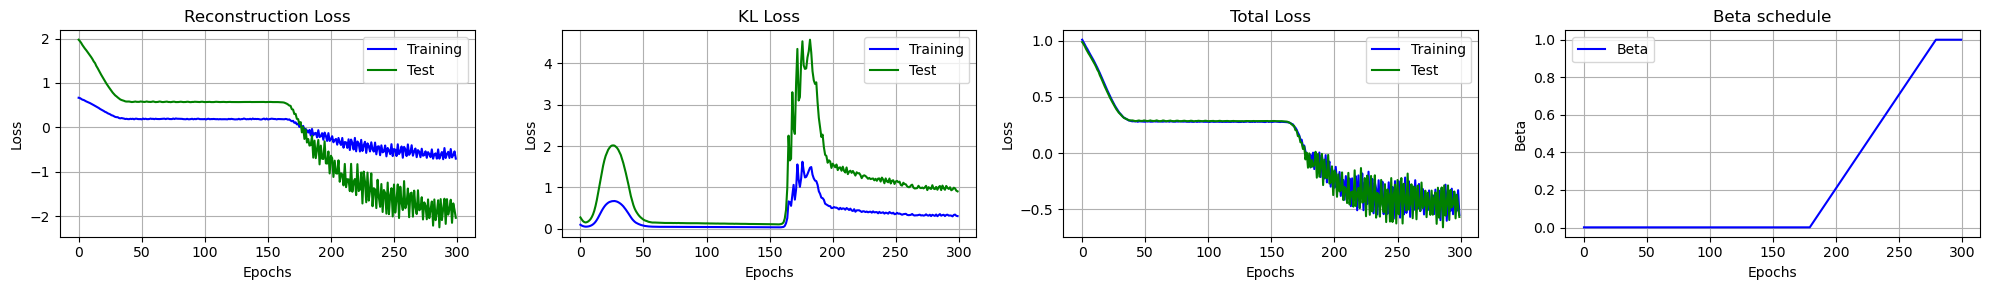
\includegraphics[width=0.9\textwidth]{/home/benjamin/Folders_Python/MVA/MVA_Stage/images/dkf_loss_courbe.png}
    \caption{Training DKF}
    \label{fig:Training DKF}
\end{figure}

The model was able to reconstruct the time-series and generates plausible predictions.

\begin{figure}[H]
    \centering
    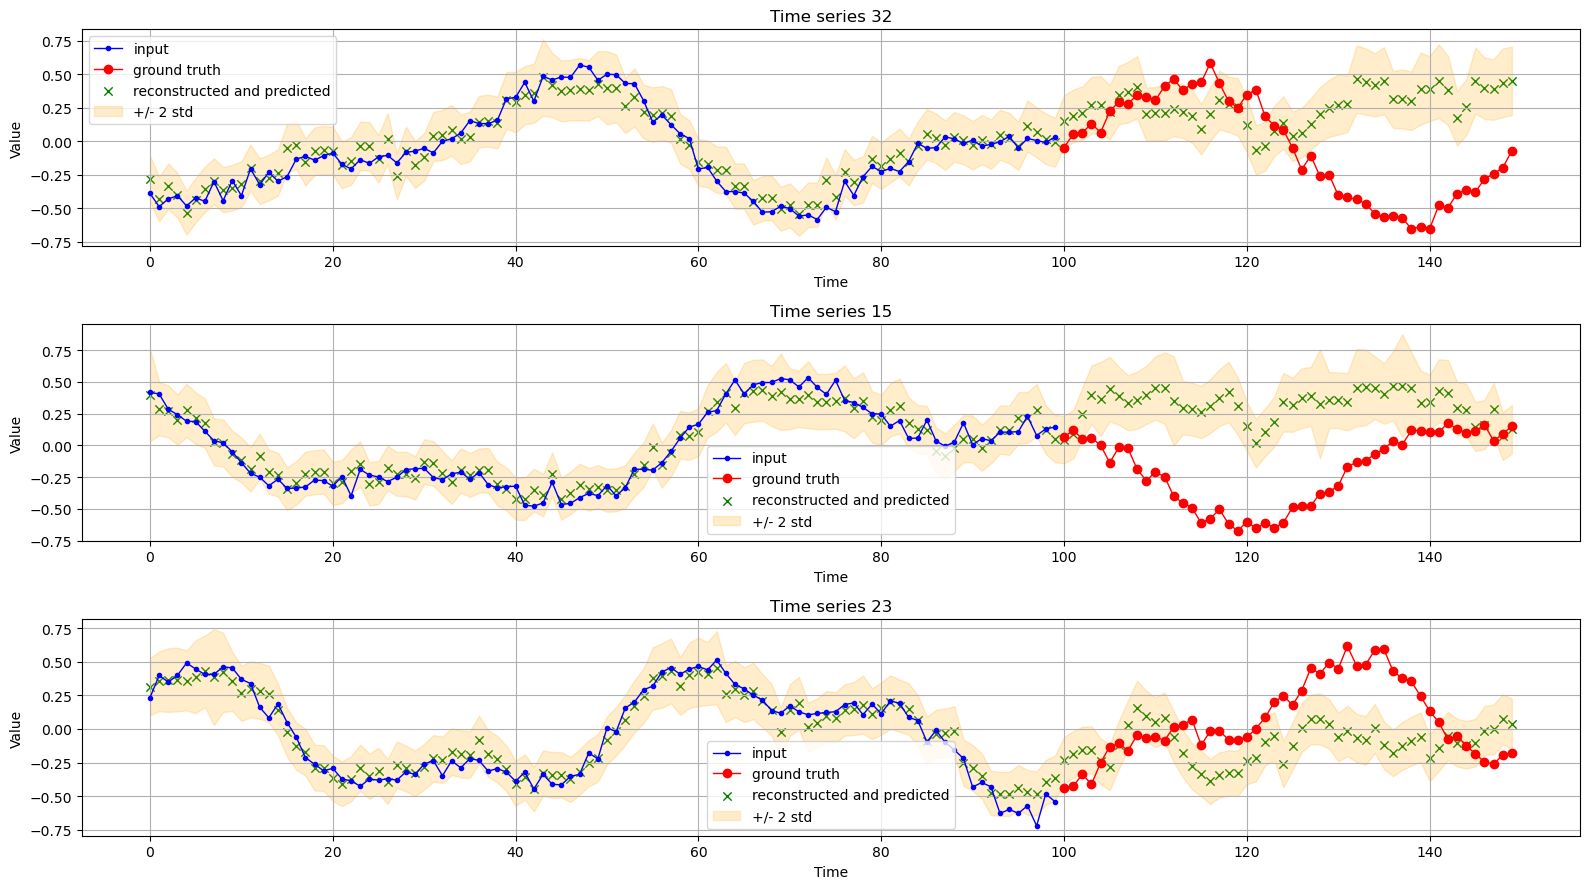
\includegraphics[width=0.9\textwidth]{/home/benjamin/Folders_Python/MVA/MVA_Stage/images/dkf_preds_gens.png}
    \caption{Predictions Generations DKF}
    \label{fig:Predictions Generations DKF}
\end{figure}

\section{Variational Recurrent Neural Network on time series}

We tested a \gls{vrnn} on a toy time serie dataset in
\begin{minted}[frame=single,fontsize=\footnotesize]{python}
Train_VRNN_v1.ipynb
\end{minted}
The time series are shorter than for the \gls{dkf} to reduce training time - thus making the task easier. Results are promising though.

\begin{figure}[H]
    \centering
    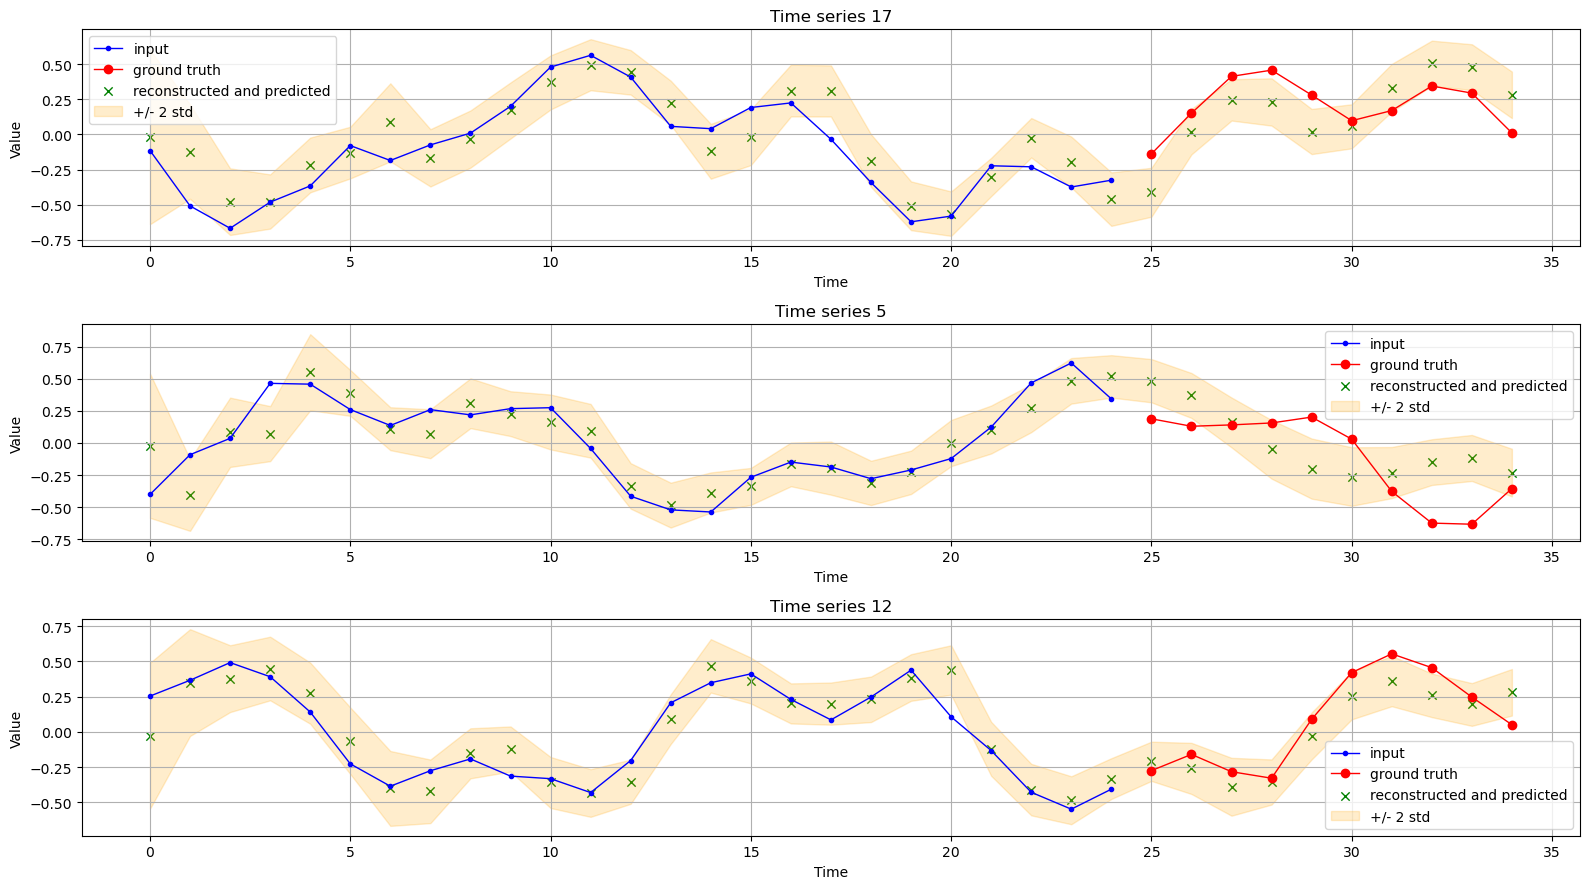
\includegraphics[width=0.9\textwidth]{/home/benjamin/Folders_Python/MVA/MVA_Stage/images/vrnn_toy_time_series.png}
    \caption{Predictions and Generations VRNN}
    \label{fig:Predictions Generations VRNN}
\end{figure}


\section{Sprites Dataset}

We will be using the \textbf{Sprites} dataset from \cite{li_disentangled_2018}.

The Sprites dataset is a synthetic cartoon character dataset of RGB images $64 \times 64 \times 3$. Each character has 4 attributes 
(hair, shoes, top cloth, bottom cloth) that can take 6 possibles values. Each character has three possible poses (left, front, right) 
and can perform 3 possible actions (walk, spell, slash) accross 8 consecutive frames.

There is a total of $6^4 \times 3 \times 3 = 11664$ series of 8 images each, that are divided between a training set and a 
test set.

Here is one character:
\begin{figure}[H]
    \centering
    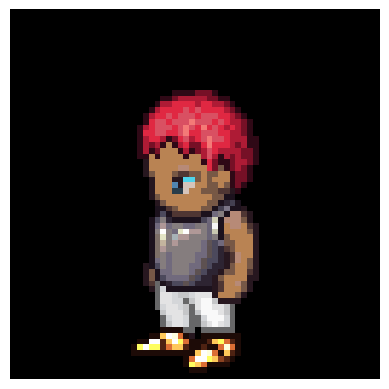
\includegraphics[width=0.4\textwidth]{/home/benjamin/Folders_Python/MVA/MVA_Stage/images/one_sprite.png}
    \caption{One sprite}
    \label{fig:One sprite}
\end{figure}

And 5 series:
\begin{figure}[H]
    \centering
    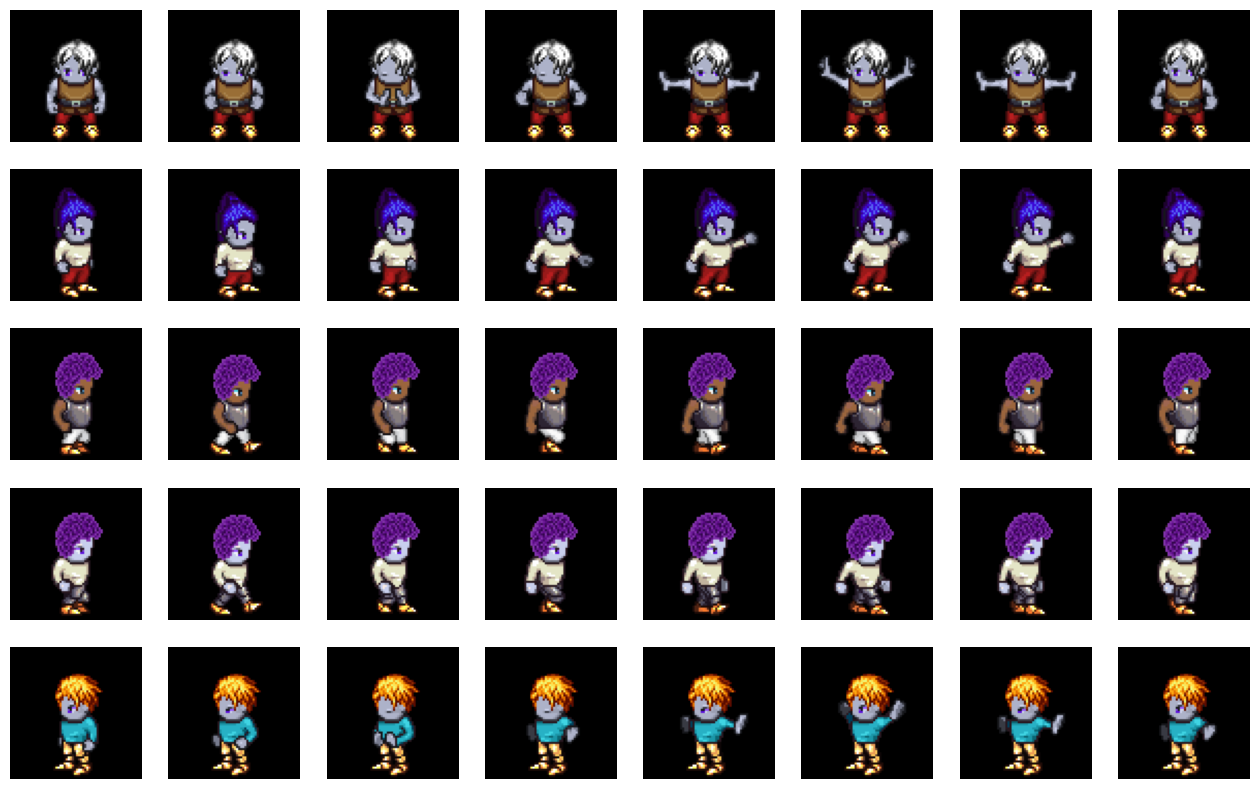
\includegraphics[width=0.9\textwidth]{/home/benjamin/Folders_Python/MVA/MVA_Stage/images/samples_sprites_series.png}
    \caption{sprite series}
    \label{fig:sprite series}
\end{figure}

\section{Variational Recurrent Neural Network}

We trained a \gls{vrnn} in
\begin{minted}[frame=single,fontsize=\footnotesize]{python}
Train_VRNN_Sprites_v1.ipynb
\end{minted}
with a CNN encoder and a CNN decoder. 
The three RNNs of the \gls{vrnn} have a dimension 128, and the latent space dimension is 64.

The training took a little bit more than one hour on a RTX 3090.

The reconstruction is good

\begin{figure}[H]
    \centering
    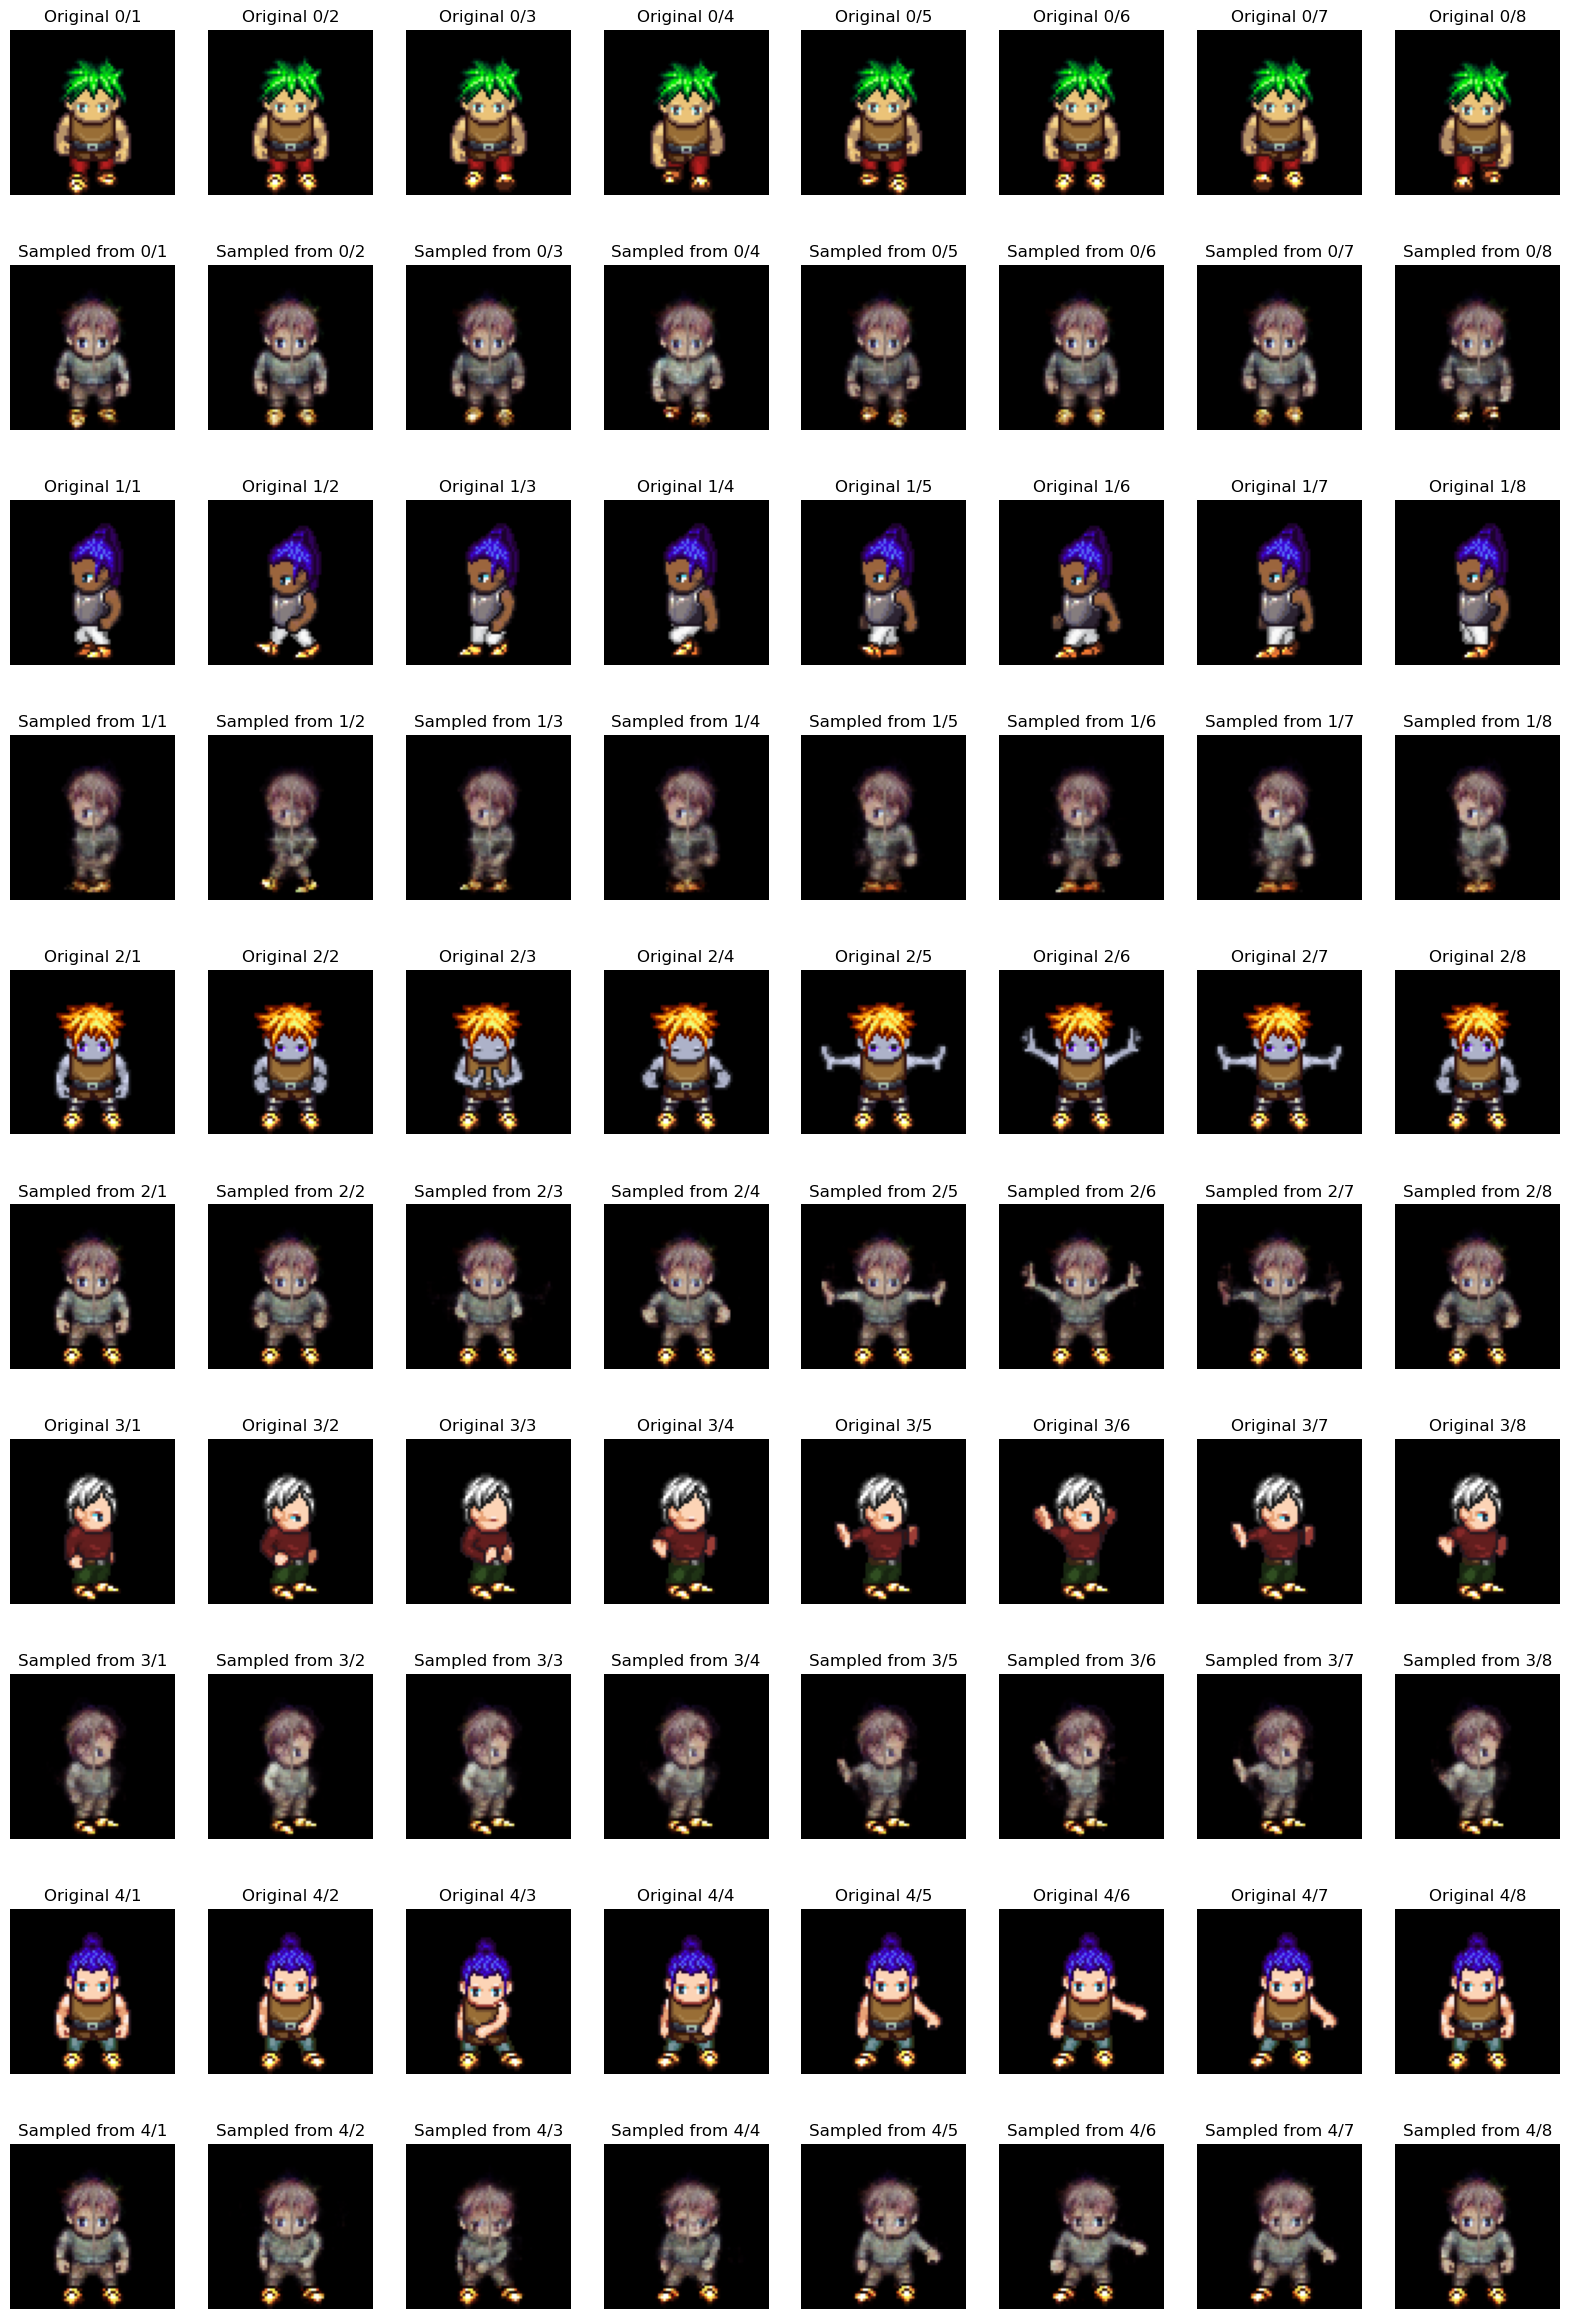
\includegraphics[width=0.9\textwidth]{/home/benjamin/Folders_Python/MVA/MVA_Stage/images/vrnn_sprites_reconstruction.png}
    \caption{VRNN Sprites reconstruction}
    \label{fig:VRNN Sprites reconstruction}
\end{figure}

\newpage
\begin{landscape}
We tested the generation over 20 time steps, with one character as a "seed" to intialize the first latent variable. The model 
can sometimes chain different motions over those 20 steps.

\begin{figure}[H]
    \centering
    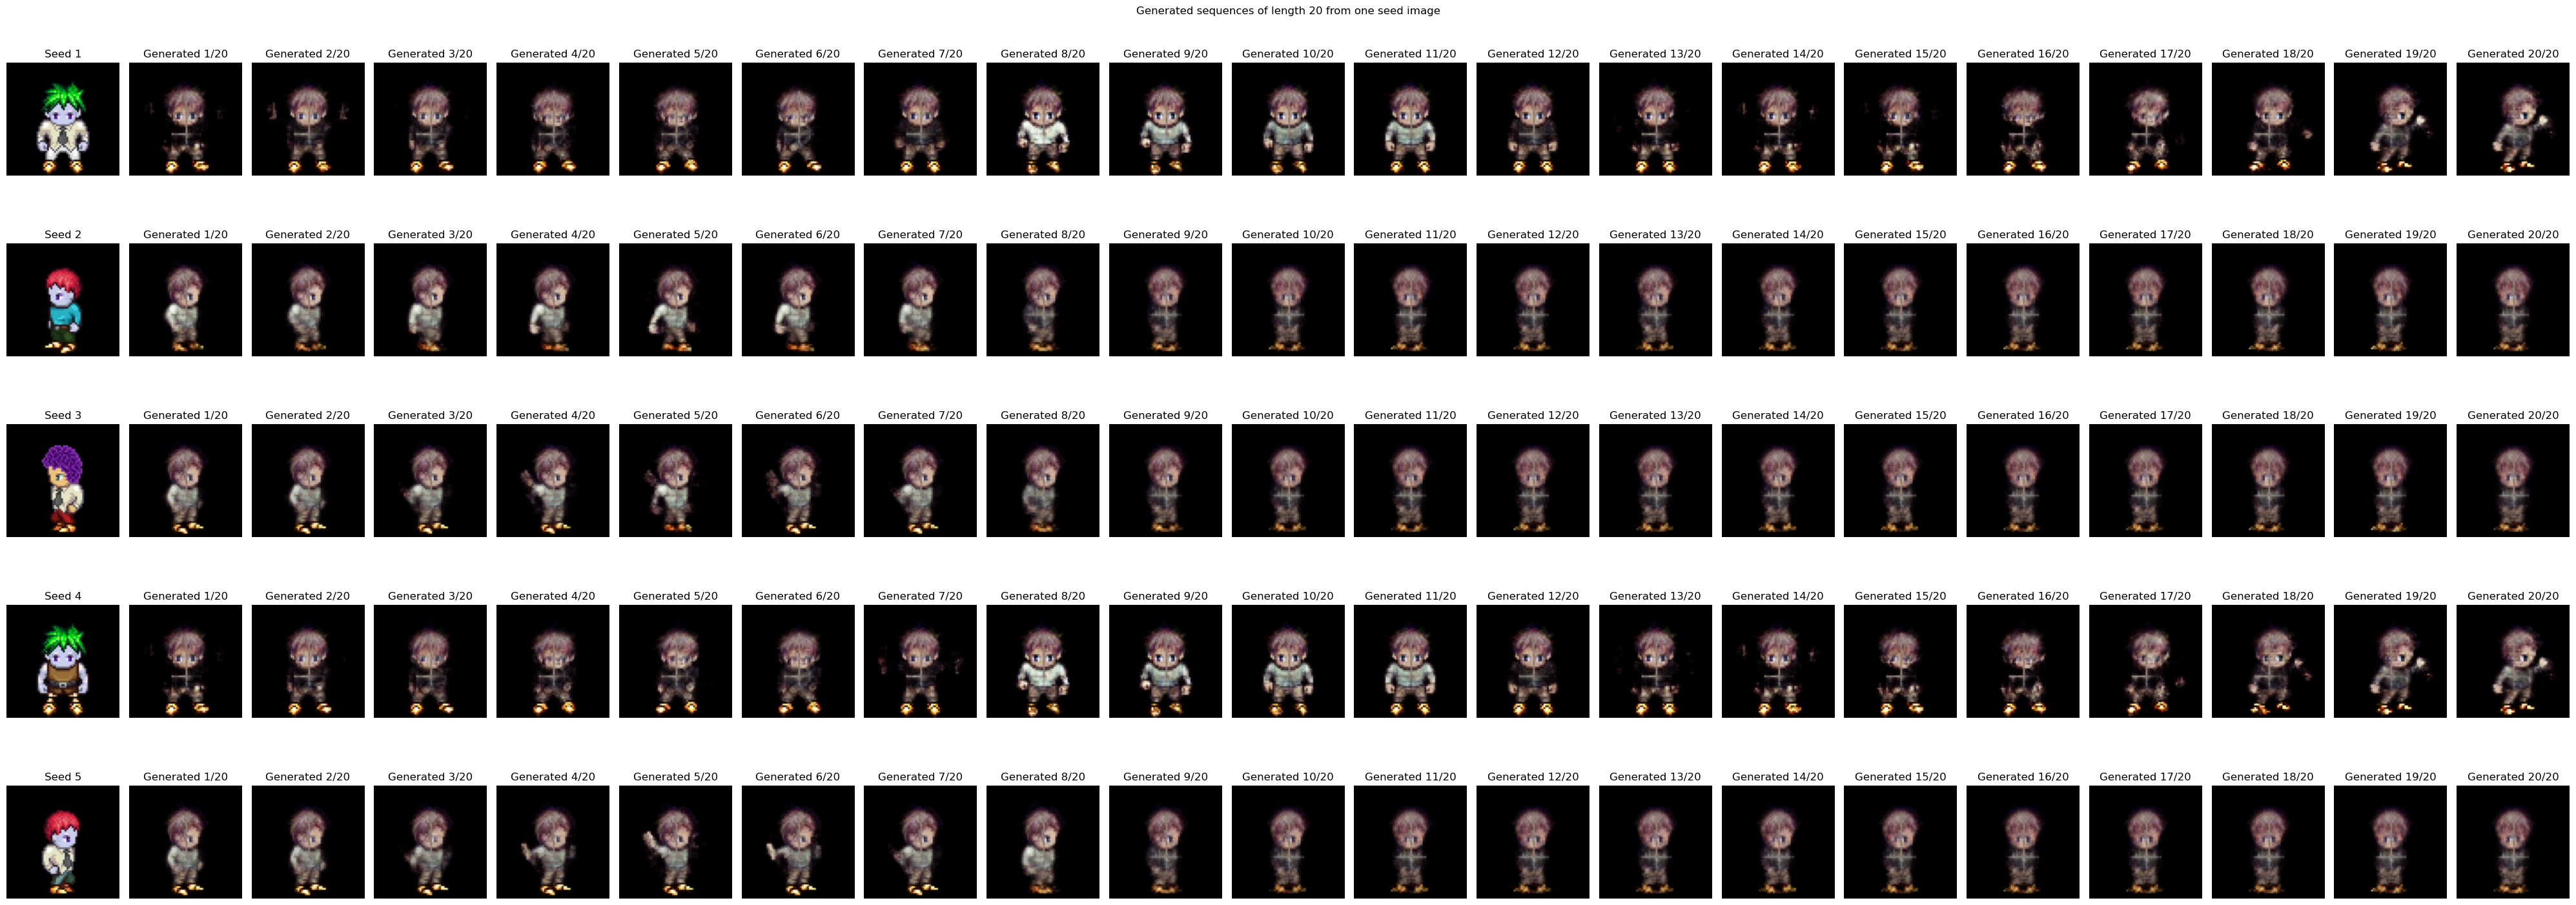
\includegraphics[width=1.3\textwidth]{/home/benjamin/Folders_Python/MVA/MVA_Stage/images/vrnn_sprites_generation.png}
    \caption{VRNN Sprites generation}
    \label{fig:sprite generation}
\end{figure}
\end{landscape}

\section{Gaussian Process Variational Auto Encoder}

The training of the \gls{gpvae} proved challenging.

See the detailed training logic in:
We trained a \gls{vrnn} in
\begin{minted}[frame=single,fontsize=\footnotesize]{python}
Train_GPVAE_step_by_step_logic.ipynb
\end{minted}

The specific notebook for the sprite training is 
\begin{minted}[frame=single,fontsize=\footnotesize]{python}
Train_GPVAE_Sprites_XPs_v2.ipynb
\end{minted}

We coded three different ways of computing a covariance matrix:
\begin{itemize}
    \item covariance matrix
    \item precision matrix
    \item Cholesky decomposition
\end{itemize}

We coded Gaussian kernels and Matern kernels (with $\nu = 0.5, 1.5, 2.5$).
The \mint{python3}|class GaussianKernelFixed| and \mint{python3}|class MaternKernelFixed| have fixed non-trainable lengthscale 
and sigma parameters (sigma is the scaling factor multiplying the kernel).

The \mint{python3}|class GaussianKernel| and \mint{python3}|class MaternKernel| have learnable lengthscale 
and sigma parameters : 
\begin{minted}[frame=single,fontsize=\footnotesize]{python}
self.lengthscale = nn.Parameter(torch.tensor(lengthscale))  # learnable lengthscale parameter    
self.sigma = nn.Parameter(torch.tensor(sigma))  # learnable variance parameter
\end{minted}
However, the attributes must be cloned before being used in the computations to avoid attempts to run multiple backward passes in the 
computation graph and trigger a RunTime Error :
\begin{minted}[frame=single,fontsize=\footnotesize]{python}
lengthscale = self.lengthscale.clone()
sigma = self.sigma.clone()
# ...
kernel = torch.exp(-0.5 * torch.pow(torch.div(t1_b - t2_b, lengthscale),2))  # (..., N, M)
# ...        
gaussian_kernel_matrix = sigma**2 * kernel
\end{minted}

After several tests, we used a total of 32 \glspl{gp} priors of the 4 different kernel types, with different lengthscales:
\begin{minted}[frame=single,fontsize=\footnotesize]{python}
Dz = 32
delta_t = 1.0  # time step between two frames if T=8 frames in [0,1]

kernels_list = [ GaussianKernelFixed(lengthscale=(delta_t / (2**i)), sigma=1.0).to(device) 
for i in range(int(Dz/4)) ] + \
[ MaternKernelFixed(nu=0.5, lengthscale=(delta_t / (2**i)), sigma=1.0).to(device) 
for i in range(int(Dz/4)) ] +  \
[ MaternKernelFixed(nu=1.5, lengthscale=(delta_t / (2**i)), sigma=1.0).to(device) 
for i in range(int(Dz/4)) ] + \
[ MaternKernelFixed(nu=2.5, lengthscale=(delta_t / (2**i)), sigma=1.0).to(device) 
for i in range(int(Dz/4)) ]

mean_functions_list = [ GPNullMean().to(device) for _ in range(Dz) ] # list of Dz identical mean functions
mean, kernel_matrix, L_matrix, p_theta_z = compute_gp_priors(t, Dz, kernels_list, mean_functions_list, 
verbose=True)
\end{minted}

The reconstruction is good, though not perfect. We show here three samples from the reconstructed distribution of three series from the test set. 
\begin{figure}[H]
    \centering
    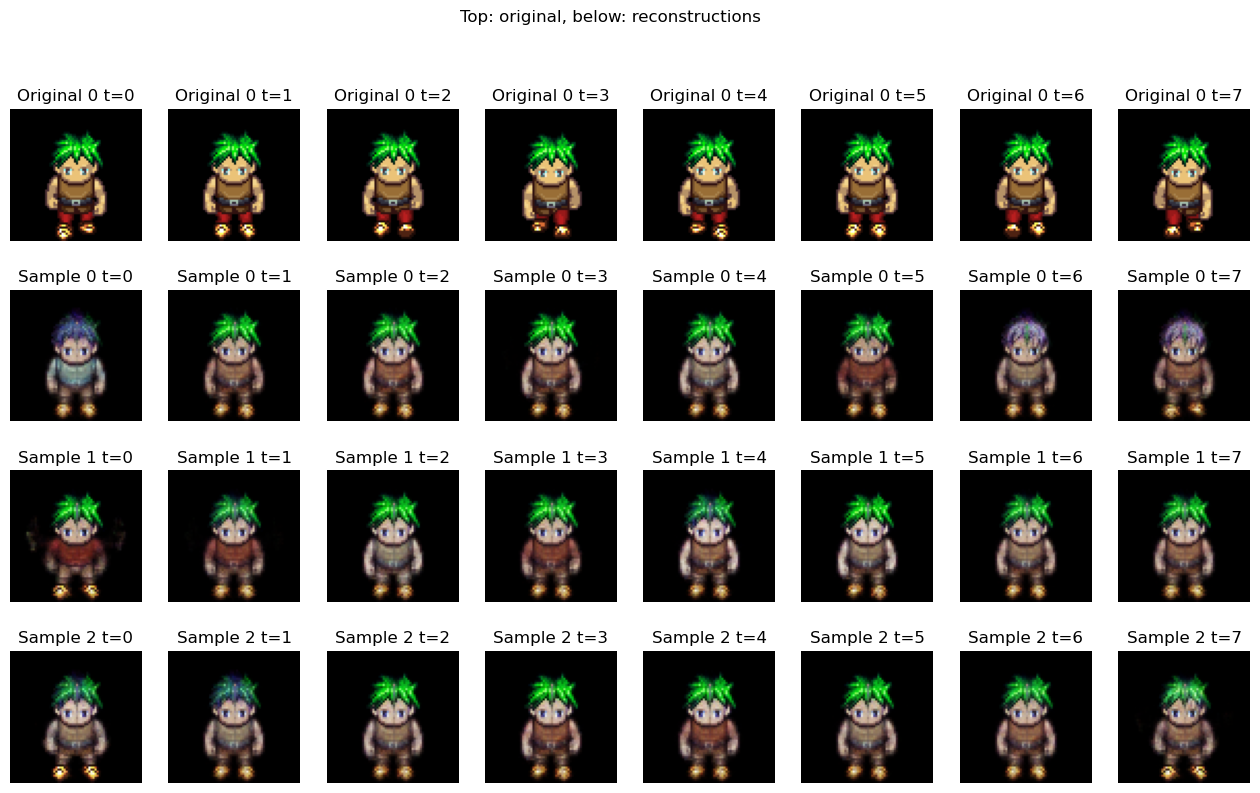
\includegraphics[width=0.9\textwidth]{/home/benjamin/Folders_Python/MVA/MVA_Stage/images/gpvae_reco_01.png}
    \caption{GPVAE Sprites reconstruction 1}
    \label{fig:GPVAE Sprites reconstruction 1}
\end{figure}

\begin{figure}[H]
    \centering
    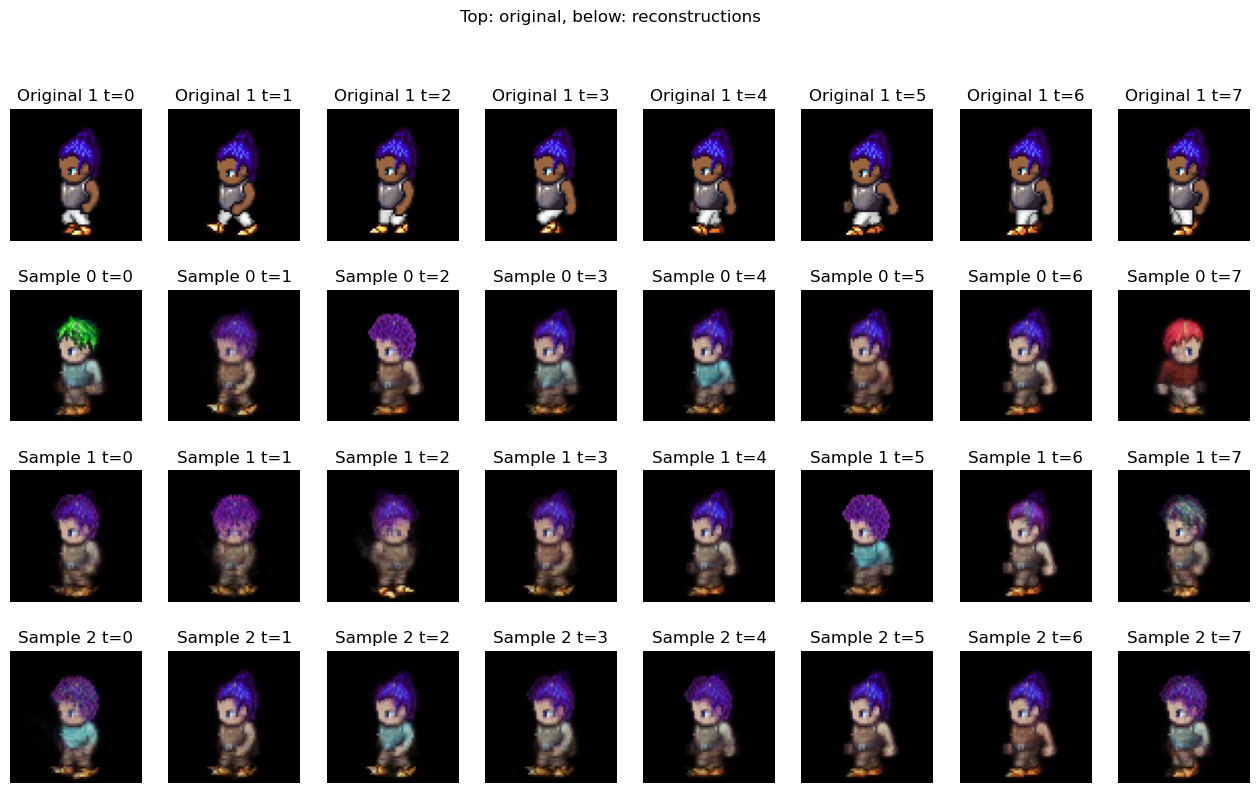
\includegraphics[width=0.9\textwidth]{/home/benjamin/Folders_Python/MVA/MVA_Stage/images/gpvae_reco_02.png}
    \caption{GPVAE Sprites reconstruction 2}
    \label{fig:GPVAE Sprites reconstruction 2}
\end{figure}

\begin{figure}[H]
    \centering
    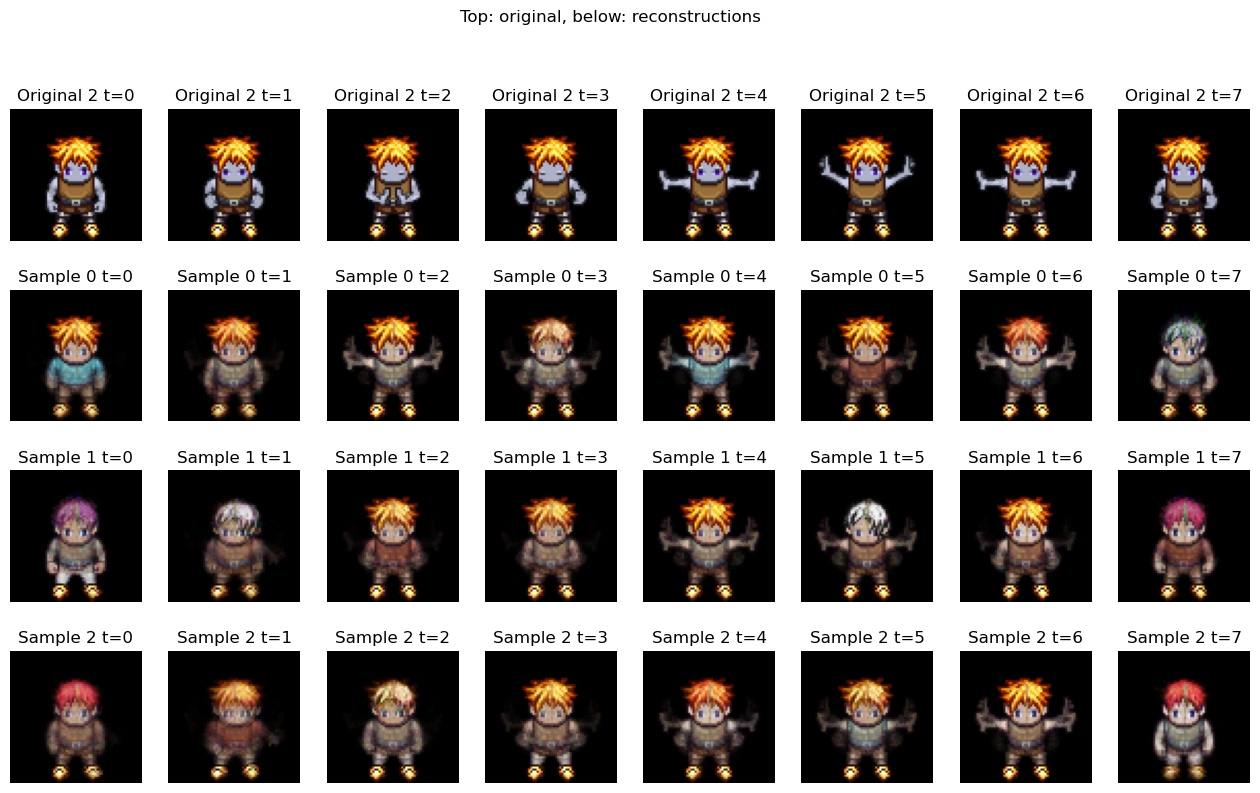
\includegraphics[width=0.9\textwidth]{/home/benjamin/Folders_Python/MVA/MVA_Stage/images/gpvae_reco_03.png}
    \caption{GPVAE Sprites reconstruction 3}
    \label{fig:GPVAE Sprites reconstruction 3}
\end{figure}

The generation is not perfect yet!

\begin{figure}[H]
    \centering
    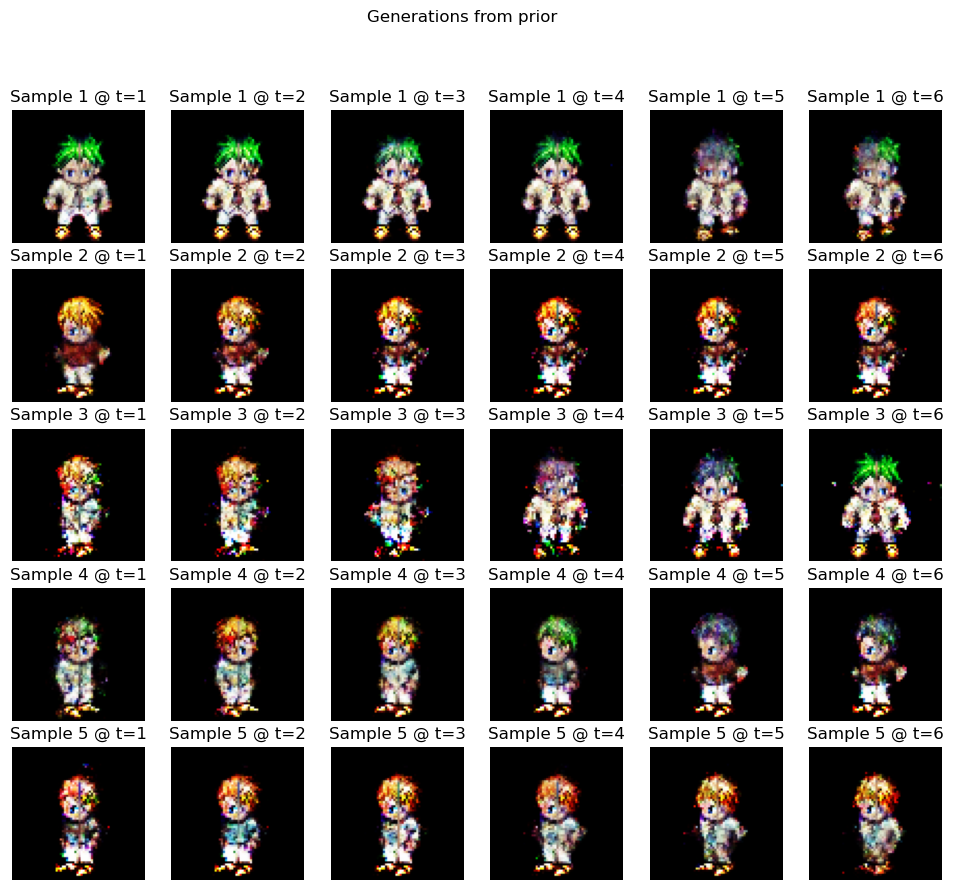
\includegraphics[width=0.9\textwidth]{/home/benjamin/Folders_Python/MVA/MVA_Stage/images/gpvae_gen_01.png}
    \caption{GPVAE Sprites generation 1}
    \label{fig:GPVAE Sprites generation 1}
\end{figure}

In \cite{li_disentangled_2018}, the authors used a Cauchy kernel, whereas we used a mixture of Gaussian and Matern kernels.
This may explain some of our lesser performance.

% 
%
% ------- STOCHASTIC CALCULUS BASICS, SDE AND DVAE ---------------------------
%
%

\part{Notions on stochastic differential equations and their relationships to DVAEs}

This part intends to present a self-contained "survival kit" material on stochastic calculus, in order to highlight the relationships between \glspl{sde} and \glspl{dvae}.

NB : stochastic calculus is a full mathematical field in itself, and a more detailed presentation is located at the very end of this report. For a full study
of the matter, the interested reader will likely enjoy \cite{mouvement-brownien-calcul-ito}, \cite{sarkka_applied_2019}, and refer to \cite{cours-jf-legall}.

    \chapter{Stochastic calculus intoduction}\label{sec:SC_intro}

This chapter is a reminder of some key notions of stochastic calculus. 
More details are presented at the end of the report, and in \cite{mouvement-brownien-calcul-ito}, \cite{sarkka_applied_2019}.

A \textbf{stochastic process} is formally defined as:

\defn{Stochastic process}{
    A stochastic process $X$ is defined as:
\begin{align}
    X &= (\Omega, \mathcal{F}, (X_t)_{t \in T}, \mathbb{P}) \\
    &= (\Omega, \mathcal{F}, (\mathcal{F}_t)_{t \in T}, (X_t)_{t \in T}, \mathbb{P})
\end{align}
where:
    \begin{itemize}
        \item $\Omega$ is a set (universe of possibles).
        \item $\mathcal{F}$ is a $\sigma$-algebra of parts of $\Omega$
        \item $\mathbb{P}$ is a probability measure on $(\Omega, \mathcal{F})$
        \item $T \subset \mathbb{R}_+$ represents time
        \item $(\mathcal{F}_t)_{t \in T}$ is a \textbf{filtration}, ie an increasing family of sub-$\sigma$-algebras of $\mathcal{F}$ indexed by $t$ : $\forall 0 \leq s \leq t \in T$, $\mathcal{F}_s \subset \mathcal{F}_t \subset \mathcal{F}$.
        \item $(X_t)_{t \in T}$ is a family of RV defined on $(\Omega, \mathcal{F})$ with values in a measurable space $(E, \mathcal{E})$ or more simply $(E, \mathcal{B}(E))$ (set $E$ endowed with its Borelian $\sigma$-algebra).
        \item $(X_t)_{t \in T}$ is assumed \textbf{adapted to the filtration} $(\mathcal{F}_t)_{t \in T}$, meaning $\forall t \in T$, $X_t$ is $\mathcal{F}_t$-measurable
    \end{itemize}
}

A filtration $\mathcal{F}_{t\geq 0}$ is often viewed and introduced as the \textit{set of information available at time $t$}. 

The core of stochastic calculus is the stochastic process known as \textbf{Brownian motion}, or \textbf{Wiener process}. 
We use here the definition of a multivariate Brownian motion:

\defn{Brownian motion}{
A stochastic process $B = \brownian$ with values in $\mathbb{R}^d$ is called \textbf{Brownian motion} iff:
\begin{itemize}
    \item $B_0 = 0$ $\mathbb{P}$-a.s.
    \item $\forall 0 \leq s \leq t$, the random variable $B_t-B_s$ is independent from $\mathcal{F}_t$.
    \item $\forall 0 \leq s \leq t$, $B_t - B_s \sim \mathcal{N}(0,Q(t-s))$
    \item $B$ is continuous \footnote{or more exactly there exists a continuous version of $B$, see \cite{mouvement-brownien-calcul-ito}}
\end{itemize}
where the matrix $Q \in \mathbb{S}^{++}_d$ is called the \textbf{diffusion matrix}.
}

Meaning : the process $B$ starts from 0, its increments are independent from the past, its increments over disjoint time intervals are independent of each other, 
its increments follow a centered normal law of variance equal to the length of the time interval multiplied by the diffusion matrix.
NB : some authors choose the define the diffusion matrix (or scalar) outside of the Brownian motion.

A core result is that the quadratic variation of the Brownian motion over an interval $[s,t]$ (equiped
with a subdivison $\pi = \{s=t_0 < t_1 < ...< t_k <... < t_n=t\}$), and defined as the limit when $\vert \pi \vert \rightarrow 0$ 
of $V_{\pi}^{(2)} = \sum_{k=0}^{n-1} \vert f(t_{k+1})-f(t_k)\vert^{2}$, is:

\begin{align}
    &\underset{\vert \pi \vert \rightarrow 0}{\text{lim}}\,\, V_{\pi}^{(2)} = Q(t-s) \,\, \text{in} \,\, L^{2}
\end{align}

Or, heuristically, 
\begin{align}
    \label{dB_square_is_dt}
    \mathbb{E}(dB_t dB_t^T) = Q dt
\end{align}

Ito then proceeds to define \textbf{stochastic integrals}, starting with elementary processes:

\defn{Elementary process}{
A stochastic process $X = (X_s)_{s \in [a,b]}$ is called \textbf{elementary} if there exists a subdivision $a = t_0 < t_1 < ... < t_n = b$ of $[a,b]$, such that:
\[
\forall t \in [a,b], \forall \omega \in \Omega, X_t(\omega) = \sum_{i=0}^{n-1} X_i(\omega) \textbf{1}_{[t_i, t_{i+1}[}(t)
\]
with $\forall i \in \{0,1,..,n-1\}, X_i$ is $\mathcal{F}_{t_i}$-measurable.

This means that, in each interval $[t_i, t_{i+1}[$, $X_t(\omega)$ is independent of $t$ and $X_t(\omega) = X_i(\omega)$.

We define $\mathcal{E}$ (resp. $\mathcal{E}_n, n>0$) the set of all elementary processes on $[a,b]$ (resp. the subset of the $X \in \mathcal{E}$)) such that all $X_i$ have a finite moment $\mathbb{E}X_i <\infty$ (resp $\mathbb{E}(\vert X_i\vert^n) < \infty$
}

\defn{Stochastic integral of an elementary process}{
Let $X \in \mathcal{E}$, ie
\[
X_t(\omega) = \sum_{i=0}^{n-1} X_i(\omega) \textbf{1}_{[t_i, t_{i+1}[}(t)
\]
\textbf{The stochastic integral of $X$ is the real random variable} :
\[
\int_a^b X_t dB_t := \sum_{i=0}^{n-1} X_i (B_{t_{i+1}} - B_{t_{i}})
\]
}

The notion is then extended to other stochastic processes (in spaces of square integrable processes, see the annex).

The definition of a \gls{sde} is derived from the notion of stochastic integral:

\defn{Ito's process}{
    A process $X = (X_t)_{t \in [0, T]}$ is called a \textbf{Ito's process} if it can be written as:
    \begin{align}
        \label{ito sde definition}
        X_t &= X_0 + \int_{0}^{t}a_s ds + \int_{0}^{t} b_s dB_s \,\,\, \forall t \in [0,T]
    \end{align}
    where $a$ and $b$ are two stochastic processes such that the integrals exist (ie $a \in  \Lambda^1$ and 
    $b \in \Lambda^2$).\\
    Equivalently, we write $X_t$ as the soltuion to the \textbf{Stochastic Differential Equation}:
    \begin{align*}
        dX_t = a_t dt + b_t dB_t
    \end{align*}
}

The very famous \textbf{Ito's formula} will allow to make calulations on stochastic processes:

\thmp{Itô's formula}{
An Itô's process remains an Itô's process when it is transformed by a deterministic function that is "smooth enough".

Let $X$ be a Itô's process on $[0,T]$ : $dX_t = a_tdt + b_t dB_t$.

Let:
\begin{align*}
    f : \mathbb{R} \times \mathbb{R} &\rightarrow \mathbb{R} \\
    (x,t) &\mapsto f(x,t)
\end{align*}
be $\mathcal{C}^{2,1}$ : $\mathcal{C}^2$ in $x$, and $\mathcal{C}^1$ in $t$.

Then $(f(X_t,t))_{t \in [0,T]}$ is also an Itô's process and:
\begin{align}
    d\left( f(X_t,t) \right) = \frac{\partial f}{\partial t}(X_t,t) dt + \frac{\partial f}{\partial x}(X_t,t) dX_t + \frac{1}{2}\frac{\partial^2 f}{\partial x^2}(X_t,t)b_t^2 dt
\end{align}
The last term is Itô's complementary term.\\
In dimension $d > 1$:
\begin{align}
    d\left( f(X_t,t) \right) = \frac{\partial f}{\partial t}(X_t,t) dt + ()\nabla f)^T (X_t,t) dX_t + \frac{1}{2}\text{Tr} \left( (\nabla \nabla^T f) dX_t dX_t^T \right)
\end{align}
}{see book \cite{mouvement-brownien-calcul-ito} for a clean proof. A heuristic process can be derived by using a Taylor-Lagrange decomposition at order 2, and using \ref{dB_square_is_dt}}
    \chapter{Stochastic Differential Equations}\label{sec:SDE_results}

We use here the notations of \cite{sarkka_applied_2019} and recall the key results relevant to this report.

\section{Generic SDE}

A generic \textbf{stochastic differential equation} is defined as:

\defn{General Form of a Stochastic Differential Equation}{
    We define a \gls{sde} in dimension $D$.

    Let:
    \begin{itemize}
        \item $B$ be a Brownian motion $B_t \in \mathbb{R}^S$, of diffusion matrix $Q$
        \item $F$ be a deterministic function \textbf{drift} $F : \mathbb{R}^D \times \mathbb{R}\rightarrow \mathbb{R}^{D \times D}$
        \item $L$ be a deterministic function \textbf{diffusion} (or dispersion) $L : \mathbb{R}^D \times \mathbb{R}\rightarrow \mathbb{R}^{D \times S}$ 
    \end{itemize}

    The \gls{sde} is:
    \begin{align}
        \label{generic_sde}
        dX_t &= F(X_t,t) dt + L(X_t,t) dB_t \\
        X_{t_0} &= X_0
    \end{align}
    where $X_0$ can be a scalar constant or a random variable.
    A stochastic process $X$ is said to be solution of \ref{generic_sde} if it verifies:
    \begin{align*}
        \forall t, \,\, X_t = X_0 + \int_{0}^{t} F(X_u, u)du + \int_{0}^{t} L(X_u,u) dB_u
    \end{align*}
}

As for \gls{ode}, a solution to \ref{generic_sde} might not exist. Also, results similar to Cauchy-Lipschitz 
exist for existence and unicity, based on assumptions on $F$ and $L$. 

Intuitively, we can see that an "infinitesimal increment" of $X_t$ to $X_{t+\Delta_t}$ verifies :
$\Delta {X_t} \approx F(X_t, t) \Delta t + L(X_t,t) dB_t$. But $dB_t$ is a Brownian increment independent of $X_{<t}$ (ie $\mathcal{F}_t$),
This suggests that $X_{t+ \Delta_t}$ depends on the past only by $X_t$. In other words, $X_t \vert \mathcal{F}_s = X_t \vert X_s$ 
for any $0 < s < t$. ie : \textbf{the solution of a \gls{sde} is a Markov process}. (The formal proof is given in \cite{mouvement-brownien-calcul-ito}.)

Formally, a Markov process is caracterized by its \textbf{transition kernels}. 
That is, for any $s < t$, and any $A \in \mathcal{B}_{\mathbb{R}^{D}}$, a Markov process verifies 
$\mathbb{P}(X_t \in A \vert \mathcal{F}_s) = \mathbb{P}(X_t \in A \vert X_s)$. And the transition kernels 
of $X$ are the applications $P_{s,t} : \mathbb{R}^{D} \times \mathcal{B}_{\mathbb{R}^{D}} \rightarrow [0,1]$, 
such that for any $f : \mathbb{R}^{D} \rightarrow \mathbb{R}$ measurable and bounded, we have:
\begin{align}
    P_{s,t}f(x) = \int_{{\mathbb{R}^{D}}} P_{s,t}(x,dy) f(y)
\end{align}

So $P_{s,t}$ actually is the probability measure of starting from $x$ at time $s$, and reach $y \in dy$ at time $t$.

When the transition kernels have densities $p(x,t \vert y,s)$ (ie starting from $y$ at time $s$, and
reaching $x$ at time $t$), then a fundamental result is the \textbf{Fokker Plank Kolmogorov} equation 
(also known as forward Kolomogorov) :
\begin{align}
    \label{FPK}
    \frac{\partial p}{\partial y} &= \mathcal{A}^{*}p \\
    \mathcal{A}^{*}(\bullet) &= - \sum_{i=1}^{D} \frac{\partial}{\partial x_i} (F_i(x,t)(\bullet)) + \
        \frac{1}{2} \sum_{i,j=1}^{D} \frac{\partial^{2}}{\partial x_i \partial x_j} (L(x,t)QL(x,t)^{T}\vert_{i,j} (\bullet))
\end{align}


The Fokker-Plank-Kolmogorov equation \ref{FPK} allows to derive -ordinary- differential equations for the moments 
of $X_t$ (see \cite{sarkka_applied_2019}). For the first two, defining
\begin{align}
    m(t) &= \mathbb{E}(X_t) \\
    P(t) &= \mathbb{E}((X_t - m(t))(X_t-m(t))^{T})
\end{align}

We have (NB : the expectations are taken w.r.t. $x$, ie the density probability $(p(x,t))$) :
\begin{align}
    \label{SDE_moments}
    \frac{dm}{dt} &= \mathbb{E}(F(x,t)) \\
    \frac{dP}{dt} &= \mathbb{E}(F(x,t)(x-m(t))^{T}) + \mathbb{E}((x-m(t)) F(x,t)^{T}) +\
    \mathbb{E}(L(x,t)QL(x,t)^{T})
\end{align}


\section{Linear SDE}

A particularly useful flavor of \gls{sde} is the linear \gls{sde}, that allows some close-form (or at least nicer) solutions:

\defn{Linear Stochastic Differential Equation}{
    With the same notaions as \ref{generic_sde}:

    The linear \gls{sde} is:
    \begin{align}
        \label{linear_sde}
        dX_t &= F(t) X_t dt + L(t) dB_t \\
        X_{t_0} &= X_0 \sim \mathcal{N}(m_0, P_0)
    \end{align}
}

In this case, the transition kernels family can be characterized as:
\begin{align}
    \Psi &: \mathbb{R}^{2 } \rightarrow \mathbb{R}^{D} \\
    \frac{\partial \Psi (\tau, t)}{\partial \tau} &= F(\tau) \Psi(\tau, t) \\
    \frac{\partial \Psi (\tau, t)}{\partial t} &= - \Psi(\tau, t) F(t)  \\
    \Psi(\tau, t) &= \Psi(\tau, s) \Psi(s, t) \,\,\, (\text{Chapman-Kolmogorov}) \\
    \Psi(\tau, t) &= \Psi(t, \tau)^{-1} \\ 
    \Psi(t,t) &= I_d
\end{align}

And:
\prop{the solution to \ref{linear_sde} is:
\begin{align}
    \label{solution_linear_sde}
    X_t &= \Psi(t,t_0) X_0 + \int_{t_0}^{t} \Psi(t, \tau) L(\tau) dB_{\tau} \\
    X_{t_0} &= X_0
\end{align}
}

If $F$ is constant, we find : $X_t = \exp{F(t-t_0)}X_0 + \int_{t_0}^{t} \exp{F(t- \tau)}L(\tau)dB_{\tau}$

We see from the form of \ref{solution_linear_sde} that, when $X_0$ is Gaussian, then $X_t$ is a linear combination of 
independent Gaussian random variables, therefore Gaussian. ie : \textbf{the solution of a linear SDE is a Gaussian process}. 
(NB: the converse is NOT true)

In this case, the first two moments of $X_t$ are enough to fully describe the solution. The equations \ref{SDE_moments} simplify into:
\begin{align}
    \label{SDE_linear_moments}
    \frac{dm}{dt} &= F(t) m(t) \\
    \frac{dP}{dt} &= F(t)P(t) + P(t)F(t)^{T} + L(t)QL(t)^{T} \\
    \text{with initial condition } \,\, X_0 &\sim \mathcal{N}(m_0, P_0)
\end{align}
The transition density ($p(X_t = x(t) \vert X_s = x(s)$) can be found explicitely ($0 < s < t$):
\begin{align}
    p(x_t \vert x_s) &= \mathcal{N}(x_t \vert m(t\vert s), P(t \vert s)) \\
    m(t \vert s) &= \Psi(t,s)x(s) \\
    P(t \vert s) &= \int_{s}^{t} \Psi(t,\tau)L(\tau)Q L(\tau)^{T}\Psi(t, \tau)^{T} d\tau
\end{align}

Which allows to \textbf{discretize} the \gls{sde} as:
\begin{align}
    \label{linear sde discretization}
    x_{t_{k+1}} &= A_k x_{t_k} + q_k \\
    q_k &\sim \mathcal{N}(0, \Sigma_k) \\
    A_k &= \Psi(t_{k+1}, t_k) \\
    \Sigma_k &= \Sigma(t_{k+1}, t_k) = \int_{t_k}^{t_{k+1}} \Psi(t_{k+1}, \tau) L(\tau)Q L(\tau)^{T} \Psi(t_{k+1}, \tau)^{T} d\tau
\end{align}

In practice, the \textbf{linearization of an SDE} is one of the techniques used to approximate \gls{sde} and 
allow computations:
\begin{align}
    dX_t &= F(X_t, t)dt + L(X_t, t)dB_t \\
    F(X_t, t) &\approx F(m(t), t) + J_X F(m(t),t)(X_t - m(t)) \\
    L(X_t, t] &\approx L(m(t),t) \\
    \frac{dm}{dt} &= F(m(t), t) \\
    \frac{dP}{dt} &= J_X F(m(t),t) P(t)^{T} + P(t)J_X F(m(t),t)^{T} + L(m(t), t)QL(m(t),t)^{T} \\
\end{align}
where $J_X F$ is the Jacobian of $F$ w.r.t $X$.

A set of example calculations for the Ornstein-Uhlenbeck process is located in the appendix.
    % add chapter for links between SDEs and DVAEs
    \chapter{Filtering, Smoothing, and the Kernels Zoo}\label{sec:filter smoother gps}

Equiped with the stochastic calculus basics, we see in this chapter that the filtering and smoothing 
tasks (ie computing posterior probabilities of the latent variables) provides a complete framework 
for the corresponding tasks in \glspl{dvae}.

We also see that, when a Gaussian process can be formulated as the solution of a linear \gls{sde} (ie
 when the kernel function verifies some properties), then the gaussian process regression problem 
 of computing posterior probabilities can be performed by algorithms in linear time.

In this chapter, we consider \glspl{ct-ssm} and \glspl{cd-ssm}. In both cases, the latent variables are 
defined by a (continuous) \gls{sde}. The observations can be defined by a second \gls{sde}, or by a set of 
discrete-time observations.

Formally, the \gls{ct-ssm} is defined by:

\begin{tcolorbox}[colback=blue!5!white,colframe=black!75!black,title=Continuous-Time State Space model]
    \begin{align}
        dZ_t &= F(Z_t, t)dt + L(Z_t,t) dB_t \\
        dX_t &= H(Z_t,t)dt + d\eta_t
    \end{align}
    where:
    \begin{itemize}
        \item $Z_t \in \mathbb{R}^{D}$ is the \textit{state}, ie a stochastic process defining the latent variable.
        \item $B_t \in \mathbb{R}^{S}$ is a Brownian motion with diffusion matrix $Q$.
        \item $F \in \mathbb{R}^{D}$ and $L \in \mathbb{R}^{D \times S}$ are the usual drift and dispersion functions.
        \item $X_t \in \mathbb{R}^{M}$ is the \textit{integrated} measurement (or observation) process.
        \item $H \in \mathbb{R}^{M}$ is the observation/measurement model.
        \item $\eta_t \in \mathbb{R}^{S}$ is a Brownian motion with diffusion matrix $R$.
    \end{itemize}
    NB : the observations are assumed to conditionnally independent of the state, and $B_t, \eta_t$ are 
     assumed independent.
    The observation model is equivalent to:
    \begin{align}
        y_t &= \frac{dX_t}{dt} = H(Z_t,t) + \epsilon_t \\
        \epsilon_t &= \frac{d \eta_t}{dt}
    \end{align}
\end{tcolorbox}

Formally, the \gls{cd-ssm} is defined by:

\begin{tcolorbox}[colback=blue!5!white,colframe=black!75!black,title=Continuous-Discrete State Space model]
    \begin{align}
        dZ_t &= F(Z_t, t)dt + L(Z_t,t) dB_t \\
        x_k &\sim p(x_k \vert z_{t_k})
    \end{align}
    where:
    \begin{itemize}
        \item $Z_t \in \mathbb{R}^{D}$ is the \textit{state}, ie a stochastic process defining the latent variable.
        \item $B_t \in \mathbb{R}^{S}$ is a Brownian motion with diffusion matrix $Q$.
        \item $F \in \mathbb{R}^{D}$ and $L \in \mathbb{R}^{D \times S}$ are the usual drift and dispersion functions.
        \item $x_k$ are the observations taken at \textbf{discrete times $(t_k)_{k=1,...,n}$}
    \end{itemize}
    NB : the observations are assumed to conditionnally independent of the state.
\end{tcolorbox}

We see that the \gls{gpvae} is a specific \gls{cd-ssm}, where the underlying latent stochastic process 
is actually a Gaussian process.

Also, the \gls{ct-ssm} assumes a Gaussian observation model, whereas the \gls{cd-ssm} allows more general 
observation models.

From a vocabulary stand-point, we will use indifferently \textit{state} or \textit{latent variable}, and 
\textit{observation} or \textit{measurement}.

\section{Filtering and Smooting}

\textbf{Filtering} is the problem of determining the posterior probability of the latent $Z_t$ given the 
discrete measurements, ie finding $p(Z_t \vert x_{1:k})$ with $t_k \leq t$. This corresponds to 
determining the generative transition probability $p_{\theta_z}(z_t \vert z_{1:t-1}, x_{1:t-1})$ in our 
\gls{dvae} setting.

\textbf{Smoothing} is the problem of determining the posterior probability of the latent $Z_t$ given 
all known observations, ie finding $p(Z_t \vert x_{1:T})$ for all $t \in [0,T]$. This corresponds to 
determining the inference model $q_{\phi}(z_t \vert z_{1:t-1}, x_{1:T})$ in the \gls{dvae} setting.

In general, close-form solutions can be derived when the latent variables \gls{sde} is linear. In continuous 
time, we get the \textbf{Kalman-Bucy} filter equations, which discretize in the well-known \textbf{Kalman filter}.

\begin{tcolorbox}[colback=blue!5!white,colframe=black!75!black,title=Kalman-Bucy filter]
    
\end{tcolorbox}

\part{Perspective and conclusion}

    \chapter{Latent ODE and SDE models}\label{sec:Latent ODE and SDE models}

\section{Latent ODE models}

\glspl{latent ode} is a class of models introduced in \cite{chen_neural_2019} : "Neural Ordinary Differential Equations" 
by Ricky T. Q. Chen, Yulia Rubanova, Jesse Bettencourt, David Duvenaud. 
ArXiV : \href{https://arxiv.org/abs/1806.07366}{Neural ODE Best Paper Award NeurIPS 2018}.\\

The starting point is to write the evolution of the latent state $z_t$ as:
\begin{align}
    z_{t+1} &= z_t + f(z_t, \theta_t)
\end{align}
where $z_t \in \mathbb{R}^D$ is the latent state, $\theta_t$ is a set
 of parameters at time $t$, and $f$ is a function.

This formulation is the one used in ResNet blocks, and can be 
seen as the Euler transformation of a continuous transformation.

Taking the expression to the limit as $dt \rightarrow 0$, we can write an 
\gls{ode}:
\begin{align}
    \frac{dz_t}{dt} &= f(z_t, t, \theta_f)
\end{align}
where $\theta_f$ is a set of parameters, that can typically be the parameters of 
a neural network learning $f$.

For a time series $x_{t_1}, x_{t_2}, ... x_{t_N}$, Chen and al. in \cite{chen_neural_2019} 
assume the following generative model:
\begin{align}
    z_{t_0} &\sim p_{\theta_z}(z_{t_0}) \\
    z_{t_1}, z_{t_2}, ..., z_{t_N} &= \text{ODE Solver}(z_{t_0}, f, \theta_f, t_0, ..., t_N ) \\
    x_{t_i} &\sim p_{\theta_x}(x_t \vert z_t)
\end{align}
We note that the latent variable is stochastic only through its initial state $z_{t_0}$. 
The evolution of $z_t$ is then deterministic through the \gls{ode}.

The inference model is:
\begin{align}
    [\mu_\phi, \Sigma_\phi] &= \text{LSTM} (x_{t_0:t_N})   \\
    q_{\phi}(z_{t_0} \vert x_{t_0:t_N}) &= \mathcal{N}(z_{t_0} \vert \mu_{\phi}, \Sigma_\phi)
\end{align}

We reproduce here the drawing from the paper:

\begin{figure}[H]
    \centering
    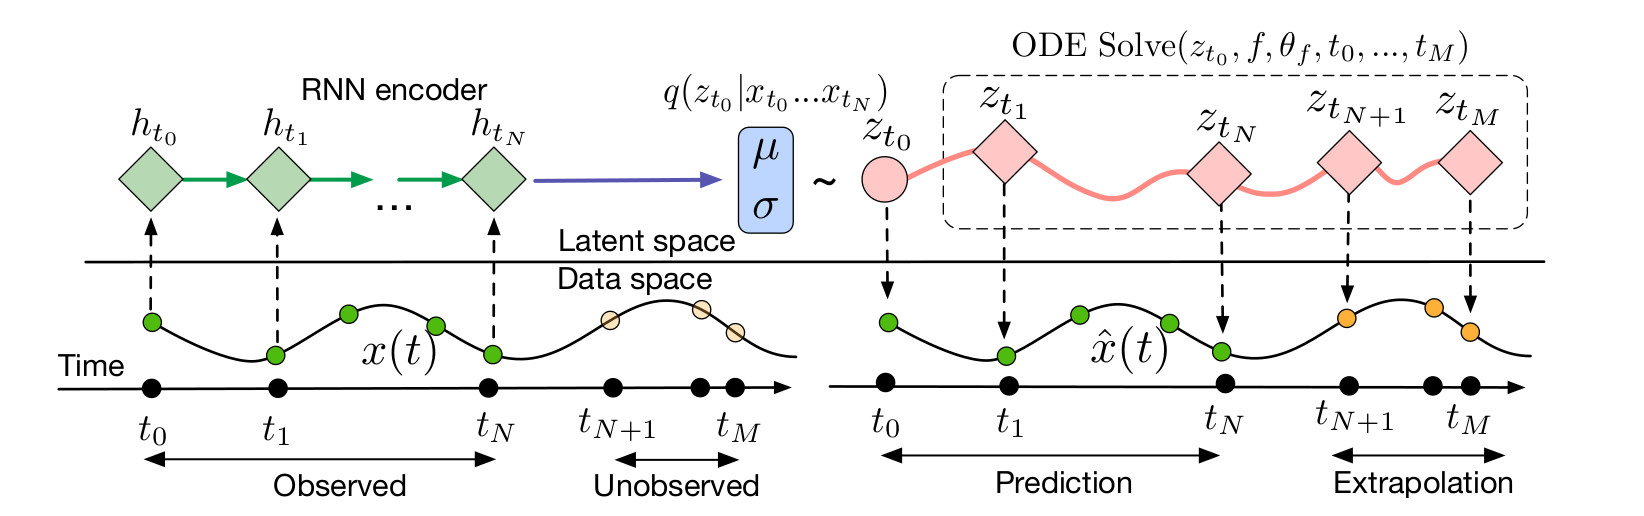
\includegraphics[width=0.9\textwidth]{/home/benjamin/Folders_Python/MVA/MVA_Stage/images/Neural_ODE_01.png}
    \caption{Latent ODE model}
    \label{fig:Latent ODE model}
\end{figure}

The model is trained maximizing a \gls{vlb} as usual. 

Here, the stochastic variables are $z_{t_0}$ and the $x_{t_i}$, the joint distribution writes:
\begin{align}
    p(x_{t_1:t_N}, z_{t_0}) &= p(z_{t_0})p(x_{t_1:t_N} \vert z_{t_0}) \\
    &= p(z_{t_0}) \prod_{t=1}^{N}p_{\theta_x}(x_{t_i} \vert z_{t_i})
\end{align}
And the likelihood:
\begin{align}
    p(x_{t_1:t_N}) &= \frac{p(x_{t_1:t_N}, z_{t_0})}{p(z_{t_0} \vert x_{t_1:t_N})} \\
    \log{p(x_{t_1:t_N})} &= \mathbb{E}_{q_{\phi}(z_{t_0} \vert x_{t_1:t_N})} \log{\frac{p(x_{t_1:t_N}, z_{t_0})}{q_{\phi}(z_{t_0}\vert x_{t_1:t_N})}\frac{q_{\phi}(z_{t_0}\vert x_{t_1:t_N})}{p(z_{t_0} \vert x_{t_1:t_N})}}
\end{align}
The \gls{vlb} is:
\begin{align}
    \log{p(x_{t_1:t_N})} &\geq \mathbb{E}_{q_{\phi}(z_{t_0} \vert x_{t_1:t_N})} \log{\frac{p(x_{t_1:t_N}, z_{t_0})}{q_{\phi}(z_{t_0}\vert x_{t_1:t_N})}} \\
    &= \mathbb{E}_{q_{\phi}(z_{t_0} \vert x_{t_1:t_N})} \log{\frac{p(z_{t_0}) \prod_{t=1}^{N}p_{\theta_x}(x_{t_i} \vert z_{t_i})}{q_{\phi}(z_{t_0}\vert x_{t_1:t_N})}} \\
    &= \sum_{i=1}^{N} \mathbb{E}_{q_{\phi}(z_{t_0} \vert x_{t_1:t_N})} \log{p_{\theta_x}(x_{t_i} \vert z_{t_i})} - \mathbb{KL}(q_{\phi}(z_{t_0} \vert x_{t_1:t_N}) \vert\vert p(z_{t_0}))
\end{align}
With the simple prior $p(z_{t_0}) = \mathcal{N}(0,1)$.

Optimizing the \gls{vlb} requires that we compute the gradients on $\log{p_{\theta_x}(x_{t_i} \vert z_{t_i})}$ w.r.t. $\theta_f$, as the $z_{t_i}$ are solutions of the \gls{ode} depending 
on $f$ and its set of parameters $\theta_f$. One method is the \textbf{adjoint sensitivity method} described in \cite{pontriagin_mathematical_2018}, 
and that the interested reader will find a proof sketch in the appendix \ref{sec:adjoint_sensitivity_method}. Other methods exist, can be reviewed in \cite{sengupta_efficient_2014}.

\section{Latent SDE models}

\glspl{latent ode} models have limitations :
\begin{itemize}
    \item the latent dynamic is deterministic by design
    \item the intial variable $z_{t_0}$ encompasses the entire randomness of the prior, and can become
    unnaturally large to account for randomness along the entire timeline
\end{itemize}

The idea in \cite{li_scalable_2020} is then to add some noise to the deterministic computation of the latent variable:
\begin{align}
    \frac{dz_t}{dt} &= f_{\theta_f}(z_t,t) + \epsilon_t \\
    \epsilon_t &\sim \mathcal{N}(0,Q \textit{Id})
\end{align}
Which leads to an \gls{sde} prior:
\begin{align}
    \label{latent sde prior}
    dZ_t &= f_{\theta}(Z_t, t)dt + \sigma_{\theta}(Z_t,t)dB_t \\
    Z_{t_0} &\sim Z_0
\end{align}
where we used $\sigma_{\theta}$ insted of our usual $L(Z_t,t)$ to stick to the notations of the paper.

\ref{latent sde prior} defines a prior distribution over functions. In order to draw a sample function, we would:
\begin{itemize}
    \item draw a sample $z_{t_0} \sim Z_0$
    \item draw a random Brownian motion $\tilde{B_t}$ path from $B_t$
    \item compute $z_t - z_{t_0} = \int_{t_0}^{t} f_{\theta}(Z_t, t)dt + \int_{t_0}^{t} \sigma_{\theta}(Z_t,t)d\tilde{B_t}$
\end{itemize}

We will use neural networks to learn the drift $f_{\theta}$ and the diffusion $\sigma_{\theta}$, which requires that we are able to compute the gradient of 
a functional (loss) of type:
\begin{align}
    L(\theta) &= L \left( \int_{t_0}^{t_1} f_{\theta}(Z_t, t)dt + \int_{t_0}^{t} \sigma_{\theta}(Z_t,t)dB_t \right)
\end{align}
where $\int_{t_0}^{t} \sigma_{\theta}(Z_t,t)dB_t$ is actually a random variable!

It appears that the adjoint sensitivity method can be adapted to SDEs (see \cite{li_scalable_2020}).

The approximate posterior can also be described as a \gls{sde}:
\begin{align}
    dZ_t &= f_{\phi}(Z_t,t)dt + \sigma_{\phi \, = \, \theta}(Z_t,t)dB_t \\
    Z_{t_0} &= z_0 \, \text{from prior}
\end{align}
where:
\begin{itemize}
    \item the prior and the approximate posterior share the same diffusion for the $\mathbb{KL}$ to have the same support
    \item the prior and the approximate posterior have the same starting value $z_0$
\end{itemize}

We reproduce the model from the paper:

\begin{figure}[H]
    \centering
    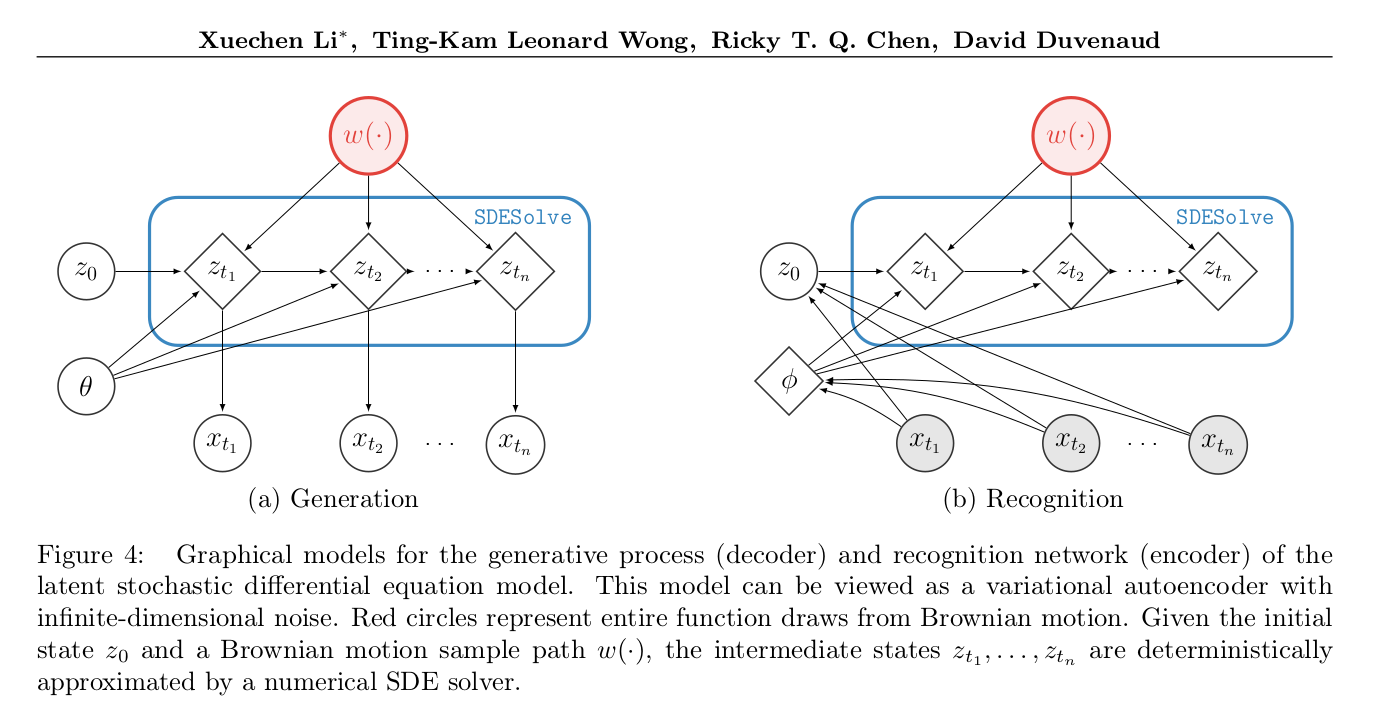
\includegraphics[width=0.9\textwidth]{/home/benjamin/Folders_Python/MVA/MVA_Stage/images/Latent_SDE_01.png}
    \caption{Latent SDE model}
    \label{fig:Latent SDE}
\end{figure}

The stochastic \gls{vlb} writes:
\begin{align}
    \mathcal{L}(\theta, \phi, x_{1:T}) &= \mathbb{E} \left(
        \frac{1}{2}\int_{0}^{T} \vert \frac{f_{\theta}(z_t,t) - f_{\phi}(z_t,t)}{\sigma_{\theta}(z_t,t)}dt \vert^{2} - 
        \sum_{i=1}^{N} \log{p_{\theta_x}}(x_{t_i} \vert z_{t_i})
        \right)
\end{align}

    \chapter{Conclusions}\label{sec:Conclusion}

We have seen that \glspl{vae} can be applied to data sequences by assuming a temporal relationship in the prior over latent variables. 
This is the framework of \glspl{dvae}. When the prior over the latent variables is discrete, this formulation produces, for example, 
\gls{dkf} and \gls{vrnn}, which we detailed, coded and tested on two toy datasets.

Assuming a continuous-time prior over the latent variables provides more expressiveness, as it can handle irregularly sampled data. 
A first model is \gls{gpvae} in which the latent prior is a set of \glspl{gp} over the time dimensions. We detailed, coded and tested 
the \gls{gpvae} on the Sprites dataset. If this model is potentially more expressive than its discrete counterparts, it is also 
tricker to train, as the choice of prior reverts to a choice of kernel functions.

Factoring in stochastic calculus opens a broader perspective and a new field of models. \glspl{gp} include stochastic processes 
solutions to linear \glspl{sde} and allow to use linear-time filtering and smoothing algorithms to reduce computation times. 

The Markovian nature of stochastic processes solutions of general \glspl{sde} allows to use \glspl{sde} to formulate latent priors 
that are suitable for filtering and smoothing. This idea of \glspl{latent sde} builds on \glspl{latent ode} and points to a 
set of potentially very expressive models.

It's been quite a personal journey... and it continues.

%
%
% ----- STOCHASTIC CALCULUS IN DETAILS ---------------------
%
%

\part{Complements}

    \chapter{Stochastic processes main theory}\label{sec:Stochastic_Processes}
    
% \section{Definition and properties of a stochastic process}

We posit the following in the rest of the doc, unless specified otherwise:
% \begin{tcolorbox}[colback=blue!5!white,colframe=black!75!black,title=]
\asum{Main assumptions}{
\begin{enumerate}
    \item $(\Omega, \mathcal{F}, \mathbb{P})$ is a probabilistic space, with $\Omega$ the universe, $\mathcal{F}$ the tribe ($\sigma$-algebra) of events, $\mathbb{P}$ a probability measure on $(\Omega,\mathbb{F})$.
    \item $(E, \mathbb{B}(E))$ is a measurable space, endowed with its Borelian $\sigma$-algebra. $E$ will sometimes be referred to as the \textit{state space}. It is typically the space where random variables will live, most of the time $(\mathbb{R}, \mathcal{B}(\mathbb{R})).$
    \item $T$ is the set of \textit{times}, typically $T = [0, a]$ with $a>0$, or $T=[0, +\infty[$.
\end{enumerate}
}

% \subsection{Intuition and definitions }

We view a stochastic process as a two-variable function from $T \times \Omega$ to $(E, \mathcal{B}(E))$:
\begin{align}
    X : T \times \Omega &\longrightarrow (E, \mathcal{B}(E)) \\
    (t, \omega) &\longmapsto X(t, \omega)
\end{align}

This leads to two complementary views:

\textbf{Stochastic process as a collection of random variables indexed by time}
We view $X$ as a collection of random variables $(X_t)_{t \in T}$:
\begin{align}
    \forall t \in T, X_t : \omega \mapsto X_t(\omega)
\end{align}
\begin{enumerate}
    \item Each random variable $X_t$ is defined on $(\Omega, \mathcal{F}, \mathbb{P}$
    \item In practice, only some events $A \in \mathcal{F}$ can occur during the times $[0, t] \in T$. We will note $\mathcal{F}_t$ the smallest $\sigma$-algebra that contains the set of events $A$ that can occur during $[0, t]$.
    \item As a result, $X_t$ must be $\mathcal{F}_t$-measurable.
\end{enumerate}
% }

An alternate view arises when we fix $\omega$ and allow $t \in T$:

\textbf{Stochastic process as a set of random trajectories}
We view $X$ as
\begin{align}
    X : \Omega &\longrightarrow \mathbb{R}^T \\
    \omega &\longmapsto X(\omega) : t \mapsto X(t,\omega)
\end{align}
\begin{enumerate}
    \item $\forall \omega \in \Omega$, $X(\omega) \in \mathbb{R}^T$ is a random trajectory from $T$ into $\mathbb{R}$
    \item $\mathbb{R}^T$ should be endowed with an appropriate $\sigma$-algebra.
\end{enumerate}

Those intuitions lead to a formal definition :

\defn{Stochastic process}{
A stochastic process $\textbf{X}$ is defined as:
\begin{align}
    X &= (\Omega, \mathcal{F}, (X_t)_{t \in T}, \mathbb{P}) \\
    &= (\Omega, \mathcal{F}, (\mathcal{F}_t)_{t \in T}, (X_t)_{t \in T}, \mathbb{P})
\end{align}
where:
    \begin{itemize}
        \item $\Omega$ is a set (universe of possibles).
        \item $\mathcal{F}$ is a $\sigma$-algebra of parts of $\Omega$
        \item $\mathbb{P}$ is a probability measure on $(\Omega, \mathcal{F})$
        \item $T \subset \mathbb{R}_+$ represents time
        \item $(\mathcal{F}_t)_{t \in T}$ is a \textbf{filtration}, ie an increasing family of sub-$\sigma$-algebras of $\mathcal{F}$ indexed by $t$ : $\forall 0 \leq s \leq t \in T$, $\mathcal{F}_s \subset \mathcal{F}_t \subset \mathcal{F}$.
        \item $(X_t)_{t \in T}$ is a family of RV defined on $(\Omega, \mathcal{F})$ with values in a measurable space $(E, \mathcal{E})$ or more simply $(E, \mathcal{B}(E))$ (set $E$ endowed with its Borelian $\sigma$-algebra).
        \item $(X_t)_{t \in T}$ is assumed \textbf{adapted to the filtration} $(\mathcal{F}_t)_{t \in T}$, meaning $\forall t \in T$, $X_t$ is $\mathcal{F}_t$-measurable
    \end{itemize}
}

Often, we will have $(E, \mathcal{B}(E)) = (\mathbb{R}^d, \mathcal{B}(\mathbb{R}^d))$, and $T = [0,a]$ or $T=[0, +\infty[$ or $T=\mathbb{N}$.

Other important notions:
\begin{itemize}
    \item \textbf{$\sigma$-algebra generated by a random variable}. Let $X : (\Omega, \mathcal{F}, \mathbb{P}) \rightarrow (E, \mathcal{E})$ a random variable. The $\sigma$-algebra generated by $X$ is the smallest $\sigma$-algebra that makes $X$-measurable. It is the set of "pre-images" of $\mathcal{B}(E)$ by $X$. Formally;
    \begin{align}
        \sigma(X) = \{ A = X^{-1}(B), B \in \mathcal{E} \}
    \end{align}
    \item \textbf{natural filtration of $(X_t)_{t \in T}$}. The set of $\mathcal{F}_t = \sigma(X_s, s \leq t), \forall t \in T$, ie the set of $\sigma$-algebras generated by the RV $X_s$ for $s \leq t$, is called the natural filtration of $(X_t)$
\end{itemize}

% \subsection{Other definitions and properties}

\defn{Finite dimension laws of a stochastic process}{
Let $X$ be a stochastic process, $I = \{t_1,t_2,...,t_n\}, t_1<t_2<...<t_n$ a finite part of $T$, and $X_I = (X_{t_1}, X_{t_2},...,X_{t_n}) \in E^I$ a random vector.

Then, the \textbf{law of the random vector $X_I$} is the probability measure $\mu_I$ image of $\mathbb{P}$ by $X_I : \Omega \rightarrow (E^I, \mathcal{B}(E^I))$
}

We also remind of Gaussian processes -with a view different from \cite{rasmussen_gaussian_2008}.

% \section{Gaussian vector and gaussian process}

\defn{Gaussian vector}{
Let $\xi = (X_1,X_2,...,X_n)$ be a \textbf{centered} random vector in $\mathbb{R}^n$ ($\mathbb{E}(\xi)=0$), verifying $\xi \in L^2(\Omega, \mathcal{F}, \mathbb{P})$ (ie $\forall i, \mathbb{E}(X_i^2)< \infty$). Let $\Gamma = \mathbb{E}(X_i X_j)\vert_{i,j}$ its covariance matrix (definite positive).

\textbf{$\xi$ is a Gaussian vector} iff, equivalently:
\begin{enumerate}
    \item $\forall a_1,a_2,...,a_n \in \mathbb{R}^n$, $\sum_{i=1}^n a_i X_i$ follows a normal law (ie is Gaussian)
    \item or : the characteristic function of $\xi$, $\Phi_\xi(t)=\mathbb{E}(e^{i<\xi \vert t>})$, can be written
    \begin{align*}
        \Phi_\xi(t)=e^{-\frac{1}{2}<t \vert \Gamma t>} \,\, (t \in \mathbb{R}^n)
    \end{align*}
\end{enumerate}
With notation $\xi \sim \mathcal{N}(0,\Gamma)$.

More generally,
\begin{align*}
    Z \sim \mathcal{N}(m,\Gamma) \iff \Phi_Z(t) = e^{i <m \vert t>} e^{-\frac{1}{2}<t \vert \Gamma t>}
\end{align*}
}

\defn{Gaussian Process}{
Let $X$ be a stochastic process taking its values in $E = \mathbb{R}^n$. 

\textbf{$X$ is said to be a Gaussian process iff all its finite dimension laws are Gaussian}.

If $X = (X_t)_{t\in T}$ is a real-valued Gaussian process ($E=\mathbb{R}$), we define $\forall s,t \in T$:
\begin{itemize}
    \item $m(t)= \mathbb{E}(X_t)$ is the \textbf{mean of the Gaussian process}
    \item $\Gamma(t,s)= \mathbb{E}((X_t-m(t))(X_s-m(s))$ is the \textbf{covariance of the Gaussian process}
\end{itemize}
}

Reciprocally,
\thmp{Existence of a Gaussian process}{
\textbf{Let} $m:T \rightarrow \mathbb{R}$, and $\Gamma : T \times T \rightarrow \mathbb{R}$ be two functions such that:
\[
\forall I = \{t_1,t_2,...,t_n\} \,\, \text{finite part of T} \,\, \Gamma_I = \Gamma(t_i,t_j)\vert_{i,j} \,\, \text{is \textbf{symetric definite positive}}
\]
\textbf{then} there exists a Gaussian process $X = (X_t)_{t \in T}$, that is unique at a near equivalence, such that:
\begin{align*}
\forall I = \{t_1,t_2,...,t_n\} \subset T, X_I &= \{ X_{t_1}, X_{t_2},...,X_{t_n}\} \sim \mathcal{N}(m_I, \Gamma_I), \,\, \\
m_I &= ( m(t_1), m(t_2),..., m(t_n))
\end{align*}
}{p19}

\textbf{We will not cover notion such as stopping times or martingales, even they are central in stochastic calculus}. Please refer to \cite{mouvement-brownien-calcul-ito} for a detailed presentation.

The foundational stochastic process for stochastic calculus is the \textbf{brownian motion}:

\defn{Brownian motion}{
A real-valued stochastic process $B = \brownian$ is called \textbf{Brownian motion} iff:
\begin{itemize}
    \item $B_0 = 0$ $\mathbb{P}$-a.s.
    \item $\forall 0 \leq s \leq t$, the random variable $B_t-B_s$ is independent from $\mathcal{F}_t$.
    \item $\forall 0 \leq s \leq t$, $B_t - B_s \sim \mathcal{N}(0,t-s)$
\end{itemize}
}

Meaning : the process $B$ starts from 0, its increments are independent from the past, and follow a centered normal law of variance equal to the length of the time interval.

When $(\mathcal{F}_t)_{t \geq 0}$ is the natural filtration of $(B_t)_{t \geq 0}$, $B$ is said to be a \textbf{natural Brownian motion}

A fundamental property of the Brownian motion is the following:

\thmp{Gaussian characterization of the Brownian motion}{
\begin{enumerate}
    \item Let $B = \brownian$ be a Brownian motion. Then $B$ verifies:
    \begin{itemize}
        \item $B_0 = 0$ $\mathbb{P}$-a.s.
        \item $\forall 0 \leq t_1 < t_2 < .. < t_n$, $(B_{t_1}, B_{t_2},...,B_{t_n})$ is a centered Gaussian vector.
        \item $\forall s,t \geq 0$, $\mathbb{E}(B_s B_t) = \text{min}(s,t)$
    \end{itemize}
    This means that $B$ is a real centered Gaussian process, of covariance function $\Gamma(t,s) = \text{min}(s,t)$
    \item Conversely, if $B$ verifies the three properties above, then $(\Omega, \mathcal{F}, (\tilde{\mathcal{F}}_t)_{t \geq 0}, (B_t)_{t \geq 0}, \mathbb{P})$ is a natural Brownian motion (with $(\tilde{\mathcal{F}}_t)_{t \geq 0}$ the natural filtration of the family $(B_t)_{t \geq 0})$.
\end{enumerate}
}{see \cite{mouvement-brownien-calcul-ito}}

A second fundamental property of the Brownian motion is that its \textbf{quadratic variation} is non-zero.
More formally,

\defn{Variations of a function}{
Let $f : [a,b] \rightarrow \mathbb{R}$ a function (with $a,b \in \mathbb{R}$).
Let $\pi = \{ a=t_0 < t_1 < ... < t_n = b \}$ a subdivision of $[a,b]$.

\begin{enumerate}
    \item The \textbf{variation of $f$ along $\pi$} is $V_{\pi}=\sum_{k=0}^{n-1} \vert f(t_{k+1}-f(t_k)\vert$
    \item The \textbf{total variation of $f$ on $[a,b]$} is $V_{[a,b]}^{\pi} = \underset{\pi}{\text{sup}}\, V_{\pi}$. $f$ is said to have a \textbf{bounded variation} if $V_{[a,b]}^{\pi} < \infty$.
    \item The \textbf{quadratic variation of $f$ along $\pi$} is $V_{\pi}^{(2)} = \sum_{k=0}^{n-1} \vert f(t_{k+1}-f(t_k)\vert^{2}$
    \item The \textbf{total quadratic variation of $f$ along $[a,b]$} is :
    \begin{align*}
    [f]_{a,b} &= \underset{\vert \pi \vert \rightarrow 0}{\text{lim}}\,\, V_{\pi}^{(2)} \\
    \text{with} \,\, \vert \pi \vert &= \underset{k}{\text{max}}\,\, \vert t_{k+1}-t_k \vert
    \end{align*}
    The total quadratic variation has a slightly different definition from the total variation.
\end{enumerate}
}

\thmp{Quadratic variation of a Brownian motion}{
Let $B = \brownian$ a Brownian motion. Then $\forall \,  0<s\leq t $
\begin{align}
    &\underset{\vert \pi \vert \rightarrow 0}{\text{lim}}\,\, V_{\pi}^{(2)} = t-s \,\, \text{in} \,\, L^{2} \\
    &\underset{\vert \pi \vert \rightarrow 0}{\text{lim}}\,\, \mathbb{E}\left( \vert V_{\pi}^{(2)} - (t-s) \vert^{2} \right) = 0
\end{align}
}{see \cite{mouvement-brownien-calcul-ito}}

The reader will refer to \cite{mouvement-brownien-calcul-ito} for proofs of existence, continuity, and nowhere-differentiability of the Brownian motion.

Last, we introduce the notion of \textbf{Markov Process}, which is a generalization of the Markov Chains to continuous time.

Intuitively, building on the discrete-time Markov chain, a \textbf{Markov Process} is a stochastic process in which the behavior at time $t$ given the information available up to time $s$ (with $0 < s < t$) depends only on the most recent past, ie the information at time $s$ only. 
    
    In other words, for $s < t, \in T$, the law of $X_t \vert \mathcal{F}_s$ depends only on $X_s$.
    
    The intuition is then:
    \asum{Intuition of a Markov Process}{
        The stochastic process $X$ is called a \textbf{Markov Process} if:\\        
        $\forall s,t \in T, \, s<t, \,\, \forall A \in \mathcal{B}_E, \,\, \mathbb{P}(X_t \in A \vert \mathcal{F}_s) = \mathbb{P}(X_t \in A \vert X_s)$
        }

    We note \textbf{the transition probability of, given a start from $x$ at time $s$, to reach $A \in \mathcal{B}_E$ at time $t$};
    \begin{align}
    \label{prob_trans_01}
        \mathbb{P}(X_t \in A \vert X_s=x) = P_{s,t}(x, A)
    \end{align}
    We see that $A \mapsto P_{s,t}(x,A)$ is a \textbf{probability measure} on $\mathcal{B}_E$, that we note:
    \begin{align}
        P_{s,t}(x,dy) : & \, \mathcal{B}_E \rightarrow [0,1] \\
        &\, A \mapsto P_{s,t}(x,A)
    \end{align}
    We now consider the space $\mathcal{C} = \{ f:E\rightarrow \mathbb{R}, \text{borelian, bounded} \}$, and the operator $P_{s,t}$ from $\mathcal{C}$ into $\mathcal{C}$ defined by:
    \begin{align}
        P_{s,t} : & \, \mathcal{C} \rightarrow \mathcal{C} \\
        &\, f \mapsto P_{s,t}f : x \mapsto P_{s,t}f(x) = \int_E P_{s,t}(x, dy)f(y) \\
        \label{prob_trans_02}
        P_{s,t}f(x) &= \int_E f(y) P_{s,t}(x, dy) = \mathbb{E}(f(X_t) \vert X_s=x)
    \end{align}
    Taking $f =  \mathbbm{1}_A$, we recover \ref{prob_trans_01} from \ref{prob_trans_02}.

   
    % \section{Transition kernels}

    We are now equipped to define:
    \defn{Transition kernels}{
        A family $(P_{s,t})_{s<t, \in T}$ of applications $(E, \mathcal{B}_E) \rightarrow [0,1]$ is said to be a family of \textbf{transition kernels} iff:
        \begin{itemize}
            \item $\forall s<t, \forall A \in \mathcal{B}_E, P_{s,t}(\bullet, A) : x \mapsto P_{s,t}(x,A)$ is measurable. 
            \item $\forall s<t, \forall x \in E, P_{s,t}(x, \bullet) : A \mapsto P_{s,t}(x,A)$ is a probability measure on $\mathcal{B}_E$.
            \item The \textbf{Chapman Kolmogorov} property holds:
            \begin{align}
                \label{chapman_kolmogorov}
                \forall x \in E, \forall A \in \mathcal{B}_E, \forall s<t<u, P_{s,u}(x,A) = \int_E P_{s,t}(x,dy)P_{t,u}(y,A)
            \end{align}
            That is : we start from $x$ at time $s$, we arrive at a random $y$ (with some probability distribution over $y$) at some intermediate time $t$, and then we start from $y$ to reach $A$ at time $u$.\\
            Considering $P_{s,t}$ as operators (\ref{prob_trans_02}), then Chapman-Kolmogorov writes:
            \begin{align}
                P_{s,u} = P_{s,t}P_{t,u}
            \end{align}
        \end{itemize}
        }

    And define a \textbf{Markov Process}:
    \defn{Markov Process}{
    A stochastic process $X$ is said to be a Markov Process with transition kernels $\{P_{s,t}; s,t \in T, s<t\}$ iff $\forall f:E \rightarrow \mathbb{R}$ Borelian and bounded, and $\forall s<t \in T$ we have:
    \begin{align}
        \label{markov_process_definition_equation}
        \mathbb{E}(f(X_t) \vert \mathcal{F}_s) = P_{s,t}f(X_s) \,\,\, \mathbb{P}-\text{a.s}
    \end{align}
    The transition kernels $P_{s,t}$ are also called transition probabilities.\\
    The law of $X_0$ is a probability measure $\nu$ over $\mathcal{B}_E$ defined by:
    \begin{align}
        \nu(A) = \mathbb{P}(X_0 \in A)
    \end{align}
    }
    and called \textbf{initial law of the process}.\\
    Again, if we take $f = \mathbbm{1}_A$, we recover $\mathbb{P}(X_t \in A \vert \mathcal{F}_s) = \mathbb{P}(X_t \in A \vert X_s)$.
    
    \defn{Homogeneous Markov Process}{
    A Markov Process $X$ is said to be $\textbf{homogeneous}$ if its transition kernels family $P_{s,t}$ depends only on $t-s$. ie:
    \begin{align}
        \forall s<t, P_{s,t} = P_{0,t-s} := P_{u}  \,\, (u=t-s).
    \end{align}    
    }

    We can now compute the finite dimension laws of a Markov Process:
    \thmp{Finite dimension laws of a Markov Process}{
    Let $X$ be a Markov Process of initial law $\nu$ and probability transitions $P_{s,t}$. For all finite sequence of times $0=t_0 < t_1 < ... < t_k$, and for all set of borelian bounded functions $f_i : E \rightarrow \mathbb{R}, 0 \leq i \leq k$, we have:
    \begin{align}
        \mathbb{E}(f_0(X_0)f_1(X_1)...f_k(X_{t_k})) &= \\
            \int_E \nu(dx_0)f(x_0) \int_E P_{0,t_1}(x_0,dx_1)f_1(x_1) ... \int_E P_{t_{k-1},t_k}(x_{k-1},dx_k)f_{k}(x_k)
    \end{align}
    And $\forall A_0,A_1,...,A_k \in \mathcal{B}_E$, with $f_i = \mathbbm{1}_{A_i}$:
    \begin{align}
            \mathbb{P}(X_0 \in A_0, X_1 \in A_1, ..., X_k \in A_k) &= \int_{A_0}\nu(dx_0) \int_{A_1} P_{0,t_1}(x_0,dx_1) ... \int_{A_k} P_{t_{k-1},t_k}(x_{k-1},dx_k)
    \end{align}
    }{see \cite{mouvement-brownien-calcul-ito} p92}

    
    % \section{Feller semi-group, infinitesimal generator}

    Let $(\mathcal{C}_o(E), \vert\vert \cdot \vert\vert_{\infty})$ be the Banach space \footnote[1]{Banach space : complete normed vector space} of functions $f:E \rightarrow \mathbb{R}$ continuous, s.t. $f \underset{\infty}{\rightarrow} 0$.\\
    Let $(P_t)_{t \geq 0}$ be a family of positive operators \footnote[2]{$f \geq 0 \implies P_tf \geq 0$}.

    \defn{Feller semi-group}{
    $(P_t)_{t \geq 0}$ is said to be a \textbf{Feller semi-group} if:
    \begin{itemize}
        \item $P_0=I_d$ and $\forall t\geq 0, \vert\vert P_t\vert\vert \leq 1$
        \item $\forall t, t' \geq 0, P_tP_{t'} = P_{t+t'}$
        \item $\forall f \in \mathcal{C}_o(E), \underset{t \downarrow 0}{\lim} \vert\vert P_t f - f \vert\vert_{\infty} = 0$
    \end{itemize}
    }
    An homogeneous Markov process on $E$ is said process of Feller if its semi-group is of Feller.

    \defn{Infinitesimal Generator}{
    $X$ a process of Feller. Let $f \in \mathcal{C}_o(E)$ be such that the limit below exists in $\mathcal{C}_o(E)$:
    \begin{align}
        \label{operator_defintion}
        \underset{t \downarrow 0}{\lim} \frac{1}{t}(P_tf - f) = Af
    \end{align}
    then $f$ is said to be in the domain $D_A$ of $A$ operator defined by \ref{operator_defintion}.\\
    \textbf{A is called infinitesimal generator of the semi-group $(P_t)_{t \geq 0}$}.\\
    Then we can write:
    \begin{align}
        \mathbb{E}(f(X_{s+h}\vert \mathcal{F}_s) = f(X_s) + hAf(X_s) + o(h)
    \end{align}
    where $o(h)$ depends only on $f$.
    }

    Regarding the Brownian motion, we have:
    \thmp{Semi-group of the Brownian motion}{
    Let $B = (\Omega, \mathcal{F}, (\mathcal{F}_t)_{t \in T}, ({B_t})_{t \in T}, \mathbb{P})$ be a Brownian motion on $\mathbb{R}$. 
    Then \textbf{B is an homogeneous Markov Process on $\mathbb{R}$}, of initial law $\nu = \delta_0$, and whose semi-group is given by (for any $f:E \rightarrow \mathbb{R}$ Borelian bounded):
    \begin{align}
        P_tf(x) = \int_{\mathbb{R}} \frac{1}{\sqrt{2 \pi t}}\exp \left( {-\frac{1}{2}\frac{(x-y)^2}{t}} \right) f(y)dy
    \end{align}\\
    Or equivalently:
    \begin{align}
        \forall A \in \mathcal{B}_\mathbb{R}, \,\, P_t(x,A) = \int_A \frac{1}{\sqrt{2 \pi t}}\exp \left( {-\frac{1}{2}\frac{(x-y)^2}{t}} \right)dy
    \end{align}
    That is, $P_t(x,dy)$ is the Gaussian measure centered in $x$, of variance $t$.
    }{see \cite{mouvement-brownien-calcul-ito} p93}
    \chapter{Stochastic Calculus}\label{sec:Stochastic Calculus}

The idea is to consider stochastic processes $Y_t$ whose "infinitesimal increments" $dY_t$ (for $t \in [a,b]$) are of the form $dY_t = X_t dB_t$, where $dB_t$ is the infinitesimal increment of the Brownian motion $B$, and $X = (X_t)_{t \in [a,b]}$ is a process adapted to the filtration $(\mathcal{F}_t)_{t \in [a,b]}$ and "smooth enough". The infinitesimal Brownian increment $dB_t$ has a non-null quadratic variation, which will lead eventually to the Itô's formula.
The stochastic integral is defined on elementary stochastic processes, then extended to broader classes of stochastic processes.

\defn{Elementary process}{
A stochastic process $X = (X_s)_{s \in [a,b]}$ is called \textbf{elementary} if there exists a subdivision $a = t_0 < t_1 < ... < t_n = b$ of $[a,b]$, such that:
\[
\forall t \in [a,b], \forall \omega \in \Omega, X_t(\omega) = \sum_{i=0}^{n-1} X_i(\omega) \textbf{1}_{[t_i, t_{i+1}[}(t)
\]
with $\forall i \in \{0,1,..,n-1\}, X_i$ is $\mathcal{F}_{t_i}$-measurable.

This means that, in each interval $[t_i, t_{i+1}[$, $X_t(\omega)$ is independent of $t$ and $X_t(\omega) = X_i(\omega)$.

We define $\mathcal{E}$ (resp. $\mathcal{E}_n, n>0$) the set of all elementary processes on $[a,b]$ (resp. the subset of the $X \in \mathcal{E}$)) such that all $X_i$ have a finite moment $\mathbb{E}X_i <\infty$ (resp $\mathbb{E}(\vert X_i\vert^n) < \infty$
}

\defn{Stochastic integral of an elementary process}{
Let $X \in \mathcal{E}$, ie
\[
X_t(\omega) = \sum_{i=0}^{n-1} X_i(\omega) \textbf{1}_{[t_i, t_{i+1}[}(t)
\]
\textbf{The stochastic integral of $X$ is the real random variable} :
\[
\int_a^b X_t dB_t := \sum_{i=0}^{n-1} X_i (B_{t_{i+1}} - B_{t_{i}})
\]
}

\prop{
\begin{enumerate}
    \item \textbf{linearity}
    \[
    \forall X,Y \in \mathcal{E}, \forall \lambda, \mu \in \mathbb{R}, \int_a^b (\lambda X_t + \mu Y_t) dB_t = \lambda \int_a^b X_t dB_t + \mu \int_a^b Y_t dB_t
    \]
    \item \textbf{centering}. If $X \in \mathcal{E}_1$, then $\int_a^b X_t dB_t \in \lunomega$ and
    \[
    \mathbb{E}\left( \int_a^b X_t dB_t\right) = 0
    \]
    \item \textbf{membership in $\ldeuxomega$}. if $X \in \mathcal{E}_2$, then $\int_a^b X_t dB_t \in \ldeuxomega$, and
    \[
    \mathbb{E}\left[ \left(\int_a^b X_t dB_t \right)^2 \right] = \mathbb{E}\left( \int_a^b X_t^2 dt\right)
    \]
    \item \textbf{corollary}. The application $I$ is an isometry:
    \begin{align*}
        I : \mathcal{E}_2 \subset L^2([a,b] \times \Omega, \mathcal{B}_{[a,b]} \otimes \mathcal{F}, dt \otimes d\mathbb{P}) &\rightarrow \ldeuxomega \\
        X &\mapsto I(X) := \int_a^b X_t dB_t
    \end{align*}
\end{enumerate}
}

% \section{Integrating processes, spaces $\Lambda^2$, $M^2$}

Let $B = \brownian$ be a continuous Brownian motion.

Let $X = (X_t)_{t \in [a,b]}$ a stochastic process defined on $(\Omega, \mathcal{F}, (\mathcal{F}_t)_{t \geq 0}, \mathbb{P})$, filtered space of $B$, restricted to $[a,b]$.

We define spaces of "smooth" stochastic processes $X$ which allow to generalize the construction of the integral processes.

NB : in all the following, $\int_a^b X_t^2 dt$ is the random variable defined by $\forall \omega \in \Omega$, $\left(\int_a^b X_t^2 dt\right) (\omega) = \int_a^b X_t^2(\omega) dt$.

\defn{Space $M^2$}{
\textbf{$X \in M^{2}$} if:
\begin{itemize}
    \item $X$ is progressively measurable \footnote[1]{ie $X$ is said to be progressively measurable w.r.t. a filtration $(\mathcal{F}_t)_{t \in T}$ if $\forall s \in T$, the application $(t,\omega) \mapsto X_t(\omega)$ is measurable from $([0,\textbf{s}] \times \Omega, \mathcal{B}_{[0,s]} \times \mathcal{F}_s)$ to $(E, \mathcal{B}_E)$.}
    \item And:
    \begin{align*}
    \mathbb{E} \left( \int_a^b X_t^2 dt \right) < +\infty
    \end{align*}
\end{itemize}

$M^2$ is a Hilbert space, with norm:
\begin{align}
    \norm{X}_{M^2} &:= \norm{X}_{L^2([a,b] \times \Omega, dt \otimes \mathbb{P})} \\
    \mathbb{E}\left( \int_a^b X_t^2 dt \right) &= \int_{[a,b] \times \Omega} X_t(\omega)^2 dt d\mathbb{P}
\end{align}
}

\defn{Space $\Lambda^2$}{
\textbf{$X \in \Lambda^2$} if:
\begin{itemize}
    \item $X$ is progressively measurable
    \item and:
        \begin{align*}
            \int_a^b X_t^2 dt < \infty,  \,\,\, \mathbb{P}-a.s.
        \end{align*}
\end{itemize}
}

\prop{
$\mathcal{E}_2 \subset M^2 \subset \Lambda^2$
}

\thmp{
Density of $\mathcal{E}_2$ in $M^2$
}{
$\mathcal{E}_2$, space of the square-integrable elementary processes, is a dense subspace of $M^2$ : 
\[
\forall X \in M^2, \exists (X^{(n)})_{n \in \mathbb{N}} \in \mathcal{E}_2, \text{s.t.} \, \underset{n \rightarrow +\infty}{\text{lim}} \norm{X^{(n)} - X}_{M^2} = 0
\]
}{p122}

\thmp{Extension of the stochastic integral to $M^2$}{
For $X \in M^2$, we define $I(X) = \int_a^b X_t dB_t$ by:
\begin{align*}
    \text{Let} (X^{(n)})_{n \in \mathbb{N}} \in \mathcal{E}_2, \,\, \text{s.t.} \underset{n \rightarrow +\infty}{\text{lim}} \norm{X^{(n)} - X}_{M^2} = 0 \\
    \underset{n \rightarrow +\infty}{\text{lim}} \int_a^b X_t^{(n)} dB_t \underset{L^2}{=} \int_a^b X_t dB_t
\end{align*}
}{p123}

This means that, to determine $\int X_t dB_t$ with $X \in M^2$, we need to find a sequence $X_t^{(n)} \in \mathcal{E}_2$ that converges (in $L_2$) towards $X$.

\prop{Properties carry from $\mathcal{E}_n$ to $M^2$, most notably:
\begin{enumerate}
    \item \textbf{centering}. If $X \in M^2$, then $\int_a^b X_t dB_t \in \lunomega$ and
    \[
    \mathbb{E}\left( \int_a^b X_t dB_t\right) = 0
    \]
    \item \textbf{membership in $\ldeuxomega$}. if $X \in M^2$, then $\int_a^b X_t dB_t \in \ldeuxomega$, and
    \[
    \mathbb{E}\left( (\int_a^b X_t dB_t)^2 \right) = \mathbb{E}\left( \int_a^b X_t^2 dt\right)
    \]
    \item \textbf{covariance - dot product conservation by isometry $I$}. $\forall X,Y \in M^2$,
    \begin{align*}
        \mathbb{E} \left[ \left( \int_a^b X_t dB_t\right) \left( \int_a^b Y_t dB_t\right) \right] = \mathbb{E} \left( \int_a^b X_tY_t dt\right)
    \end{align*}
\end{enumerate}
}

The extension of the stochastic integral to processes in $\Lambda_2$ also uses the convergence (this time, in probability) of a sequence $X_t^{(n)} \in \mathcal{E}$ towards $X$. Then the integrals $\int_a^b X_t^{(n)} dB_t$ converge towards $\int_a^b X_t dB_t$ also in probability. More formally:

\prop{
$\forall X \in \Lambda^2, \exists (X^{(n)})_{n \in \mathbb{N}} \in \mathcal{E}$ s.t.:
\[
\underset{n \rightarrow \infty}{\text{lim}} \int_a^b \left( X_t - X_t^{(n)}\right)^{2} dt = 0, \,\, \mathbb{P}-a.s.
\]
So $X_t^{(n)} \overset{\text{probability}}{\rightarrow} X_t$ also.
}

\thmp{Extension of the stochastic integral to $\Lambda^2$}{
For $X \in \Lambda^2$, with $(X^{(n)})_{n \in \mathbb{N}} \in \mathcal{E}$ st $\underset{n \rightarrow \infty}{\text{lim}} \int_a^b \left( X_t - X_t^{(n)}\right)^{2} dt = 0, \,\, \mathbb{P}-a.s.$, then the sequence of random variables $\int_a^b X_t^{(n)} dB_t$ converges in probability towards a random variable that is independent of $(X^{(n)})$:
\[
\int_a^b X_t^{(n)} dB_t \underset{\text{probability}}{\longrightarrow} I(X) := \int_a^b X_t dB_t
\]
And, if $X \in M^2$, this definition is coincident with the definition of the stochastic integral in $M^2$.
}{p126}

NB : recall that the convergence in probability is defined by:
\begin{align*}
    Z_n \underset{\text{probability}}{\longrightarrow} Z \iff \forall \epsilon > 0, \underset{n \rightarrow \infty}{\text{lim}} \mathbb{P}(\vert Z_n - Z \vert > \epsilon ) = 0
\end{align*}


\thmp{Sums of Riemann-Stieltjes}{
Let $X \in \Lambda^2$ be a \textbf{continuous} process. Then for all sequence of subdivisions $(\pi_n)_{n \in \mathbb{N}}$, $\pi_n = \{ a = t_{n,0} < t_{n,1} < ... < t_{n,m_n} = b \}$, that verifies $\vert \pi_n \vert \underset{n \rightarrow \infty}{\rightarrow} 0$ (the "step' of the subdivisions converges to 0), then:
\begin{align*}
    \sum_{i=0}^{m_n - 1} X_{t_{n,i}} (B_{t_{n,i+1}} - B_{t_{n,i}}) \underset{n \rightarrow \infty}{\longrightarrow} \int_a^b X_t dB_t \,\,\,\,\, \text{in probability}
\end{align*}
}{p129}

    \chapter{Ito's calculus and SDE}\label{sec:Ito_SDE}


\asum{context}{
In all the following, 
\begin{itemize}
    \item let $B = \brownian$ be a continuous Brownian motion
    \item let $T > 0$ a fixed time
    \item $\Lambda^p(0,T), p\geq 1$ is the set of progressively measurable processes $X$ that verify $\{t \mapsto X_t(\omega)\} \in L^p([0,T])$ $\mathbb{P}$-a.s.
    \item $M^2([0,T])$ the set of progressively measurable processes $X$ such that $\mathbb{E}\left( \int_0^T X_t^2 dt\right) < \infty $ $\mathbb{P}$-a.s.
    \item we will always consider the continuous version of the stochastic integrals
\end{itemize}
}

\defn{Itô's process}{
A stochastic process $X = (X_t)_{t \geq 0}$ defined on $\espaceprob$ and adpated to the filtration $(\mathcal{F}_t)_{t \in [0,T]}$ is called \textbf{Itô's process} if it exists two stochastic processes $a_s \in \Lambda^1([0,T])$ and $b_s \in \Lambda^2([0,T])$ such that:
\begin{align}
    \forall t \in [0,T], X_t = X_0 + \int_0^t a_s ds + \int_0^t b_s dB_s
\end{align}
Then we say that \textbf{$X$ admits the stochastic differential} :
\begin{align}
    dX_t = a_t dt + b_t dB_t
\end{align}
}

% \section{Formulas}
The Itô's processes are stable by linear combination and multiplication - the Itô's processes set has an algebra structure.
\thmp{Stochastic differential of a product, integration by parts}{
Let $X,Y$ be two Itô's processes on $[0,T]$:
\begin{align*}
    dX_t &= a_t^{(1)}dt + b_t^{(1)}dB_t \\
    dY_t &= a_t^{(2)}dt + b_t^{(2)}dB_t
\end{align*}
Then $XY = (X_tY_t)_{t \in [0,T]}$ is also a Itô's process and:
\begin{align}
    d(X_tY_t) = X_t dY_t + Y_t dX_t + b_t^{(1)}b_t^{(2)}dt
\end{align}
The last term is the Itô's term.
}{book p155 for a clean proof, next chapter for a heuristic proof}

\thmp{Itô's formula}{
An Itô's process remains an Itô's process when it is transformed by a deterministic function that is "smooth enough".

Let $X$ be a Itô's process on $[0,T]$ : $dX_t = a_tdt + b_t dB_t$.

Let:
\begin{align*}
    f : \mathbb{R} \times \mathbb{R} &\rightarrow \mathbb{R} \\
    (x,t) &\mapsto f(x,t)
\end{align*}
be $\mathcal{C}^{2,1}$ : $\mathcal{C}^2$ in $x$, and $\mathcal{C}^1$ in $t$.

Then $(f(X_t,t))_{t \in [0,T]}$ is also an Itô's process and:
\begin{align}
    d\left( f(X_t,t) \right) = \frac{\partial f}{\partial t}(X_t,t) dt + \frac{\partial f}{\partial x}(X_t,t) dX_t + \frac{1}{2}\frac{\partial^2 f}{\partial x^2}(X_t,t)b_t^2 dt
\end{align}
The last term is Itô's complementary term.
}{see book p159 for a clean proof, and next chapter for a heuristic proof}

\textbf{Stochastic differential equations - SDE}

Let $0 \leq a < b \in \mathbb{R}$.

\defn{Stochastic differential equation}{
We call \textbf{stochastic differential equation (SDE)} on $[a,b]$, with the initial data $\xi_a$, a relation such as:
\begin{align}
    \label{SDE}
    dX_t &= \mu(X_t,t)dt + \sigma(X_t,t)dB_t \\
    X_a &= \xi_a
\end{align}
where:
\begin{itemize}
    \item $X$ is an Itô's process on $[a,b]$ (the unknown)
    \item $\xi_a$ is a given random variable, $\mathcal{F}_a$-measurable
    \item $\mu(x,t)$ and $\sigma(x,t)$ are two given functions defined over $\mathbb{R} \times [a,b] \rightarrow \mathbb{R}$
\end{itemize}
Solving the SDE is finding $X$ Itô's process on $[a,b]$ such that:
\begin{align*}
    X_t = \xi_a + \int_a^b \mu(X_s,s)ds + \int_a^b \sigma(X_s,s)dB_s \,\,\, \forall t \in [a,b]
\end{align*}
}
NB : a SDE may not have a solution.

\thmp{Existence and Unicity of a solution of a SDE}{
Let's assume
\label{existence-unicity}
\begin{itemize}
    \item $\sigma : t \mapsto \sigma(0,t)$ and $\mu : t \mapsto \mu(0,t)$ bounded on $[a,b]$
    \item $\sigma$ and $\mu$ Lipschitz in $x,y$ uniformly in $t$ : $\exists c>0$ st $\forall x,y \in \mathbb{R}, \forall t \in [a,b]$
    \begin{itemize}
        \item $\vert \sigma(x,t) - \sigma(y,t) \vert \leq c \vert x-y \vert$
        \item $\vert \mu(x,t) - \mu(y,t) \vert \leq c \vert x-y \vert$
    \end{itemize}
    \item $\mathbb{E}(\xi_a^2) < \infty$
\end{itemize}
Then, there exists a solution $X = (X_t)_{t \in [a,b]} \in M^2$ of the SDE, and it unique (up to un-discernibility).
}{\cite{mouvement-brownien-calcul-ito} p163}

\thmp{Stochastic exponential}{
\begin{align*}
    dX_t &= X_t dB_t \\
    X_0 &= 1
\end{align*}
has for unique solution $X_t = e^{B_t - \frac{t}{2}}$ (see next chapter).

More generally, let $Z_t$ be a Itô's process:
\begin{align*}
    dZ_t &= a_t dt + b_t dB_t \\
    Z_0 &= 0
\end{align*}
Then the stochastic differential equation
\begin{align*}
    dX_t &= X_t dZ_t = a_tX_t dt + b_t X_t dB_t \\
    X_0 &= 1
\end{align*}
has a unique solution called \textbf{the stochastic exponential of $Z$}:
\[
\mathcal{E}(Z)(t) = \text{exp}\left( Z_t - \frac{1}{2} \int_0^t b_s^2 ds\right) \,\,\, \forall t \in [0,T]
\]
}{\cite{mouvement-brownien-calcul-ito} p184}

\thmp{Numerical approximation of the solution of a SDE - \textbf{Euler-Maruyama}}{
Let $X$ be a Itô's process solution of:
\begin{align*}
    dX_t &= \mu(X_t,t)dt + \sigma(X_t,t)dB_t \\
    X_a &= \xi_a
\end{align*}

where $\mu(X_t,t)$ is the \textbf{drift} and $\sigma^2(X_t,t)$ the \textbf{diffusion coefficient}.

Then one can approximate numerically the solution of the SDE by:
\begin{align*}
    a &= t_0 < t_1 < ... < t_k < t_{k+1} < ... < t_n = b\\
    x^{(k+1)} &= x^{(k)} + \mu(x^{(k)},t_k) \Delta t + \sigma(x^{(k)},t_k) \sqrt{\Delta t} \, \mathcal{N}(0,1) \\
    t_{k+1} &= t_k + \Delta t
\end{align*}
}{
We have $\Delta X_t \sim \mu(X_t,t) \Delta t + \sigma(X_t,t) \Delta B_t$, where $\Delta B_t \sim \mathcal{N}(0,\Delta t)$.
So $\sigma(X_t,t) \Delta B_t \sim \mathcal{N}(0, \sigma^2(X_t,t) \Delta t)$, and $\Delta X_t \sim \mathcal{N} ( \mu(X_t,t), \sigma^2(X_t,t) \Delta t )$
}

\textbf{SDE solutions are Markov Processes}

Intuitively, when considering the solution $X_t$ of \ref{SDE} between $t$ and $t+\Delta_t$, leads to:
\begin{align*}
    X_{t+\Delta t} &= X_t + \sigma(X_t,t)\Delta B_t + \mu(X_t,t)dt
\end{align*}
We know that $\Delta B_t$ is independent of $\mathcal{F}_t$, so $X_{t+\Delta t}$ depends on the past only by $X_t$. This suggest $(X_t)t \geq 0$ is a Markov Process.

We actually have the following theorem:

\thmp{SDE solutions are Markov Processes}{
Consider the following SDE:
\begin{align*}
    dX_t &= \mu(X_t,t)dt + \sigma(X_t,t)dB_t \\
    X_0 &= \xi_0
\end{align*}
where $\sigma$ and $\mu$ verify the hypothesis in \ref{existence-unicity}.
The solution $X_t$ is given by:
\begin{align*}
    X_t &= \xi_0 + \int_0^t \mu(X_u,u)du + \int_0^t \sigma(X_u,u)dB_u
\end{align*}
Then $\textbf{X is Markov process}$, with transition kernels given by ($\forall x \in \mathbb{R}, \forall A \in \mathcal{B}_{\mathbb{R}}, \forall t \geq s$):
\begin{align*}
    P_{s,t}(x,A) &= \mathbb{P}(X_t^{x,s} \in A) \\
    X_t^{x,s} &= x + \int_s^t \mu(X_u^{x,s},u)du + \int_s^t \sigma(X_u^{x,s},u)dB_u
\end{align*}
ie $X^{x,s} = (X_t^{x,s})_{t \geq s}$ is the solution of the SDE starting from $x$ at time $t$.

If the SDE is time-invariant, ie
\begin{align}
\label{LTI-SDE}
    dX_t &= \mu(X_t)dt + \sigma(X_t)dB_t \\
    X_0 &= \xi_0 
\end{align}
then the Markov process solution $X$ is homogeneous. (ie $P_{s,t}$ depends only on $t-s$). ie (for $f$ Borelian bounded):
\begin{align*}
    P_tf(x) &= \int_{\mathbb{R}} f(z) P_t(x,dz) = \int_{\mathbb{R}} f(z) \mathbb{P}(X_t^{x,0} \in dz)
\end{align*}
}{\cite{mouvement-brownien-calcul-ito} p173}

We can compute the infinitesimal generator when $f$ is smooth enough:

\thmp{Infinitesimal generator of $X$}{
In the case of time-invariant SDE \ref{LTI-SDE} (when $X$ is homogeneous), then : for any $f \in \mathcal{C}^2(\mathbb{R})$ bounded, with derivatives bounded, for any $t>0$, for any $x \in \mathbb{R}$:
\begin{align}
    P_tf(x) &= f(x) + \int_0^t P_s(Af)(x)ds \\
    Af(x) &= \frac{1}{2} \sigma^2(x)f''(x) + \mu(x) f'(x)
\end{align}
}{}

When the probability transitions have densities, we end up with the Kolmogorov equations:
\thmp{Kolmogorov equations for a general SDE}{
Consider SDE:
\begin{align*}
    dX_t &= \mu(X_t,t)dt + \sigma(X_t,t)dB_t \\
    X_0 &= \xi_0
\end{align*}
We assume the transition probabilities have densities:
\begin{align*}
    P_t(x,dy) = p_t(x,y)dy \,\,\, (x,y) \in \mathbb{R}
\end{align*}
Then, remembering that $x$ is the "start" and $y$ the "arrival":
\begin{itemize}
    \label{kolmogorov_past}
    \item $\frac{\partial}{\partial t} p_t(x,y) = \left( \frac{1}{2}\sigma(x)^2 \frac{\partial^2}{\partial x^2} + \mu(x) \frac{\partial}{\partial x} \right)p_t(x,y)$
    \label{kolmogorov_future}
    \item $\frac{\partial}{\partial t} p_t(x,y) = \frac{1}{2} \frac{\partial^2}{\partial y^2}(\sigma(y)^2 p_t(x,y)) -  \frac{\partial}{\partial y}(\mu(y) p_t(x,y))$
\end{itemize}
The second equation ("futur Kolmogorov") is also known as the Fokker-Plank equation.
}{}

    \include{chapter/Entropy_and_randomness}

%
%
% APPENDICES
%
%

\part{Appendices}

\begin{appendices}
   %-----------------------------------------------------------------
%--- VAE 
%-----------------------------------------------------------------

\chapter{Vanilla Variational Auto Encoder}\label{Vanilla VAE}
    
We consider a sequence of i.i.d points $(x_i)_{i=1,...,N} \in \mathbb{R}^D$, and the associated latent variables $(z_i)_{i=1,...,N} \in \mathbb{R}^L$. 

In the vanilla VAE setting, the observation model (decoder) is $p_{\theta_x}(x \vert z)$, the approximate posterior (encoder) is $q_{\phi}(z \vert x)$, the latent prior is $p_{\theta_z}(z)$.

\begin{figure}[H]
\begin{center}
\begin{tikzpicture}
%nodes
\node[latent]   (z)     {$z_i$};
\node[obs, below= of z]       (x) {$x_i$};
% edges
\path[->] (z) edge [bend left=-45] node[mid left] {$p_{\theta_x}(x_i\vert z_i)$} (x)
            (x) edge [bend left=-45] node[mid right] {$q_{\phi}(z_i\vert x_i)$} (z);

\plate [inner sep = 1.35cm, xshift=0.25cm] {plate1} { %
    (x)%
    (z)%
  } {$i=1,..,N$}; %
\end{tikzpicture}
\caption{Vanilla VAE}
\label{fig:vanilla_vae}
\end{center}
\end{figure}

The log likelihood of the data is:
\begin{align*}
    \log{p_{\theta}(x)} = \log{\frac{p(x,z)}{p(z\vert x)}}
\end{align*}

Multiplying both sides by $q_\phi(z \vert x)$ and integrating over $dz$ leads to:
\begin{align*}
    \log{p_{\theta}(x)} &= \int q_\phi(z \vert x) \log{\frac{p_\theta(x,z)}{p(z\vert x)}}dz \\
    &= \int q_\phi(z\vert x) \log{\frac{p_\theta(x,z)}{q_\phi(z\vert x)}\frac{q_\phi(z \vert x)}{p(z \vert x)}}dz \\
    &= \mathbb{E}_{q_\phi(z \vert x)} \log{\frac{p_\theta(x,z)}{q_\phi(z \vert x)}} + \mathbb{KL}(q_\phi(z \vert x) \vert\vert p(z \vert x)) \\
    &\geq \mathbb{E}_{q_\phi(z \vert x)} \log{\frac{p_\theta(x,z)}{q_\phi(z \vert x)}} = \mathcal{L}(\theta, \phi, X)
\end{align*}

In this setting, the D-separation is obvious and the joint distribution factorizes over $n$:
\begin{align*}
    p_{\theta}(x,z) &= \prod_{i=1}^n p_{\theta_x}(x_i \vert z_i) p_{\theta_z}(z_i) \\
    q_{\phi}(z \vert x) &= \prod_{i=1}^n q_{\phi}(z_i \vert x_i)
\end{align*}
The \gls{vlb} (or \gls{elbo}) $\mathcal{L}(\theta, \phi, X)$ simplifies into:
\begin{align*}
    \mathcal{L}(\theta, \phi, X) &= \mathbb{E}_{q_{\phi}(z \vert x)} \log{\frac{\prod_{i=1}^n p_{\theta_x}(x_i \vert z_i) p_{\theta_z}(z_i)}{\prod_{i=1}^n q_{\phi}(z_i \vert x_i)}} \\
    &= \sum_{i=1}^n \mathbb{E}_{q_{\phi}(z_i \vert x_i)} p_{\theta_x}(x_i \vert z_i) - \sum_{i=1}^n \mathbb{KL}(q_{\phi}(z_i \vert x_i) \vert\vert p_{\theta_z}(z_i) )
\end{align*}
The first term is the reconstruction loss, and is estimated via Monte Carlo sampling over $z_i \sim q_{\phi}(z_i \vert x_i)$. The second term is a KL-divergence, which can be computed analytically when $q_\phi$ and $p_{\theta_z}$ are chosen to be Gaussians.

% ---- CODE DE LILIAN ---------------------------------------
% \begin{figure}[H]
% \centering
% \begin{tikzpicture}

% % Nodes
% \node[const] (alpha) {$\alpha$};
% \node[latent, right=of alpha, xshift=1.5cm] (pi) {$\pi$};
% \node[latent, below=of pi, yshift=-1.5cm] (zi) {$z_i$};
% \node[obs, below=of zi, yshift=-1.5cm] (xi) {$x_i$};
% \node[const, left=of xi, yshift=0.5cm, xshift=-1.5cm] (mu) {$\mu$};
% \node[const, left=of xi, yshift=-0.5cm, xshift=-1.5cm] (sigma) {$\Sigma$};


% % Plates
% \plate [inner sep=0.3cm, xshift=0cm, yshift=0cm] {plate1} {(zi)(xi)} {$N$};

% % Edges
% \edge {alpha} {pi};
% \edge {mu, sigma} {xi};
% % \edge {pi} {zi};
% % \edge {zi} {xi};

% % Variational Arrows (dashed arrows for q distributions)
% \path [->] (pi) edge [bend right] node[left] {$p(z | \pi)$} (zi);
% \path [->] (zi) edge [bend right] node[right] {$q_{\phi}(\pi | z)$} (pi);

% \path [->] (zi) edge [bend right] node[left] {$p(x | z)$} (xi);
% \path [->] (xi) edge [bend right] node[right] {$q_{\phi}(z | x)$} (zi);


% \end{tikzpicture}
% \caption{Markovian Hierarchical VAE}
% \label{fig:graphical_variational}
% \end{figure}


%---------------------------------------------------------------------
%--- GAUSSIAN PROCESS 
%---------------------------------------------------------------------

\chapter{Gaussian Process}\label{sec:Gaussian Process}

We summarize here most of the results of the Gaussian Process, and refers the reader to \cite{rasmussen_gaussian_2008} for further details.

We first recall the Gaussian marginal and conditional result:

Let $x$ and $y$ be jointly Gaussian vectors, ie:
\begin{align}
    \begin{bmatrix}
        x \\ y
    \end{bmatrix} &\sim \mathcal{N} \left( 
    \begin{bmatrix}
        \mu_x \\ \mu_y
    \end{bmatrix},
        \begin{bmatrix}
            A & C \\
            C^T & B
        \end{bmatrix}
    \right) = \mathcal{N} \left( 
        \begin{bmatrix}
        \mu_x \\ \mu_y
    \end{bmatrix},
        \begin{bmatrix}
            \tilde{A} & \tilde{C} \\
            \tilde{C}^T & \tilde{B}
        \end{bmatrix}^{-1}
    \right)
\end{align}
where $A, B, C$ is the block decomposition of the covariance matrix, and $\tilde{A}, \tilde{B}, \tilde{C}$ the block decomposition of the precision matrix.

Then the marginal distribution of $x$ and the conditional distribution of $x$ given $y$ are :
\begin{align}
    x &\sim \mathcal{N}(\mu_x, A) \\
    x \vert y &\sim \mathcal{N}(\mu_x + CB^{-1}(y-\mu_y), A-CB^{-1}C^T) \\
    &= \mathcal{N}(\mu_x - \tilde{A}^{-1}\tilde{C}(y-\mu_y), \tilde{A}^{-1})
\end{align}

We now consider a Gaussian Process with mean function $m(.)$ and kernel $k(.,.)$
\begin{align}
    f(x) \sim \mathcal{GP}(m(x), k(x,x'))
\end{align}
At the training points $X = \{x_1,...,x_n\}$, the observations are $Y=\{y_1,...,y_n\}$ with some noise $y = f(x) + \epsilon$ with $\epsilon \overset{i.i.d}{\sim} \mathcal{N}(0,\sigma_n^2)$.

The covariance between observations writes:
\begin{align}
    \text{cov}(y_p,y_q) &= k(x_p, x_q) + \delta_{pd}\sigma_n^2 \\
    \text{cov}(y) &= K(X,X) + \sigma_n^2 I
\end{align}

At some test points $X_*$, we aim to predict $f_* = f(X_*)$. Then:
\begin{align}
    \begin{bmatrix}
        y \\ f_*
    \end{bmatrix} \sim \mathcal{N} \left( 0, \begin{bmatrix}
        K(X,X)+\sigma_n^2I & K(X,X_*) \\ K(X_*,X) & K(X_*,X_*)
    \end{bmatrix}\right)
\end{align}

From which we get:
\begin{align}
    f_* \vert X_*, X, Y &\sim \mathcal{N}(\overline{f_*}, \rm{cov(f_*)}) \\
    \overline{f_*} &= K(X_*,X) \left( K(X,X) + \sigma_n^2 I\right)^{-1}Y \\
    \rm{cov}(f_*) &= K(X_*,X_*) - K(X_*,X) \left( K(X,X) + \sigma_n^2I\right)^{-1} K(X,X_*)
\end{align}


\chapter{KL divergence between two exponential-family distributions}\label{sec:KL-two-exponential-family-distributions}

We recall the family of distributions parameterized by $\eta \in \R^K$, over a fixed support $\mathcal{X}^D \in \R^D$ : the \textbf{exponential family} of distributions $p(x \vert \eta)$ is given by:
\begin{align}
    p(x \vert \eta) &= \frac{1}{Z(\eta)} h(x) \exp\left(\eta^T \mathcal{T}(x)\right) \\
    &= h(x) \exp \left( \eta^T \mathcal{T}(x) - A(\eta)\right)
\end{align}
with:
\begin{itemize}
    \item $h(x)$ is the base measure, ie a scaling constant (often 1)
    \item $\mathcal{T}(x)$ are the sufficient statistics
    \item $\eta$ are the natural parameters, or canonical parameters
    \item $Z(\eta)$ is the partition function, $A(\eta)$ is the log partition function.
\end{itemize}

The Bernoulli, categorical (ie multinomial for one observation), Gaussian distributions are part of the exponential family.

The \textbf{$\mathbb{KL}$-divergence between two exponential family distributions of the same family} is:

\begin{align}
    \mathbb{KL}(p(x\vert \eta_1) \vert \vert p(x \vert \eta_2)) &= \mathbb{E}_{\eta_1}\left[ (\eta_1 - \eta_2) \mathcal{T}(x) - A(\eta_1) + A(\eta_2)\right] \\
    &= (\eta_1 - \eta_2)^T \mathbb{E}_{\eta_1}\mathcal{T}(x) - A(\eta_1) + A(\eta_2)
\end{align}

The most important example is the $\mathbb{KL}$-divergence between two multivariate Gaussian distributions of dimension $D$:

\begin{tcolorbox}[colback=blue!5!white,colframe=black!75!black,title=KL between two multivariate Gaussians of dimension $D$]
\begin{align}
    \label{KL-two-gaussians}
    \mathbb{KL}(\mathcal{N}(x \vert \mu_1, \Sigma_1) \vert\vert \mathcal{N}(x \vert \mu_2, \Sigma_2) &=
    \frac{1}{2}\left[ \text{tr}(\Sigma_2^{-1}\Sigma_1) + (\mu_2-\mu_1)^T \Sigma_2^{-1}(\mu_2-\mu_1) -D + \log{\frac{\vert \Sigma_2\vert}{\vert \Sigma_1 \vert}}\right]
\end{align}
\end{tcolorbox}


% ----------------------------------------
% ----- ORNSTEIN UHLENBECK ---------------
% ----------------------------------------

\chapter{Ornstein Uhlenbeck}\label{Ornstein Uhlenbeck}

We summarize here some computations of chapters \ref{sec:SC_intro} and \ref{sec:SDE_results} for the Ornstein-Uhlenbeck process.

\defn{Ornstein Uhlenbeck process}{
    The \textbf{Ornstein Uhlenbeck process} is the stochastic processes solution of the linear \gls{sde}:
    \begin{align}
        dX_t &= - \lambda X_t dt + \sigma dB_t \\
        X_{t_0} &= X_0
    \end{align}
    where $\lambda > 0$ is the \textbf{drift} and $\sigma > 0$ the \textbf{diffusion coefficient}.
}

We start by a preliminary result:

\thmp{Stochastic exponential}{
Let $Z_t$ be the Itô's process (ie $a_t$ and $b_t$ two stochastic processes)
\begin{align*}
    dZ_t &= a_t dt + b_t dB_t \\
    Z_0 &= 0
\end{align*}
Then consider the SDE :
\begin{align*}
    dX_t &= X_t dZ_t \\
    &= a_t X_t dt + b_t X_t dB_t \\
    X_0 &= 1
\end{align*}
Then the solution is:
\begin{align}
    \label{solution stochastic exponential}
    X_t &= e^{Y_t} \\
    Y_t &= Z_t - \frac{1}{2}\int_0^t b_s^2 ds
\end{align}
}
{
We set
\begin{align*}
    X_t &= e^{Y_t} = f(Y_t,t) \\
    dY_t &= \mu_t dt + \sigma_t dB_t
\end{align*}
and apply Itô's formula:
\begin{align*}
    dX_t &= d(e^{Y_t}) \\
    &= X_t dY_t + \frac{1}{2}X_t \sigma_t^2dt \\
    &= X_t \left( \mu_t dt + \sigma_t dB_t \right) + \frac{1}{2}X_t \sigma_t^2dt \\
    &= \left( X_t \mu_t + \frac{1}{2}X_t \sigma_t^2\right) dt + X_t \sigma_t dB_t \\
\end{align*}

By identification:
\begin{align*}
    \mu_t &= a_t - \frac{1}{2}\sigma_t^2 \\
    \sigma_t &= b_t
\end{align*}
Then
\begin{align*}
    dY_t &= \left( a_t - \frac{1}{2}\sigma_t^2\right) dt + \sigma_t dB_t \\
    &= dZ_t - \frac{1}{2}\sigma^2_t dt \\
    Y_t &= Z_t - \frac{1}{2} \int_0^t b_s^2 ds \,\, (Y_0 = 0)
\end{align*}
Conversely, $e^{Y_t}$ is solution, as
\begin{align*}
    d(e^{Y_t}) &= e^{Y_t} dY_t + \frac{1}{2}e^{Y_t} b_t^2 dt \\
    &= e^{Y_t} \left( dY_t + \frac{1}{2}b_t^2 dt\right) \\
    &= e^{Y_t} dZ_t
\end{align*}
}

\thmp{Solution of Ornstein Uhlenbeck}{
    \begin{align}
    \label{analytical solution of OU}
    dX_t &= - \lambda X_t dt + \sigma dB_t \\
    X_{t_0} &= X_0 \\
    X_t &= e^{- \lambda t} X_0 + \sigma \mathcal{N}(0, \frac{1}{2 \lambda} (1 - e^{-2 \lambda t}))
\end{align}
}{
For Ornstein-Uhlenbeck, $a_t = - \lambda$ and $b_t = \sigma$ in \ref{solution stochastic exponential}.
We note that we have to compute:
\begin{align}
    \int_{0}^{t} e^{\lambda s}dB_s &= \underset{n \rightarrow \infty}{\lim} \sum_{k=0}^{n} e^{\lambda t_k}
    (B_{t_{k+1}} - B_{t_k})
\end{align}
The sum on the rhs is a sum of independent Gaussians $e^{\lambda t_k}(B_{t_{k+1}} - B_{t_k}) \sim e^{\lambda t_k}\mathcal{N}(0, t_{k+1}-t_k)$, 
so the sum is a centered Gaussian of variance $\sum_{k=0}^{n} e^{\lambda t_k} (t_{k+1}-t_k)$.
So :
\begin{align}
    \int_{0}^{t} e^{\lambda s}dB_s &= \underset{n \rightarrow \infty}{\lim} \
    \mathcal{N}(0, \underset{n \rightarrow \infty}{\lim} sum_{k=0}^{n} e^{\lambda t_k}
    (B_{t_{k+1}} - B_{t_k})) \\
    &= \mathcal{N}(0, \int_{0}^{t} e^{\lambda s}ds) \\
    &= \mathcal{N}(0, \frac{1}{2 \lambda} (e^{2 \lambda t} - 1))
\end{align}
}

\thmp{Fokker Plank Kolmogorov solution for O.U.}{
    The stationary solution of the Fokker Plank Kolmogorov equation of a 1D Ornstein Uhlenbeck process is:
    \begin{align}
        \frac{\partial^{2}p}{\partial x^{2}} + \frac{2 \lambda}{\sigma} x \frac{\partial p}{\partial x} \
        + \frac{2 \lambda}{\sigma} p &= 0 \\
        p &\propto \exp{- \frac{\lambda x^{2}}{\sigma}}
    \end{align}
}{
    We have $F(X_t,t) = - \lambda X_t$, $L(X_t,t) = 1$, $Q = \sigma$ in \ref{FPK}, which leads to:
    \begin{align}
        \frac{\partial p}{\partial t} &= \frac{\sigma}{2} \frac{\partial^{2}p}{\partial x^{2}} + \lambda x \frac{\partial p}{\partial x} \
        + \lambda p
    \end{align}
    When $p$ is stationary (ie when $t \rightarrow \infty$), then $\frac{\partial p}{\partial t} = 0$ and 
    we get the result.
}

\thmp{Moment differential equations for O.U.}{
    The equations \ref{SDE_linear_moments} simplify in:
    \begin{align}
        \frac{dm}{dt} &= -\lambda m \\
        \frac{dP}{dt} &= - 2 \lambda P + \sigma \\
        x(0) &= x_0 \\
        P(0) &= 0 \\
        X_t &\sim \mathcal{N}(X_t \vert m(t), P(t))
    \end{align}
}{substituting $\lambda$ and $\sigma$ in \ref{SDE_linear_moments}}


\thmp{Discretization of O.U}{
    The discretization \ref{linear sde discretization} writes:
    \begin{align}
        x_{t_{k+1}} &= a_k x_{t_k} + q_k \\
        q_k &\sim \mathcal{N}(0, \Sigma_k) \\
        a_k &= e^{-\lambda \Delta t_k} \\
        \Sigma_k &= \frac{\sigma}{2 \lambda} \left( 1 - e^{-2 \lambda \Delta t_k} \right)
    \end{align}
}{substituting $\lambda$ and $\sigma$ into \ref{linear sde discretization}}


% -----------------------------------------------------------------
% --- WHY BROWNIAN MOTION IS GAUSSIAN AND MARKOV ------------------
% -----------------------------------------------------------------

\chapter{Why Brownian motion is a Gaussian and a Markov process}\label{brownian_motion_gaussian_and_markov}

Solutions of linear \gls{sde} are Gaussian processes and Markov processes. I found counter-intuitive at first, that a Gaussian process might be Markovian.
After all, the kernel function encodes dependencies and correlations between several points, so there is no \textit{a priori} reason to have 
$p(x_n \vert x_{n-1}, x_{n-2}, ... , x_1) = p(x_n \vert x_{n-1})$.

The Markovian property is actually enabled by the GP kernel. Here is a toy example for the Browian motion.

The Brownian motion is solution of the simplest linear equation: $dX_t = dB_t$.

\thmp{Kernel function of the Brownian motion}{
    The Brownian motion is the solution of the linear \gls{sde}
    \begin{align}
        dX_t &= dB_t
    \end{align}
    It is a Gaussian process with mean and kernel functions given by:
    \begin{align}
        B_t &\sim \mathcal{GP}(0, \text{min}(t,t'))
    \end{align}
}{An elegant proof can be found in \cite{mouvement-brownien-calcul-ito}. Let's consider a discretized version of the Brownian motion, ie a random walk:
\begin{align}
    X_{n} &= X_{n-1} + \xi_n \\
    \xi_n &\underset{\text[i.i.d.]}{\sim} \mathcal{N}(0,1)
\end{align}
Then, $\forall \alpha_1, \alpha_2, ..., \alpha_n \in \mathbb{R}$,
\begin{align}
    \alpha_1 X_1 + \alpha_2 X_2 + ... + \alpha_n X_n &= \alpha_1 \xi_1 + \alpha_2 (\xi_1 + \xi_2) + ... + \alpha_n (\xi_1 + \xi_2 + ... \xi_n) \\
    &= (\alpha_1 + \alpha_2 + ... + \alpha_n)\xi_1 + (\alpha_2 + ... + \alpha_n)\xi_2 + ... + \alpha_n \xi_n
\end{align}
which is Gaussian as a linear combination of independent Gaussians. Therefore $X_{[1:n]} = (X_1,...,X_n)$ is a Gaussian vector and $(X_n)_{n \geq 1}$ is a Gaussian process.

The law of the vector $X_{[1:n]}$ is computed using the caracteristic function (with $\alpha = (\alpha_1,...,\alpha_n)$)
\begin{align}
    \phi(\alpha) &= \mathbb{E}(e^{<\alpha, X_{[1:n]}}) \\
    &= \mathbb{E}(e^{((\alpha_1 + \alpha_2 + ... + \alpha_n)\xi_1 + (\alpha_2 + ... + \alpha_n)\xi_2 + ... + \alpha_n \xi_n)}) \\
    &= \mathbb{E}(e^{(\alpha_1 + \alpha_2 + ... + \alpha_n)\xi_1}e^{(\alpha_2 + ... + \alpha_n)\xi_2}...e^{\alpha_n\xi_n}) \\
    &= \mathbb{E}(e^{(\alpha_1 + \alpha_2 + ... + \alpha_n)\xi_1}) \mathbb{E}(e^{(\alpha_2 + ... + \alpha_n)\xi_2}) ... \mathbb{E}(e^{\alpha_n\xi_n}) \\
    &= e^{-\frac{1}{2}(\alpha_1 + \alpha_2 + ... + \alpha_n)^{2}} e^{-\frac{1}{2}(\alpha_2 + ... + \alpha_n)^{2}} ... e^{-\frac{1}{2}\alpha_n^{2}} \\
    &= e^{-\frac{1}{2}\sum_{i=1}^{n}(\sum_{j=i}^{n}\alpha_j)^{2}} \\
    &= e^{-\frac{1}{2}\vert\vert B \alpha \vert\vert ^{2}} \\
    &= e^{-\frac{1}{2} < \alpha, B^{T}B \alpha >}
\end{align}
with the matrix:
\begin{align}
    B &= \begin{pmatrix}
        1 & 0 & 0 & ... & 0 \\
        1 & 1 & 0 & ... & 0 \\
        \vdots \\
        1 & 1 & 1 & ... & 1
    \end{pmatrix}
\end{align}
and the covariance matrix $\Gamma = B^{T}B$:
\begin{align}
    \Gamma &= \begin{pmatrix}
        1 & 1 & 1 & ... & 1 \\
        1 & 2 & 2 & ... & 2 \\
        1 & 2 & 3 & ... & 3 \\
        \vdots \\
        1 & 2 & 3 & ... & n
    \end{pmatrix}
\end{align}
ie $\Gamma_{i,j} = \text{min}(i,j)$
}

 
\end{appendices}

\printglossary

%%%%%%%%%%%%%%%%%%%%%%%%%%%%%%%%%%%%%%%%%%%%%%%%%%%%%%%%%%%%%%%%%%%%%%%%%%%%%

\nocite{*}
\printbibliography

\end{document}